%% -*- mode:latex -*-
\documentclass[letterpaper,12pt]{report}
\usepackage{luatexbase}
\usepackage{aas_macros}
\usepackage{natbib}
\usepackage{amsmath}
\usepackage{amssymb}
\usepackage{amsfonts}

% \usepackage[xetex]{graphicx}
% \usepackage[pdftex]{graphicx}
\usepackage{graphicx}
% \usepackage{epstopdf}
% \DeclareGraphicsRule{*}{mps}{*}{}

% \usepackage{mathrsfs}
% \usepackage{mathtools}
% \usepackage{slashed}
% \usepackage{dsfont}
\usepackage[T1]{fontenc}
% \usepackage{charter}
\usepackage{fontspec}
% \usepackage[expert]{mathdesign}
\usepackage{unicode-math}
% \setmathfont{Latin Modern Math}
% \setsansfont{Arial}
% Set serifed font to Times New Roman
% \setmainfont{Times New Roman}
% \setmainfont{Minion Pro}
% \setmathfont[range=\mathrm]  {MinionPro-Regular}
% \setmathfont[range=\mathit]  {MinionPro-It}
\setmainfont[SmallCapsFeatures={Renderer=Basic}]{Minion Pro}
% \setmathfont{MnSymbol10}
% \setmathfont{Asana Math} % for math symbols, can be any other OpenType math
% font
% \setmathfont{XITSMath}
% \setmathfont[range=\mathup/{num,latin,Latin,greek,Greek}]{Minion Pro}
% \setmathfont[range=\mathbfup/{num,latin,Latin,greek,Greek}]{MinionPro-Bold}
% \setmathfont[range=\mathit/{num,latin,Latin,greek,Greek}]{MinionPro-It}
% \setmathfont[range=\mathbfit/{num,latin,Latin,greek,Greek}]{MinionPro-BoldIt}
% \setmathfont[range=\mathscr,StylisticSet={1}]{MinionPro-It}
\usepackage[tracking=true]{microtype}

\usepackage[section]{placeins}

\usepackage{braket}
\usepackage{bm}
\usepackage{tikz}
\usepackage{import}
\usepackage{setspace}
\usepackage{xcolor}

\usepackage{cancel}
\usepackage{footmisc}
% \usepackage[pdftex]{feynmp}
\usepackage[titletoc]{appendix}
\usepackage[nottoc]{tocbibind}
\usepackage{etoolbox}
\usepackage{bbold}
\usepackage{hyperref}
\usepackage[top=1.25in,bottom=1.25in,left=1in,right=1in]{geometry}
% \usepackage{simplewick}
\usepackage{morefloats}
\usepackage{ulem}

\DeclareGraphicsRule{.1}{eps}{.1}{}
\DeclareGraphicsExtensions{.pdf}
\newcommand{\zotelo}[1]{}
\DeclareTextCommandDefault{\nobreakspace}{\leavevmode\nobreak\ }


\linespread{1.6}

% \endofdump

\begin{document}

%%%%%%%%%%%%%%%%%%%%%%%%%%%% Cover & Abstract %%%%%%%%%%%%%%%%%%%%%%%%%%%%%%%%
\pagestyle{empty}
%% -*- mode:latex -*-

\newcommand{\thesistitle}{Particle-in-Cell Simulations and their Applications
 \protect\linebreak[1]to Magnetospheres of Neutron Stars}
\newcommand{\thesisauthor}{Yuran (Alexander) Chen}
\newcommand{\thesisyear}{2017}

%%%%%%%%%%%%%%%%%%%%%%%%%%%%%%%%%%%%%%%%%%%%%%%%%%%%%%%%%%%%%%%%%%%%%%%%%%
% cover
%%%%%%%%%%%%%%%%%%%%%%%%%%%%%%%%%%%%%%%%%%%%%%%%%%%%%%%%%%%%%%%%%%%%%%%%%%

$\phantom{a}$

$\phantom{a}$

$\phantom{a}$

\begin{center}

{\LARGE \bf \thesistitle}

\vskip1.0in
%\vskip1.5in

{\Large  \thesisauthor} \vskip0.5in
%{\Large  Advisor: Professor Norman Christ}

\vskip1.5in

\large
Submitted in partial fulfillment of the \\
requirements for the degree of \\
Doctor of Philosophy \\
in the Graduate School of Arts and Sciences \\

\vskip0.5in

COLUMBIA UNIVERSITY \\
\thesisyear \\

\end{center}
\clearpage

\begin{center}
\ \\
\vskip6.5in
\textcopyright \thesisyear \\[3mm]
\thesisauthor \\
All Rights Reserved
\end{center}
\clearpage

% Local Variables:
% TeX-master: "../thesis"
% zotero-collection: #("16" 0 2 (name "Thesis"))
% End:
\begin{center}

{\Large \bf Abstract} \vskip.2in

{\Large \bf \thesistitle} \vskip.2in

{\Large  \thesisauthor} \vskip.2in

\end{center}

We write some abstract here.

% Local Variables:
% TeX-master: "../thesis"
% End:

%%%%%%%%%%%%%%%%%%%%%%%%%%%% Content %%%%%%%%%%%%%%%%%%%%%%%%%%%%%%%%
\pagestyle{plain}
\setcounter{page}{1}
\pagenumbering{roman}
\tableofcontents
\listoftables
\listoffigures
\chapter*{Acknowledgments}
\pdfbookmark{Acknowledgments}{acknowledgments} % Sets a PDF bookmark for the acknowledgment
\label{chap:acknowledgments}

There are many people without whose advice, help and support I would never have
been able to finish this thesis.

I can never overstate my gratitude towards my thesis advisor Andrei Beloborodov,
who has been ever supportive and patient, even in the darkest of times. An
ancient Chinese proverb says ``A teacher for a day is a father for a lifetime.''
I look up to Andrei as a fatherly figure, both academically and personally, who
taught me not only how to think about physics problems, but how to cope with
problems in life as well.

I would also like to express my gratitude towards Professor Anatoly Spitkovksy,
from whom I learned about numerical methods and their potential pitfalls. He
also helped me tremendously in the process of postdoc application.

I would like to thank the colleagues whom I shared many inspiring discussions
with. I want to thank Rui Hu, who invested so much time working together with me
on this challenging coding project. Thank you to Kyle Parfrey, Romain Hascoët,
Indrek Vurm, Christoffer Lundman, Jonathan Zrake, and Xinyu Li; I greatly
enjoyed my discussions with you. Thank you to Mickey McDonald and Professor
Jeremy Dodd, it was a great pleasure working with you as a preceptor. I would
also like to thank my fellow grad students Zhe Liu, Xiao Xiao, Lian Liu, Daiqian
Zhang, Shuo Zhang, Xinyuan Ai, Lei Zhou, Jonghee Kang, Carlos Forsythe, Sathish
Thiyagarajan, for the fellowship we shared on our common paths towards the PhD.

There are many friends whose company I cherish over this long journey. To
Richard Xie, thank you for always being there for me. To Iris Chen, thank you
for always listening to my incessant rants and offering moral support. To Hanfei
Mao, thank you for your companionship over the years. To Annabel Huang, thank
you for making my final stretch of the journey a really wonderful one. There are
many more who I owe my gratitude to: Chong and Nannan Wang, Sarah Xie, Tim Zhao,
Fanlong Zeng, Luchang Jin, Yihan Zhang, Daniel Fleischer, Junpu Wang, Hantao Yin
\dots

Finally I would like to thank my parents. You have
been unconditionally supportive to whatever choices I make in life, whatever
dreams I pursue, and however far it takes me from home. Without your support and
encouragement I would not have been able to made this far. This thesis is
dedicated to you.

\newpage \vspace*{8cm}
\pdfbookmark{Dedication}{dedication} % Sets a PDF bookmark for the dedication
\begin{center}
\large To the my parents, Bei Lin and Zhiping Chen
\end{center}
% Local Variables:
% TeX-master: "../thesis"
% End:


%%%%%%%%%%%%%%%%%%%%%%%%%%%% Chapter %%%%%%%%%%%%%%%%%%%%%%%%%%%%%%%%
\pagestyle{myheadings}
\setcounter{page}{1}
\pagenumbering{arabic}
\markright{}
\zotelo{../thesis.bib}

\chapter{Introduction}
\label{chap:intro}

A lot of astrophysics has to do with observing objects at various radiation
frequencies. Many objects are sources of high energy radiation, including but
not limited to pulsars, gamma-ray bursts, magnetars, super-massive black holes,
etc. In many of the objects, the spectrum is highly non-thermal, and the
radiation is produced by accelerated particles. The study of particle
acceleration and dissipation of other forms of energy into particle kinetic
energy is therefore vital in the study of high-energy astrophysics.

In many of the sources, the most notable source of energy for nonthermal
particles is the magnetic energy. In some sources such as pulsars, magnetic
field plays an intermediary role, acting as a channel that converts the
rotational energy of the pulsar ultimately into the particle energy, which then
is radiated away and produce the observed radio/X-ray/gamma ray emission. In
other sources such as magnetars it is the magnetic energy itself that is
directly converted to particle energy that is radiated.

% TODO: Go into more details, and mention past work
The dissipation of magnetic energy and acceleration of particles is a highly
nonlinear process, and very difficult to model directly. In the past people have
tried different methods. Some attempt to model the whole system by treating the
plasma as fluid, and use magnetohydrodynamics or force-free approximation. Some
isolate part of the system and study the detailed local evolution of
eletromagnetic fields. It is only recently that computational power has
increased to the level that we could attempt a first-principle direct simulation
of the system of interest.

This dissertation will be focusing on the physics of isolated neutron stars. In
the following sections we will examine the history and basic physics of
rotation-powered pulsars, and the exotic magnetars which have extremely high
magnetic field. Finally we will outline the chapters of the thesis.

\section{Pulsars}
\label{sec:intro-pulsars}

\subsection{Observations}

\subsection{Theoretical models and problems}


\section{Magnetars}
\label{sec:intro-magnetars}

\subsection{Observations}

\subsection{Theoretical Studies}


\section{This Dissertation}
\label{sec:intro-outline}

In this dissertation we will attempt to address the problem of particle
acceleration and global structure of the magnetosphere of pulsars and
magnetars.

Chapter \ref{chap:pic} will be devoted to a detailed introduction of the
particle-in-cell technique, which will be the basic numerical tool for our
study.

Chapter \ref{chap:polar-cap} will focus on a local study of the pulsar
polar cap. We will look at the region well within the pulsar magnetosphere, and
approximate the geometry as 1D. We will discuss implications of this
approximation, and what we can and can not learn from this local study.

Chapter \ref{chap:pulsar} will study the global pulsar magnetosphere, motivated
by the study of the polar cap particle acceleration.

Chapter \ref{chap:magnetar} will study the twisted magnetosphere of magnetars.

\zotelo{../thesis.bib}

\chapter{Particle-in-Cell Simulation}
\label{chap:pic}

\section{Introduction}
\label{sec:introduction}

Particle-in-Cell(PIC) codes are a powerful tool to study the kinetic properties
of plasma from first principles. The strength of a PIC code is that it can
resolve the plasma skin depth, and reproduce the interaction between particles
and fields, making them invaluable in the study of particle acceleration
processes in plasmas. It was very successfully applied to collisionless shocks
and reconnection processes
%TODO: references
. However, because a PIC code has to resolve the
plasma skin depth which is usually many orders of magnitude smaller than the
scale of a realistic astrophysical problem, this kind of simulation is extremely
expensive and very often only applied to local problems to study the
microphysics in a relatively large system.

This chapter introduces the PIC technique in detail, and then introduces
Aperture, a versatile PIC code designed and developed from scratch as part of my
PhD thesis. The name is a recursive acronym which stands for Aperture is a code
for Particles, Electrodynamics and Radiative Transfer at Ultra-Relativistic
Energies. The original and main purpose of the code was to simulate the global
structure of the Pulsar magnetosphere from first principles. However, we
designed the code to be general enough to be applied to many different problems
in Astrophysics, especially in problems where particles are accelerated in
strong magnetic fields and capable of producing pair cascade.

In Section \ref{sec:particle-cell-method} of the paper we will present
the numerical algorithms and techniques employed in the Aperture code,
from coordinate systems to boundary conditions. In Section
\ref{sec:test-problems} we will present some simple test cases to show
the validity of the code. Finally in Section
\ref{sec:example-applications} we will present some of the problems
that we can address using this new PIC code.

\section{The Particle-in-Cell Method}
\label{sec:particle-cell-method}
% This section is the meat of this paper. There will probably be many
% subsections.
The PIC method is essentially a way to solve the Maxwell-Vlasov
equations by approximating the plasma distribution function using the
sum of a large number of discrete macro-particle distributions. The
system of equations under question is simply the Maxwell equations
combined with the Vlasov equation:
\begin{align}
    \frac{\partial f^{s}}{\partial t} + \mathbf{u}\cdot\frac{\partial f^s}{\partial \mathbf{x}} &+ \frac{q^s}{m^s}(\mathbf{E} + \mathbf{u}\times \mathbf{B})\cdot\frac{\partial f^s}{\partial (\gamma \mathbf{u})} = 0 \label{eq:vlasov}\\
    \nabla\cdot \mathbf{E} &= 4\pi\rho \\
    \nabla\cdot \mathbf{B} &= 0 \\
    \nabla\times \mathbf{E} &= -\frac{1}{c}\partial_t \mathbf{B} \\
    \nabla\times \mathbf{B} &= \frac{1}{c}\partial_t \mathbf{E} + \frac{4\pi}{c} \mathbf{j}
\end{align}
where $s$ denotes the particle species (electrons, positrons, ions,
\dots). We assume a collisionless plasma by setting the right hand
side of equation \eqref{eq:vlasov} to zero.

The charge and current densities are found by taking the moments of
the distribution function $f^s$ over the momentum space
\begin{align}
  \rho &= \int d \mathbf{u} \sum_s q^s f^s(\mathbf{x}, \mathbf{u}) \label{eqn:pic-rho} \\
  \mathbf{j} &= \int d \mathbf{u} \sum_s q^s \mathbf{u} f^s(\mathbf{x}, \mathbf{u}) \label{eqn:pic-j}
\end{align}
Macro particles are introduced to sample the distribution function $f^s$ in both
position and momentum space. We approximate the distribution function of each
species by sampling it with a finite but large number of macro particles each
with a smeared out distribution in space but identical momentum
$\mathbf{p}_{p}$:
\begin{equation}
    \label{eq:single-particle}
    f^s(\mathbf{x}, \mathbf{u}) = \sum_{p}f^s_{p}(\mathbf{x}, \mathbf{u}) = \delta(\gamma \mathbf{u} - \mathbf{p}_{p}) S(\mathbf{x} - \mathbf{x}_{p})
\end{equation}
% A macro particle can be
% viewed as a collection of particles smeared out in space, with
% identical physical momentum $\mathbf{p}_{p}$. Therefore, each
% particle represents a distribution function of the type
where $S$ is a function that describes the shape of the macro
particle, with the property that $S$ has finite support, and that the
integral of $S$ over all space is normalized to 1. The idea is that,
if each individual macro particle satisfies the Vlasov equation, then
the linear superposition of a large number of them still satisfy the
Vlasov equation, and should provide a good approximation for the
dynamics of the plasma.

The dynamic equations for the macro particles can be derived by taking
the moments of the Vlasov equation with the single particle
distribution function \eqref{eq:single-particle}. Plugging the single
particle distribution function into the Vlasov equation and taking the
zeroth moment by integrating over $\mathbf{u}$, we get
\begin{equation}
\begin{split}
    \int d\mathbf{u}\,\left\{ \left[ \partial_t \delta(\gamma \mathbf{u} - \mathbf{p}_p) \right]S(\mathbf{x} - \mathbf{x}_p) + \delta(\gamma \mathbf{u} - \mathbf{p}_p)\partial_tS(\mathbf{x} - \mathbf{x}_p) \right. \\
    + \delta(\gamma \mathbf{u} - \mathbf{p}_p) \mathbf{u}\cdot\nabla S(\mathbf{x} - \mathbf{x}_p) \\
    \left. + S(\mathbf{x} - \mathbf{x}_p)\frac{q_p}{m_p}(\mathbf{E} + \mathbf{u}\times \mathbf{B})\cdot \nabla_{\gamma \mathbf{u}}\delta(\gamma \mathbf{u} - \mathbf{p}_p) \right\} = 0
\end{split}
\end{equation}
The first term is an integral of the derivative of a delta function,
which should give zero since $S$ is independent of the integrand. The
second and third term can be integrated trivially to get
\begin{equation}
\frac{d\mathbf{x}_p}{dt} = \mathbf{u}_p = \frac{\mathbf{p}_p}{\gamma_p}
\end{equation}
The reason is that $\mathbf{x}_p$ depends only on $t$, therefore
the partial derivative becomes a total derivative,
$\partial_tS(\mathbf{x} - \mathbf{x}_p) = -\nabla
S(\mathbf{x} - \mathbf{x}_p) \cdot d\mathbf{x}_p/dt$. The
last term which involves the electromagnetic force requires a bit more
attention. The $\mathbf{E}$ field term again integrates to zero
since it is an integral of the derivative of a delta function. The
Lorentz force term needs an integration by parts, but then it would
become zero because $\nabla_{\gamma
  \mathbf{u}}\cdot(\mathbf{u}\times \mathbf{B})$ is zero.

% The dynamic equations for the macro particles can be derived by taking
% the moments of the Vlasov equation with the single particle
% distribution function \eqref{eq:single-particle}. It turns out that
% these dynamic equations are identical to the equations of motion of a
% single particle in electromagnetic field:
% \begin{align}
%   \label{eq:particle-equations}
%   \frac{d\mathbf{x}_p}{dt} = \mathbf{u}_p = \frac{\mathbf{p}_p}{\gamma_p} \\
%   \frac{d\mathbf{p}_p}{dt} = \frac{q_p}{m_p}(\mathbf{E} + \mathbf{u}_p\times \mathbf{B})
% \end{align}
% Therefore it is justified to treat macro particles as their name
% suggests: simply as physical particles. The code simply trace their
% motion in the electromagnetic field as described by the above dynamic
% equations.

Taking the first moment of the Vlasov equation yields
\begin{equation}
\begin{split}
    \int d\mathbf{u}\,\left\{ \mathbf{u}\left[ \partial_t \delta(\gamma \mathbf{u} - \mathbf{p}_p) \right]S(\mathbf{x} - \mathbf{x}_p) + \mathbf{u}\delta(\gamma \mathbf{u} - \mathbf{p}_p)\partial_tS(\mathbf{x} - \mathbf{x}_p) \right. \\
    + \mathbf{u}\delta(\gamma \mathbf{u} - \mathbf{p}_p) \mathbf{u}\cdot\nabla S(\mathbf{x} - \mathbf{x}_p) \\
    \left. + \mathbf{u}S(\mathbf{x} - \mathbf{x}_p)\frac{q_p}{m_p}(\mathbf{E} + \mathbf{u}\times \mathbf{B})\cdot \nabla_{\gamma \mathbf{u}}\delta(\gamma \mathbf{u} - \mathbf{p}_p) \right\} = 0
\end{split}
\end{equation}
The second and third terms give the same equation of motion as above, and they
are proportional to the gradient of $S$, independent of the other two terms,
therefore we ignore them. The rest two terms can be reduced to the simple
single-particle equation of motion:
\begin{equation}
\frac{d\mathbf{p}_p}{dt} = \frac{q_p}{m_p}(\mathbf{E} + \mathbf{u}\times \mathbf{B})
\end{equation}

These are simply equations of motion for ordinary particles in an
electromagnetic field. Therefore it is justified to treat macro particles as
their name suggests: simply as physical particles. A PIC code simply trace their
motion in the electromagnetic field as described by the above dynamic equations.


\subsection{Discretization}
\label{sec:discretization}

So far the only approximation we have introduced is using an ensemble of macro
particles to approximate the real distribution function of a plasma system. To
solve the Maxwell equations and particle dynamic equations numerically, one
needs to discretize to a finite grid, hence the name Particle-in-Cell. The
discretization is done on space and time using the Finite Difference Time Domain
(FDTD) method. %TODO: Reference?
Fields $\mathbf{E}$ and $\mathbf{B}$ are sampled on a finite
grid, as well as the current and charge densities $\mathbf{J}$ and $\rho$. One
evolves the equations using a given time evolution scheme step by step starting
from the initial condition. At each step, one updates the positions and momenta
of all particles according to the fields on the grid, computes the current
density due to particle motion, and uses this current density to evolve the
fields themselves.

A PIC code can operate in either 2D or 3D. In the former case, although a grid
of lower dimension is used, all 3 vector components of $\mathbf{E}$ and
$\mathbf{B}$ fields need to be evolved\footnote{Sometimes also called ``2.5D''
  due to full 3D vector quantities defined on a 2D grid.}. This is applicable
when the problem has inherent symmetry, such as axisymmetry or translational
invariance in one direction. It is typical to use the classical staggered
\citet{yee_numerical_1966} grid for electric and magnetic fields (figures
\ref{fig:Yee} and \ref{fig:Yee-cartesian}).

\begin{figure}[h]
  \centering
  \begin{tikzpicture}[label distance=-2.5mm]
    \begin{scope}[scale=1.3]
      \draw[->] (-0.5, 0) -- node[left] {$r$} (-0.5, 2);
      \draw[->] (0, -0.5) -- node[below] {$\theta$} (2, -0.5);
      \draw[dashed] (0,0) rectangle (3,3);
      \node [label=below:$\rho\text{, }j_{\phi}\text{, }E_{\phi}$] (center) at (1.5,1.5) {$\times$};
      \node [label=right:$j_{\theta}\text{, }E_\theta\text{, }B_{r}$] (right) at (3,1.5) {$\times$};
      \node [label=above:$j_r\text{, }E_r\text{, }B_{\theta}$] (top) at (1.5,3) {$\times$};
      \node [label=right:$B_\phi$] (top right) at (3,3) {$\times$};
    \end{scope}
  \end{tikzpicture}
  \caption{Staggered Yee cell for a 2D spherical grid.}
  \label{fig:Yee}
\end{figure}

\begin{figure}[h]
  \centering
  \begin{tikzpicture}[label distance=-2.5mm]
    \begin{scope}[scale=1]
      \pgfmathsetmacro{\l}{4}
      \pgfmathsetmacro{\h}{2}
      \pgfmathsetmacro{\d}{0.8}
      \draw[dashed] (0, 0, 0) -- ++(\l, 0, 0);
      \draw[dashed] (0, 0, 0) -- ++(0, \l, 0);
      \draw[dashed] (0, 0, 0) -- ++(0, 0, \l);
      \draw[thin] (0, 0, \l) -- ++(\l, 0, 0) -- ++(0, 0, -\l)
      -- ++(0, \l, 0) -- ++(-\l, 0, 0) -- ++(0, 0, \l) -- cycle;
      \draw[thin] (\l, \l, \l) -- ++(-\l, 0, 0);
      \draw[thin] (\l, \l, \l) -- ++(0, -\l, 0);
      \draw[thin] (\l, \l, \l) -- ++(0, 0, -\l);
      \draw[very thick, ->, red] (\h, \l, \h) node[right] {$B_{z}$} -- ++(0, \d, 0);
      \draw[very thick, ->, red] (\h, \h, \l) node[below] {$B_{x}$} -- ++(0, 0, -\d);
      \draw[very thick, ->, red] (\l, \h, \h) node[below] {$B_{y}$} -- ++(\d, 0, 0);
      \draw[very thick, ->, blue] (0, \h, \l) node[left] {$j_{z},\ E_{z}$} -- ++(0, \d, 0);
      \draw[very thick, ->, blue] (\h, 0, \l) node[below] {$j_{y},\ E_{y}$} -- ++(\d, 0, 0);
      \draw[very thick, ->, blue] (\l, 0, \h) node[below right] {$j_{x},\ E_{x}$} -- ++(0, 0, -\d);
      \node[label=below left:$\rho$] at (0, 0, \l);

      \draw[->] (-3, -3, 0) -- (1, -3, 0) node[below] {$y$};
      \draw[->] (-3, -3, 0) -- (-3, 1.2, 0) node[left] {$z$};
      \draw[->] (-3, -3, 0) -- (-3, -3, 3) node[above left] {$x$};
      % \draw (0,0,0) rectangle (3,0,3);
      % \draw (0,0,0) rectangle (0,3,3);
      % \node [label=below:$\rho\text{, }j_{\phi}\text{, }E_{\phi}$] (center) at (1.5,1.5) {$\times$};
      % \node [label=right:$j_{\theta}\text{, }E_\theta\text{, }B_{r}$] (right) at (3,1.5) {$\times$};
      % \node [label=above:$j_r\text{, }E_r\text{, }B_{\theta}$] (top) at (1.5,3) {$\times$};
      % \node [label=right:$B_\phi$] (top right) at (3,3) {$\times$};
    \end{scope}
  \end{tikzpicture}
  \caption{Staggered Yee cell for a 3D Cartesian grid.}
  \label{fig:Yee-cartesian}
\end{figure}

The reason for staggering the fields this way is that all derivatives that arise
in Maxwell equations will automatically have at least second order accuracy. For
example take the evolution of the $B_z$ term:
\begin{equation}
  % \label{eq:2}
  \begin{split}
    \frac{\Delta B_z(x, y)}{\Delta t} = -(\nabla\times \mathbf{E})_{z} = &-\left[ \frac{E_x(y + \Delta y/2) - E_x(y - \Delta y/2)}{\Delta y} \right. \\
      &- \left.\frac{E_y(x + \Delta x/2) - E_y(x - \Delta x/2)}{\Delta x} \right]
  \end{split}
\end{equation}
and due to the symmetric structure of the finite difference, we have
\begin{equation}
\frac{E_y(x + \Delta x/2) - E_y(x - \Delta x/2)}{\Delta x} = \partial_xE_y + \mathcal{O}(\Delta x^3)
\end{equation}
This naturally applies to all derivative terms in the Maxwell equation.

Macro-particles stream freely in the mesh grid, and their positions and momenta
are not discretized. To convert between local ``paticle'' quantities and grid
variables, an interpolation scheme is required. Fortunately we already have a
function $S(\mathbf{x} - \mathbf{x}_p)$ which describes the shape of the macro
particle smeared in space. Integrating equation \eqref{eqn:pic-rho} using a
macro particle distribution function over the volume of a cell gives:
\begin{equation}
  \label{eqn:rho-cell}
  Q_{c} = \rho_{c}\Delta V = \sum_pq_pW(\mathbf{x}_p-\mathbf{x}_{c})
\end{equation}
where $q_p$ is the charge of an individual macro particle, and $W$ is defined as
the integral of $S$:
\begin{equation}
  \label{eqn:weight-function}
  W(\mathbf{x}_p - \mathbf{x}_c) = \int_{\mathbf{x}_c - \mathbf{\Delta}/2}^{\mathbf{x}_c + \mathbf{\Delta}/2} S(\mathbf{x}_p - \mathbf{x})d\mathbf{x}
\end{equation}
and $\Delta$ is the size of the support of $S$. Since in the PIC code,
we will only be using the interpolation functions $W$, not $S$, so we
will call $W(\mathbf{x}_p - \mathbf{x}_c)$ the ``shape
functions''. Typical shape functions used in PIC codes are so-called
``B-spline'' functions, which are piecewise polynomial functions with
minimal support. Following are the shape functions often used in PIC
codes, in ascending polynomial order:

\textbf{CIC}: Cloud in Cell
\begin{equation}
    W^1(x) = \begin{cases}
        1 - |\delta| & \quad \text{if } |\delta| < 1, \\
        0            & \quad \text{otherwise}
    \end{cases}
\end{equation}

\textbf{TSC}: Triangular Shaped Cloud
\begin{equation}
    W^2(x) =
    \begin{cases}
        \frac{3}{4} - \delta^2 & \quad \text{if } |\delta| < 1/2, \\
        \frac{1}{2} \left( \frac{3}{2} - |\delta| \right)^2 & \quad \text{if } 1/2 \leq |\delta| < 3/2, \\
        0                      & \quad \text{otherwise}
    \end{cases}
\end{equation}

\textbf{PCS}: Piecewise Cubic Spline
\begin{equation}
    W^3(x) =
    \begin{cases}
        \frac{1}{6} \left( 4 - 6\delta^2 + 3|\delta|^3 \right) & \quad \text{if } |\delta| < 1, \\
        \frac{1}{6} \left( 2 - |\delta| \right)^3 & \quad \text{if } 1 \leq |\delta| < 2, \\
        0                      & \quad \text{otherwise}
    \end{cases}
\end{equation}

% TODO: insert a plot of these functions
In 2D or 3D problems, the weight of the particle is given by multiplication of
these shape functions. In general, higher order shape functions will have better
noise properties for the result, but are computationally more intensive, not
only because they involve more multiplications (higher order polynomial), but
each particle can influence more grid points and one need to sum over more terms
of nonzero $W$.

Equation \eqref{eqn:rho-cell} can be taken as the definition of the discretized
charge density in a given cell. In other words, it is the charge density in the
cell assuming the cell is uniformly filled with charges from the macro particles.

The particle shape function also serves as a way to interpolate the grid
quantities such as $\mathbf{E}$ and $\mathbf{B}$ fields to the particle
location:
\begin{align}
    \label{eqn:interpolate}
    \mathbf{E}(\mathbf{x}_p) &= \sum_c \mathbf{E}(\mathbf{x}_c) W(\mathbf{x}_p - \mathbf{x}_c) \\
    \mathbf{B}(\mathbf{x}_p) &= \sum_c \mathbf{B}(\mathbf{x}_c) W(\mathbf{x}_p - \mathbf{x}_c)
\end{align}
where the summation is over the grid points where $W \neq 0$.

One could also define the current density in the same way as charge density,
from equation \eqref{eqn:pic-j}:
\begin{equation}
  \mathbf{j} ( \mathbf{x}_{c} ) = \sum_{p} \frac{q_{p}}{\Delta V}\mathbf{u}_p W (
  \mathbf{x}_{p} -\mathbf{x}_{c} )
\end{equation}
However, simple application of this equation will lead to charge
conservation issues and violation of the continuity equation
\begin{equation}
    \label{eq:18}
    \partial_t\rho + \nabla\cdot \mathbf{j} = 0
\end{equation}

To enforce charge conservation at every timestep, instead of interpolating on
the current, it is desirable to solve the continuity equation directly at every
timestep. This is done with the so-called charge-conserving current deposition.
We will discuss various techniques to achieve this in section %TODO: section ref


% Since particles stream freely in the cells, the electric and magnetic
% fields a particle sees will need to be interpolated from the grid
% points. This is done by integrating the shape function in equation
% \eqref{eq:single-particle}:
% \begin{equation}
%     \label{eq:field-interpolate}
%     \mathbf{E}_p = \int d\mathbf{x}\: S(\mathbf{x} - \mathbf{x}_p)\mathbf{E}(\mathbf{x}) = \sum_c W(\mathbf{x}_c - \mathbf{x}_p)E_c
% \end{equation}
% where the subscript $c$ runs over all grid points. The function $W$ is
% a weight function which has finite support centered around
% $\mathbf{x}_p$ and sums to 1 on grid points where it does not
% vanish. They are often chosen to be the so called \textit{B-spline}
% functions, which are functions of minimal support with a given
% polynomial degree. Higher order polynomial B-splines will in general
% produce a smoother interpolation, but will be more computationally
% expensive. In Aperture we support weight functions from 0-th order to
% 3-rd order polynomials.

% Conversely, particle motion is interpolated onto the grid to produce a
% current and charge density. To avoid spurious self-force, one needs to
% use the same interpolation for both field to particle, and for
% particle to current. We will discuss current deposition in greater
% detail in section \ref{sec:charge-cons-curr}.

\subsection{Coordinate Systems}
\label{sec:coord-syst-sing}

Aperture supports the use of orthogonal curvilinear coordinate
systems. A coordinate system is given by three functions $h_1$, $h_2$,
and $h_3$ which are the scale functions in the three coordinate
directions.

The main coordinate systems we support are Cartesian, cylindrical,
spherical coordinates and some of their variants.

\subsection{Current Deposition}
\label{sec:charge-cons-curr}

We use the Esirkepov current deposition algorithm.

\subsection{Boundary Conditions}
\label{sec:boundary-conditions}

\subsection{Radiative Transfer}
\label{sec:radiative-transfer}

\subsection{Units}
\label{sec:pic-units}

A computer simulation is ignorant of the physical units of the dynamic
variables, therefore one should choose a unit for all physical quantities, such
that in the code all quantities are pure numbers. It is to our benefit to choose
a unit system that is most natural to the problem and in which the dynamic
equations take the simplest dimensionless form. We try to establish that in this
section.

The primary goal of the code is to simulate an isolated neutron star, therefore
the natural length scale is the stellar radius, and there is no other length
scale {\it a priori}. Naturally, the time scale of the problem would be the
light-crossing time of the star. Therefore we define the dimensionless length
and time using the following equations (in all the following equations, a tilde
on the symbol means the dimensionless version):
\begin{equation}
  r = \tilde{r}R_{*},\quad t = \tilde{t}\frac{R_{*}}{c},\quad \omega = \tilde{\omega}\frac{c}{R_{*}}
\end{equation}
The radius $r = 1$ shows up mainly as the lower boundary of most of our
simulations.

Once we add rotation of the star and magnetic field, two important frequencies
show up in this problem that can then be written in dimensionless units:
\begin{equation}
  \tilde{\Omega} = \frac{\Omega R_{*}}{c},\qquad \tilde{\omega}_B = \frac{\omega_BR_{*}}{c} = \frac{e B_0R_{*}}{mc^2}
\end{equation}
where $\Omega$ is the rotation angular frequency, equal to $2\pi / P$ where $P$ is the period of rotation, and $B_0$ is the surface magnetic field at the pole. Given a pulsar with certain radius, these two are the dimensionless parameters that will govern the simulation, and hence the physical behavior of the system.

We want to define a unit for charge density. This can be done by relating the
plasma frequency, a third frequency in the problem, with the local corotation
charge density $\rho_\mathrm{GJ}$. We define the reference plasma frequency at every
point as
\begin{equation}
  \omega_p^2 = \frac{4\pi \rho_\mathrm{GJ}e}{m}
\end{equation}
then we can define a version of dimensionless Goldreich-Julian density, or any charge density
\begin{equation}
  \rho_\mathrm{GJ} = \frac{m \tilde{\omega}_p^2 c^2}{4\pi e R_{*}^2} = \tilde{\rho}_\mathrm{GJ} \frac{mc^2}{4\pi eR_{*}^2}
\end{equation}
Note the real plasma frequency will depend on the actual plasma number density
at the point of interest and will in general be different from what we call
$\omega_p$ above. However, it is still useful to determine such a characteristic
plasma frequency for reference. What the above equation says is that, by
choosing these units we make $\tilde{\rho} = \tilde{\omega}_p^2$. Especially,
there is a simple relationship between the three characteristic frequencies in
the problem, if we define $\rho_{GJ} = \Omega B_0 / 2\pi c$:
\begin{equation}
  \frac{m \omega_p^2}{4\pi e} = \frac{\Omega B_0}{2\pi c} \quad \Longrightarrow \quad \tilde{\omega}_p^2 = 2\tilde{\Omega} \tilde{\omega}_B
\end{equation}
Therefore, specifying the numerical values of $\tilde{\Omega}$ and
$\tilde{\omega}_B$ automatically determines the characteristic plasma frequency
in the problem.

With the above choices, we can work out the dimensionless electric and magnetic
fields. Gauss's law gives
\begin{equation}
  \nabla\cdot \mathbf{E} = 4\pi \rho \quad \Longrightarrow \quad \frac{\Delta E}{\Delta \tilde{r} R_{*}} = \tilde{\rho} \frac{m c^2}{e R_{*}^2} \quad \Longrightarrow \quad E = \tilde{E}\frac{m c^2}{e R_{*}}
\end{equation}
and similarly
\begin{equation}
    B = \tilde{B}\frac{m c^2}{e R_{*}}
\end{equation}
Note that this means $B$ and $\omega_B$ has the same dimensionless form,
therefore $\tilde{B}_0 = \tilde{\omega}_B$.

Under these units, Maxwell equations look like
\begin{equation}
  \partial_t \tilde{\mathbf{E}} = \tilde{\nabla}\times \tilde{\mathbf{B}} - \tilde{\mathbf{j}},\quad \partial_t \tilde{\mathbf{B}} = - \tilde{\nabla}\times \tilde{\mathbf{E}}
\end{equation}
and the particle equations of motion look like
\begin{equation}
  \frac{d \tilde{\mathbf{p}}}{d \tilde{t}} = \tilde{\mathbf{E}},\quad \frac{d \tilde{\mathbf{r}}}{d \tilde{t}} = \tilde{\mathbf{u}} = \frac{\tilde{p}}{\sqrt{1 + \tilde{p}^2}} \tilde{\mathbf{p}}
\end{equation}

Up to now, all the numerical parameters we have introduced are $\tilde{\Omega}$
and $\tilde{\omega}_B$, and they specify all the physics of the system. For
simulation purposes, one needs to rescale both of these parameters to bring the
size of the system into computable regime. However, one more numerical parameter
is required for interpolating between the particle charge and the charge density
on the grid, namely the charge of an individual macro particle. Since in PIC
there is no way to simulate realistic plasma of order $10^{20+}$ particles, one
needs to use one single macro particle to represent a collection of physical
particles. A macro particle has the same charge-to-mass ratio as a physical
particle, but has more charge (therefore mass). The way we choose the charge per
particle is to normalized it such that our characteristic charge density
$\rho_\mathrm{GJ}$ would correspond to a certain manageable number of particles $N_p$
per cell.

The way we compute charge density is to iterate over all particles and deposit
onto a single cell:
\begin{equation}
    \rho_c = \frac{\sum e_p W(\mathbf{r}_p, \mathbf{r}_c)}{\Delta V}
\end{equation}
where $e_p$ is the charge per macro particle, $S$ is a shape factor depending on
particle position $\mathbf{r}_p$ and grid point position $\mathbf{r}_c$, and
$\Delta V$ is the size of the cell. Assuming every particle has the same charge
$e$, and there are $N_p$ particles in the cell, up to a form factor, we have
\begin{equation}
    \rho = \frac{e N_p}{\Delta V} = \frac{e N_p}{\Delta \tilde{V} R_{*}^{3}} = \tilde{\rho}\frac{mc^2}{4\pi eR_{*}^2}, \quad \tilde{\rho} = \frac{\tilde{e}N_p}{\Delta \tilde{V}}
\end{equation}
so we can identify the dimensionless charge per particle
\begin{equation}
    \tilde{e} = e \frac{4\pi e}{mc^2R_{*}}
\end{equation}
Note that $e$ appears twice on the right hand side. This is because we treat
$e/m$ as a physical constant, therefore $4\pi e / mc^2R_{*}$ is a physical
constant which is fixed as soon as we choose the physical size of the star. We'd
like to choose $\tilde{e}$ such that $N_p$ particles per cell corresponds to the
characteristic charge density $\rho_\mathrm{GJ}$:
\begin{equation}
    \tilde{\rho} \sim \frac{\tilde{e} N_p}{\Delta \tilde{V}} \sim \tilde{\rho}_\mathrm{GJ} \quad \Longrightarrow \quad \tilde{e} = \frac{2\tilde{\Omega} \tilde{B}\Delta \tilde{V}}{N_p}
\end{equation}

One technical aspect about the numerical value $\tilde{e}$ in the code is that,
every time we use $\tilde{e}$, we actually use the combination $\tilde{e}/\Delta
\tilde{V}$, which shows up in charge/current deposition. Therefore it is not
necessary to carry $\Delta \tilde{V}$ around. We simply remove it from the
definition of $\tilde{e}$, and don't divide by $\Delta \tilde{V}$. Also a factor
of 2 is not that important, so in the code the actual value of $\tilde{e}$ is
taken to be
\begin{equation}
    \tilde{e} = \frac{\tilde{\Omega} \tilde{B}_0}{N_{p}}
\end{equation}

To summarize, the numerical parameters in our simulation are $\tilde{\Omega}$,
$\tilde{\omega}_B$ (or equivalently $\tilde{B}_{0}$), and $\tilde{e}$ (or
equivalently $N_p$ after specifying cell size). This completely specifies the
computational problem. In order to translate this numerical simulation to
reality, we need to specify $R_{*}$ in physical units (e.g.\ $10^6\,
\mathrm{cm}$), and multiply the dimensionless units by their physical units to
get the realistic values. The dimensionful units are summarized below (subscript
$*$ means that these are the dimensionful units for the physical quantity in
question, e.g.\ $E = \tilde{E} E_*$)
\begin{align}
  r_{*} &= R_{*} = R_6\, 10^6\, \mathrm{cm} \\
  t_{*} &= R_{*} / c = R_6\,3.33\times 10^{-5}\, \mathrm{s} \\
  E_{*} &= B_{*} = \frac{mc^2}{eR_{*}} = R_6^{-1}\, 2.08\times 10^{-5}\, \mathrm{statV/cm(G)} \\
  \rho_{*} &= \frac{mc^2}{4\pi eR_{*}^2} = R_{6}^{-2}\, 1.66\times 10^{-12}\, \mathrm{statC/cm^3} \\
  j_{*} &= \frac{mc^3}{4\pi eR_{*}^2} = R_{6}^{-2}\, 4.96\times 10^{-2}\, \mathrm{statC/cm^2\cdot s}  \\
  e_{*} &= \frac{mc^2R_{*}}{4\pi e} = R_6\, 1.66\times 10^6\, \mathrm{statC} \\
  g_{*} &= R_{*}c^2 = R_6\, 9.0\times 10^{26}\, \mathrm{m^3s^{-2}} \\
  p_{*} &= mc
\end{align}

\section{Test Problems}
\label{sec:test-problems}
% This section we present some tests that show the validity of the
% code, in several coordinate systems, and in several physical scenarios

\section{Example Applications}
\label{sec:example-applications}
% This section we present some of toy physical models that we can
% simulate using this code, including axisymmetric pulsar (briefly),
% magnetar, twisted cylinder, Gruzinov problem, etc.

\section{Discussions and Remarks}
\label{sec:discussions}

% Local Variables:
% TeX-master: "../thesis"
% zotero-collection: #("16" 0 2 (name "Thesis"))
% End:

\zotelo{../thesis.bib}
\def\bB{{\mathbf B}}
\def\bj{{\mathbf j}}
\def\bE{{\mathbf E}}
\def\rhoGJ{\rho_{\rm GJ}}
% \def\bOm{\mathbf{\Omega}}
\def\rpc{r_{\rm pc}}
\def\Apc{A_{\rm pc}}
\def\RLC{R_{\rm LC}}
\def\RNS{R_{\rm NS}}
\def\A{{\cal A}}
\def\B{{\cal B}}
\def\Ntrap{N_{\rm trap}}

\def\beq{\begin{equation}}
\def\eeq{\end{equation}}
\def\Eq{Equation}
\def\Eqs{Equations}
\def\Sect{Section}

\chapter{Polar-Cap Discharge}
\label{chap:polar-cap}

\section{Introduction}

Magnetic field lines that pass through the light cylinder of a rotating neutron
star are twisted and carry electric currents $\mathbf{j}_B=(c/4\pi)\nabla\times\bB$.
These currents are sustained by electric field $E_\parallel$ induced along
the magnetic field $\mathbf{B}$, and ohmic dissipation $E_\parallel j$ feeds the
observed pulsar activity. The value of $E_\parallel$ controls the
energies of accelerated particles, creation of secondary electron-positron
pairs, and emission of radio waves. The accelerating voltage has been discussed in
many works on pulsars beginning from early papers in the 1970s
% \citep{1971ApJ...164..529S, 1975ApJ...196...51R, 1969ApJ...157..869G}.
\citep{sturrock_model_1971, ruderman_theory_1975, goldreich_pulsar_1969}
% \cite{cheng_energetic_1986}
% \cite{goldreich_pulsar_1969}

The key dimensionless parameter of the polar-cap accelerator is
\begin{equation}
\label{eq:alpha}
   \alpha=\frac{j_B}{c\rho_\mathrm{GJ}},
\end{equation}
where $\rho_\mathrm{GJ}=-\bOm\cdot\mathbf{B}/2\pi c$ is the local corotation charge density of
the magnetosphere
% \citep{1969ApJ...157..869G}.
% (Goldreich \& Julian 1969).
\citep{goldreich_pulsar_1969}.

For a special value of $\alpha=\alpha_0$ (close to unity) a steady state was
found for the polar-cap flow with significant particle acceleration
% \citep{1977ApJ...217..227F, 1992MNRAS.255...61M}.
% (e.g. Arons \& Scharlemann 1979; Muslimov \& Tsygan 1992).
\citep{arons_pair_1979,muslimov_general_1992}.
However, $\alpha$ is not, in general, expected to take this special value
% \citep[e.g.][]{springerlink:10.1007/BF00172211}
% (e.g. Kennel et al. 1979).
\citep[e.g.][]{kennel_pulsar_1979}.
Global solutions for approximately force-free pulsar magnetospheres give
$\alpha$ that significantly varies across the polar cap
% \citep{MNR:MNR10192}.
% (Timokhin 2006).
\citep{timokhin_force-free_2006}.
In general, $\alpha$ can take any value from $-\infty$ to $+\infty$, depending
on the polar cap distance from the rotation axis and the location inside the
polar-cap region.

The character of the polar-cap accelerator strongly depends on $\alpha$
% \citep[hereafter B08]{1985MNRAS.217..443M, 2008ApJ...683L..41B}
% (Mestel et al. 1985; Beloborodov 2008, hereafter B08).
\citep[hereafter B08]{mestel_axisymmetric_1985, beloborodov_polar-cap_2008}
The solution with $\alpha=\alpha_0\approx 1$ is a separatrix between two
opposite regimes of efficient and inefficient acceleration.\footnote{
      Hereafter we will refer to this separatrix as $\alpha=1$, neglecting the
      deviation of $\alpha_0$ from unity. Precise $\alpha_0$ depends on
      the curvature of magnetic field lines and the general
      relativistic effects
      % \citep{1992MNRAS.255...61M}
      % (Muslimov \& Tsygan 1992);
      \citep{muslimov_general_1992};
      its exact value is close to unity and
      is not essential for the rest of the paper.}
In particular,  if $0<\alpha<1$, $E_\parallel$ is quickly screened in the
charge-separated plasma flowing from the polar-cap surface. The electric field
satisfies
Maxwell equations that read
\citep[in the co-rotating frame of the star, see e.g.][]{fawley_potential_1977,levinson_large-amplitude_2005}
  % (in the co-rotating frame of the star, see e.g. Fawley et al. 1977; Levinson et al. 2005),
\begin{equation}
\label{eq:Gauss}
   \nabla\cdot\bE=4\pi(\rho-\rho_\mathrm{GJ}),
 \end{equation}
 \begin{equation}
 \label{eq:Maxw}
   \frac{\partial\bE}{\partial t}=4\pi(\mathbf{j}_B-\mathbf{j}).
\end{equation}
If $0<\alpha<1$, there exists a velocity $v=\alpha c$ that allows the charge-separated
flow $j=\rho v$ to satisfy both conditions $\rho=\rho_\mathrm{GJ}$ and $j=j_B$.
If the flow started from the conducting boundary (which has $E=0$) with
$v=\alpha c$, no electric field would be generated (then $\nabla\cdot\bE=0$
and $\partial\bE/\partial t=0$). The actual boundary has $v\neq \alpha c$, as
charges are lifted from the polar-cap surface with a small initial $v$,
comparable to the thermal velocity in the surface material.
The deviation of $v$ from $\alpha c$ implies $\rho\neq\rho_\mathrm{GJ}$ or
$j\neq j_B$, which generates electric field.
B08 argued that
equations~(\ref{eq:Gauss}) and (\ref{eq:Maxw}) with $0<\alpha<1$
always drive the flow toward $v=\alpha c$,
like a pendulum is driven by gravity toward its equilibrium position.
The resulting oscillations occur in space or time,
according to equations~(\ref{eq:Gauss}) or (\ref{eq:Maxw}), respectively.
For example, the steady-state solution for a cold flow exhibits
oscillations in space
% \citep[B08]{1985MNRAS.217..443M}
\citep[B08]{mestel_axisymmetric_1985}
   % (Mestel et al. 1985; B08).
The oscillatory behavior of the flow with $0<\alpha<1$ is, in essence, Langmuir
oscillations; they are generated near the boundary where the flow is initially
accelerated toward $v=\alpha c$.

In this chapter, we investigate the accelerator with $0<\alpha<1$ in more
detail. In \Sect~\ref{sec:pc-steady-state}, we write down the steady-state
solution for the charge-separated flow, generalized to non-zero temperature of
the polar-cap. We argue that the flow is unstable to small perturbations and can
develop into a complicated time-dependent state with a broad momentum
distribution. To explore the behavior of the flow, we perform fully kinetic
time-dependent simulations. The method of simulations is described in
\Sect~\ref{sec:pc-setup}, and the results are presented in
\Sect~\ref{sec:pc-results}. In \Sect~\ref{sec:pc-ions} we consider the flow with
mixed species of ions extracted from the surface. Our simulations show the
turbulent oscillatory behavior of the flow with $0<\alpha<1$; particle
acceleration in the flow is insufficient to ignite pair creation. Implications
of this ``dead zone'' for radio emission and outer gaps in pulsars are discussed
in \Sect~\ref{sec:pc-discussion}.


\section{Steady-state solution for a charge-separated flow}
\label{sec:pc-steady-state}


\subsection{Basic equations}


It is natural first to attempt to construct a simple model,
assuming that the polar-cap flow is steady in the (rotating) frame of the neutron star.
Given the steady magnetic field in this frame,
and the steady boundary conditions at the stellar surface --- an excellent
static conductor that can supply charges with a given temperature, --- one
could expect a steady state to be established unless the flow is prone to an instability.

Consider a charge-separated flow from the polar cap that carries electric current
$j_B$ along magnetic field $\mathbf{B}$ (because of a strong field, particles are kept in
the ground Landau state).
In a steady state $j=j_B$ (equation~\ref{eq:Maxw}).
For simplicity, let us assume that $\mathbf{B}$ is approximately perpendicular to
the polar cap and let $z$ measure the altitude above the stellar surface.
A particle of mass $m$ and charge $e$ that starts with a Lorentz factor
$\gamma_0\approx 1$ at $z=0$ will accelerate as it moves along the magnetic
field line,
\begin{equation}
\label{eq:a}
    \gamma(z)=\gamma_0+a(z),  \qquad a=-\frac{e(\Phi-\Phi_0)}{mc^2},
\end{equation}
where $\Phi$ is the electric potential.
Gravitational acceleration (and centrifugal acceleration in the rotating frame) is
neglected compared to the electric acceleration.

The electric potential satisfies Poisson equation,
\begin{equation}
\label{eq:Phi}
    \frac{d^2\Phi}{dz^2}=-4\pi(\rho-\rho_\mathrm{GJ}),
\end{equation}
where we assumed that the potential varies along $z$ much faster than in
the transverse directions, i.e. the acceleration length $l_\parallel$ is much smaller
than the characteristic transverse scale of the problem $l_\perp$, which may be
associated with the size of the polar cap. This condition is satisfied for the flows considered below.\footnote{
      Alternatively, the additional term $\nabla_\perp^2\Phi$ could be moved to the
      right-hand side of equation~(\ref{eq:Phi}) and included in the effective $\rho_\mathrm{GJ}$.}
The term $-\rho_\mathrm{GJ}$ may be viewed as a fixed background charge density.
The charge density of the flow itself is given by
\begin{equation}
     \rho(z)=j_B \int_1^{\infty} \frac{w(\gamma_0)\,d\gamma_0}{v(\gamma_0,z)}.
\end{equation}
Here $v(\gamma_0,z)$ is the velocity of particles that started at $z=0$
with initial Lorentz factor $\gamma_0$; note that $v^2/c^2=1-\gamma^{-2}$ where
$\gamma(z)$ is given by equation~(\ref{eq:a}).
Function $w(\gamma_0)$ describes the probability distribution of $\gamma_0$.
The width of this distribution is controlled by the temperature of the polar cap $T$.
For example, $w=\delta(\gamma_0-1)$ describes a cold polar cap ($T=0$) where
all particles have $\gamma_0=1$.

We multiply both sides of equation~(\ref{eq:Phi}) by $da/dz=-(e/mc^2)d\Phi/dz$ and find,
\begin{equation}
\label{eq:diff}
     \frac{mc^2}{2e}\,\frac{d}{dz}\left(\frac{da}{dz}\right)^2
   =4\pi\left[
   \frac{j_B}{c}\int_1^{\infty} \frac{dp}{dz}(\gamma_0,z)\,w(\gamma_0)\,d\gamma_0
         -\frac{da}{dz}\,\rho_\mathrm{GJ}\right].
\end{equation}
On the right-hand side, we used $da/dz=-d\gamma/dz$ (equation~\ref{eq:a}) and
$d\gamma/v=dp/c$. Integration of equation~(\ref{eq:diff}) in $z$ gives
\begin{equation}
\label{eq:steady}
    \frac{\lambda_p^2}{2}\left(\frac{da}{dz}\right)^2
         \int_1^{\infty} \left[p(\gamma_0,z)-p_0\right]\,w(\gamma_0)\,d\gamma_0
           -\frac{a(z)}{\alpha},
\end{equation}
where
\begin{equation}
   p^2(\gamma_0,z)=\gamma^2-1=\left[\gamma_0+a(z)\right]^2-1.
\end{equation}
In equation~(\ref{eq:steady}) we used $a(0)=0$ and the boundary condition $da/dz(0)=0$
(the stellar surface is modeled as a perfect conductor that can freely emit charges
with $E_\parallel(0)=0$). We also used $j_B(z)\approx const$ and
$\rho_\mathrm{GJ}(z)\approx const$, as $j_B$ and $\rho_\mathrm{GJ}$ do not vary much on the
characteristic acceleration length $\lambda_p$, which is defined by
\begin{equation}
\label{eq:lambda}
   \lambda_p^2=\frac{mc^3}{4\pi e j_B}.
\end{equation}
This length may be thought of as the plasma skin depth; it is related to the
plasma frequency $\omega_p$,
\begin{equation}
   \lambda_p=\frac{c}{\omega_p}, \qquad \omega_p^2=\frac{4\pi n e^2}{m},
\end{equation}
with the characteristic plasma density $n=j_B/ec$.

A quick estimate for $j_B$ and $\lambda_p$ in pulsars may be obtained from
the following consideration. The magnetic flux through the polar cap $\Psi$ equals
the flux through the light cylinder $\RLC=c/\Omega$.
The bundle of open field lines is strongly twisted at the light cylinder
(toroidal component comparable to poloidal), and hence it carries
electric current $I\sim c\Psi/2\pi\RLC$, according to Stokes theorem.
The current density near the star satisfies $j_B/B\approx I/\Psi$
(which follows from the fact that $\mathbf{j}$ flows along $\mathbf{B}$), which yields
\begin{equation}
\label{eq:j_B}
     j_B\sim \frac{\Omega B}{2\pi}.
\end{equation}
This gives the plasma skin depth in the polar-cap accelerator,
\begin{equation}
    \lambda_p \sim \frac{c}{(\Omega\omega_B)^{1/2}},
    \qquad \omega_B=\frac{eB}{mc}.
\end{equation}
The scale $\lambda_p$ is much smaller than the typical size of the polar cap
$\rpc\sim(\RNS^3\Omega/c)^{1/2}$, where $\RNS\sim 10^6$~cm is the radius of
the neutron star.

%%%%%%%%%%%%%%%%%%
\begin{figure}[h]
%\epsscale{0.25}
  % \epsscale{1.0}
\begin{center}
  % \plotone{f1.eps}
  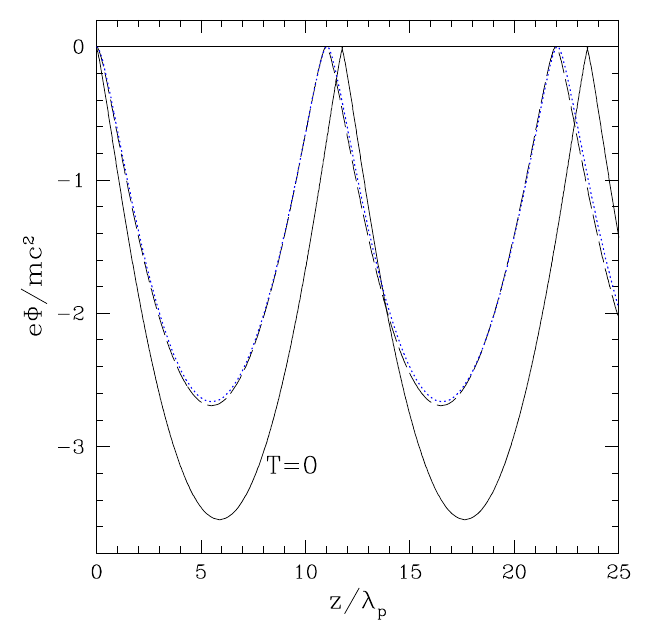
\includegraphics[width=0.7\textwidth]{pics/chap2/f1.png}
  \caption[Steady-state solution for $\alpha < 0$]{Steady-state solution for the
    charge-separated polar-cap flow with $\alpha=0.8$. Two cases are shown: cold
    polar cap $T=0$ (solid curve) and warm polar cap $kT/mc^2=0.03$ (dashed
    curve), which corresponds to average injection momentum $0.22mc$. Dotted
    curve shows the solution for a cold flow where all particles are injected
    with the same $p_0=0.22$. }
\label{fig:steady}
\end{center}
\end{figure}
%%%%%%%%%%%%%%%%%%


\subsection{Cold and warm solutions}\label{sec:solutions}

Once the injection distribution $w(\gamma_0)$ is specified,
it is straightforward to numerically integrate equation~\eqref{eq:steady} and find $a(z)$.
In our sample models we chose
$w(\gamma_0)=(kT)^{-1}\exp[-(\gamma_0-1)/kT]$ with $kT/mc^2=0$ (cold) and
0.03 (warm); the average injection momentum $p_0$ in the warm model equals
$0.22mc$. Figure~\ref{fig:steady} shows $\Phi(z)$ for the cold and warm solutions.

Figure~\ref{fig:steady} also shows a third model where all particles injected at the polar cap
have $p_0=0.22$, i.e. $w(\gamma_0)$ is a delta-function.
In this model, equation~(\ref{eq:steady}) simplifies to
\begin{equation}
\label{eq:cold}
    \frac{\lambda_p^2}{2}\left(\frac{da}{dz}\right)^2 = p(\gamma_0,z)-p_0
                                                                               + \frac{a(z)}{\alpha},
\end{equation}
[same as equation~(3) in B08]. This flow is cold everywhere, i.e. its momentum
distribution is described by $f(p^\prime)=n\,\delta[p^\prime-p(z)]$.
As one can see in Figure~\ref{fig:steady}, the cold model with $p_0\neq 0$ provides an
excellent approximation to the exact warm model that has the same {\it average}
value of $p_0$.

The cold flow solution was discussed in earlier works
% \citep[B08]{1985MNRAS.217..443M}
\citep[B08]{mestel_axisymmetric_1985}
% (Mestel et al. 1985; B08).
For $1-\alpha\ll 1$, the oscillation period is approximately given by (B08)
\begin{equation}
    z_0 \approx 2^{3/2}\frac{\lambda_p}{1-\alpha}, \qquad 1-\alpha\ll 1.
\end{equation}
The precise period is obtained by numerical integration; e.g.
$z_0=11.0\,\lambda_p$ for $\alpha=0.8$.
The momentum of the steady cold flow $p(z)$ oscillates between the injection
momentum $p_0\ll 1$ and a maximum value $p_{\max}$. The minima and
maxima are where $da/dz=0$, and from equation~(\ref{eq:cold}) one finds
\begin{equation}
\label{eq:pmax}
    p_{\max}=\frac{2\alpha\,\gamma_0-(1+\alpha^2)p_0}{1-\alpha^2}.
\end{equation}


\subsection{Stability of the flow}


Although the cold solution with $p_0=0.22$ reproduces very well the electric
potential $\Phi(z)$ of the exact warm solution with the same average $p_0$,
the warm and cold flows are qualitatively different. Their different
momentum distribution functions $f(p,z)$ imply a qualitatively different response
to small perturbations.

Consider first the cold-flow solution
shown by the blue dotted curve in Figure~\ref{fig:steady}.
Since all particles are injected with the same momentum $p_0=0.22$,
all of them follow a single trajectory in the phase space $(z,p)$.
They periodically reach the minimum momentum equal to $p_0$ at
$z_k=kz_0$ ($k=0,1,...$) where potential $\Phi$ reaches maximum.
There are no particles with momenta $p\approx 0$, so
a small perturbation cannot force any particles to reverse their direction of motion,
and hence the perturbation will be advected along the flow.
This flow may be expected to be stable.

In contrast, the warm flow (dashed curve in Figure~\ref{fig:steady}) has a broad
distribution of $p_0$ that extends from $p_0=0$. At each peak of the electric
potential $z_k$ there is a population of particles with nearly zero velocities.
Consider a perturbation at $z\approx z_k$. For example, suppose a small bunch
$\A$ of particles with momenta in a range $(p_1,p_1+\Delta p)$ are slightly
pushed forward while the rest of particles are unperturbed. This perturbation
implies a local increase in electric current $j>j_B$ and hence $\partial
E_\parallel/\partial t<0$ (equation~\ref{eq:Maxw}), generating negative electric
field $\delta E_\parallel$ at $z\approx z_k$ that tends to restore the condition
$j=j_B$. In contrast to the initial perturbation, the induced $\delta
E_\parallel$ affects {\it all} local particles, regardless of their momentum,
not just bunch $\A$. This has two implications: (1) The induced $E_\parallel<0$
will easily and quickly reduce $j$ back to $j_B$ but will be unable to
decelerate bunch $\A$ to the momentum it would have in the steady state flow ---
bunch $\A$ will continue to move to $z>z_k$ with a larger momentum. (2) $\delta
E_\parallel<0$ will give very slow particles $p\approx 0$ negative velocities,
creating a new bunch $\B$ that slides backward down the potential hill. Bunch
$\B$ creates $j<j_B$ at $z<z_k$, and the system reacts there by inducing a small
$\delta E_\parallel > 0$, which accelerates all local particles, regardless
their momenta, not just bunch $\B$. As a result, $j$ quickly recovers to $j_B$,
however, bunch $\B$ is not stopped from moving backward and away from $z=z_k$.

Thus one can see that the perturbation creates permanent damage to the steady
state that broadens the momentum distribution by creating backflowing particles.
This perturbation is {\it not} advected away along the flow, and can develop
further. The backflowing particles turn out to be trapped between two peaks of
the electrostatic potential. Further development can be studied with kinetic
time-dependent simulations; it eventually completely destroys the steady state
solution.


%#################################################################

\section{Numerical setup}
\label{sec:pc-setup}


Our numerical method is similar to that used by
% \citet[hereafter BT07]{2007ApJ...657..967B}
% Beloborodov \& Thompson (2007, hereafter BT07).
\citet[hereafter BT07]{beloborodov_corona_2007}
The plasma is modeled as a large number $N\sim 10^6$ of individual
particles that flow along the magnetic field lines.
We assume that the magnetic field is fixed in
the co-rotating frame of the star; thus $j_B$ and $\rho_\mathrm{GJ}$ are fixed. Then the
problem becomes essentially one-dimensional, as discussed in detail in BT07.
In the present chapter, we consider only charge-separated flows, with no pair creation.
Three other differences from the magnetar simulation in BT07 are as follows:
(1) The magnetar problem had $\alpha\gg 1$
($\rho_\mathrm{GJ}$ was negligible compared with $j_B/c$);
in contrast, $\rho_\mathrm{GJ}$ is crucial for polar-cap flows considered here.
(2) The presence of gravity was essential for the closed-field circuit considered
in BT07, where the global plasma flow was simulated (on a scale comparable to
the radius of the star); in the problem considered here the electric fields are
screened on a much smaller scale $\sim \lambda_p$ and the gravitational
acceleration plays no role.
(3) The flow behavior on the small scales $z\ll \RNS$ may be studied using
a smal computational box $H\ll \RNS$ with an open outer boundary (see below).

In the absence of pair creation, the flow is composed of particles lifted from
the surface; we assume that all of them have the same mass $m$ and charge $e$.
 The particle motion is described by the equation,
\begin{equation}
\label{eq:p}
    \frac{dp_i}{dt} = \frac{eE_\parallel(z_i)}{mc},   \qquad i=1,..,N,
\end{equation}
where $p_i$ is the momentum of the i-th particle in units of $mc$, and
$E_\parallel(z_i)$ is the self-consistent electric field at the particle location $z_i$.
The field is found by integrating Gauss law (equation~\ref{eq:Gauss})
along the magnetic field line,
\begin{equation}
 \label{eq:E}
   E_\parallel(z_i) = 4\pi \left[ eN(z_i) - \rho_\mathrm{GJ} z_i \right].
\end{equation}
Here $N(z_i)$ is the column density of particles between $z=0$ and $z=z_i$,
and we used the boundary condition $E_\parallel(0)=0$, as the material below the
stellar surface is assumed to be a very good conductor that can emit free charges.
Divergence of the perpendicular component of electric field $E_\perp$
is neglected in equation~(\ref{eq:E}) (see BT07 for discussion of this approximation).
The approximation $|\nabla_\perp\cdot\bE_\perp|\ll |dE_\parallel/dz|$ is valid if the
characteristic scale of the flow acceleration $z_0$ is smaller than the transverse
scale $l_\perp$, which is limited by the polar-cap size $\rpc$;
the condition $z_0\ll \rpc$ is satisfied in the dead-zone models presented below.
We also assume that $\rho_\mathrm{GJ}$ is approximately constant on scale $z_0$.
equations~(\ref{eq:p}) and (\ref{eq:E}) in essence describe a relativistic, time-dependent
diode problem with an additional fixed background charge density $-\rho_\mathrm{GJ}$.

As we track the motion of all particles individually, the continuity equation is
automatically satisfied; for a charge-separated flow it is equivalent to charge
conservation,
\begin{equation}
\label{eq:charge}
    \frac{\partial\rho}{\partial t}+\frac{\partial j}{\partial z}=0.
\end{equation}
equation~(\ref{eq:Maxw}) follows from equations~(\ref{eq:Gauss}) and (\ref{eq:charge}),
so we will not need equation~(\ref{eq:Maxw}).
Instead, the parameter $j_B$ enters the problem as a boundary condition.
The magnetic field lines are frozen in the excellent conductor below the stellar
surface, which sustains $j(0)=j_B$.
This condition is enforced in the simulation by injecting the charges in
the computational box at $z=0$ with the fixed rate $j_B$ (BT07).

The electric current $j_B$ is enforced at one boundary $z=0$. Since
the computational box has a finite size $H$, we also have to choose the
boundary condition at $z=H$ and the value of $H$. In all sample models
shown in this chapter we use the simplest boundary condition:
particles moving out of the box are lost and no particles enter the box at
$z=H$. This condition may be refined by allowing a small inflow of returning
particles at the outer boundary. We ran test simulations that show that the
refinements are not important as long as the boundary is sufficiently far,
so that $H$ is much greater than the characteristic scale of the flow acceleration.

In the one-dimensional model, the transverse
gradients are neglected, and the flow effectively has a slab geometry.
Then it is sufficient to follow particles flowing through a small area $A$ of the slab.
This allows one to chose a reasonable number of particles in the computational
box, $N\sim AHn$, e.g. $N\sim 10^6$, so that their dynamics can be followed
in a reasonable computer time. On the other hand,
$N$ should be large enough so that the plasma scale $\lambda_p$ contains
many particles $N_p=A\lambda_p n$.

In summary, we choose $N$ and $H$ so that
\begin{equation}
    \frac{H}{\lambda_p}\gg 1, \qquad N_p=\frac{\lambda_p}{H}\,N \gg 1.
\end{equation}
In this limit, the results are expected to be independent of the choice of $N$ and
$H$ (we verify this by varying the two parameters in Section~3.4). For most of our
simulations $H=100\lambda_p$ and $N\sim 10^6$. Another requirement is a small
time step of the simulation, $\Delta t\ll\omega_p^{-1}$, so that plasma oscillations
are well resolved.


%################################################################

\section{Results}
\label{sec:pc-results}

\subsection{Steady state tests}


In our simulations and in reality the plasma above pulsar polar caps is collisionless.
In the absence of pair creation it must satisfy
%  the collisionless Boltzmann
the Vlasov equation,
\begin{equation}
\label{eq:Vlasov}
    \frac{\partial F}{\partial t} + \mathbf{v}\cdot \nabla F + \frac{d\mathbf{p}}{dt}\cdot \nabla_\mathbf{p} F = 0,
\end{equation}
where $F(t,z,p)$ is the particle distribution function in phase space. The
electric current is $j(t,z)=\rho \bar{v}$ where $\bar{v}(t,z)$  is the average
velocity of the particles. As a first simple test, consider a uniform flow
with $\rho(z)=\rho_\mathrm{GJ}$, $\bar{v}(z)=\alpha c$, and $E_\parallel(z)=0$.
It is easy to see from equations~(\ref{eq:p}), (\ref{eq:E}) and (\ref{eq:Vlasov}) that
the flow must remain in this state. This behavior is reproduced by our simulations.
The steady uniform flow can have any momentum distribution $F(p)$
as long as $\bar{v}=\alpha c$. Note that it requires a continual injection of particles
at $z=0$ with the average velocity $\bar{v}=\alpha c$ (which also requires $0<\alpha<1$).

As a second test, consider a ``cold'' flow where all particles move with
momentum $p(z)$, with zero momentum dispersion. Suppose the flow is injected
at $z=0$ with velocity $v_0<\alpha c$. Then $E_\parallel$ must be generated,
accelerating the flow. In a steady state, the solution for the cold flow must have
the form, $F(z,p^\prime)=n(z)\,\delta[p^\prime-p(z)]$, where $p(z)$ and $n(z)$ can
be described analytically. We first test the special case $\alpha=1$
% \citep{1977ApJ...217..227F}.
% (Michel 1974).
\citep{michel_rotating_1974}.
The flow is accelerated by the self-consistent $E_\parallel(z)$, and $p$ exceeds
unity at $z\sim\lambda_p$. At heights $z\gg \lambda_p$, velocity approaches $c$,
charge density of the flow $\rho=j_B/v$ approaches $\rho_\mathrm{GJ}$, and
electric field $E_\parallel$ asymptotes to a constant value,
\begin{equation}
   E_\parallel=\left[\frac{8\pi m cj_B}{e}\left(\gamma_0-p_0\right)\right]^{1/2}
                      \left[1+{\cal O}(p^{-1})\right],
\end{equation}
where $\gamma_0=(1-v_0^2/c^2)^{-1/2}$ and $p_0=\gamma_0\beta_0$.
Then the flow momentum keeps growing linearly with $z$,
\begin{equation}
     p(z)=\left[2(\gamma_0-p_0)\right]^{1/2}\,\frac{z}{\lambda_p}, \qquad z\gg\lambda_p.
\end{equation}
This solution is reproduced by our simulations with ``cold injection'' --- all injected
particles at $z=0$ have velocity $v_0$. After an initial relaxation period
(comparable to the light crossing time of the computational box) the system
forgot initial conditions and relaxed to the steady state shown in Figure~\ref{fig:alpha1}
(in this example, $v_0=1/6$).
% (\citet{1977ApJ...217..227F}).
The charge density of the flow is large near the polar cap surface and asymptotes
to $\rho_\mathrm{GJ}$ at $z\gg\lambda_p$, as expected.

\bigskip

%%%%%%%%%%%%%%%%%%
\begin{figure}%[h]
% \epsscale{1}
%\epsscale{0.1}
\begin{center}
% \plottwo{f2a.eps}{f2b.eps}
   % \plotone{f2a.eps}\\
   % \plotone{f2b.eps}
  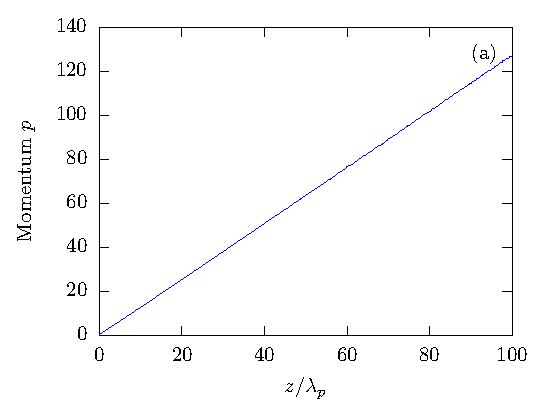
\includegraphics[width=0.6\textwidth]{pics/chap2/f2a.eps} \\
  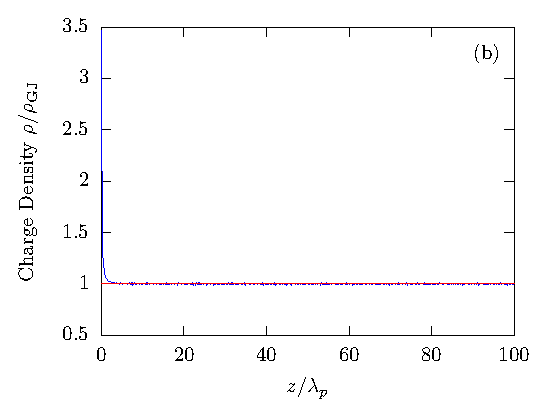
\includegraphics[width=0.6\textwidth]{pics/chap2/f2b.eps}
  \caption[Test run for a cold flow with $\alpha = 1$]{Test run for a cold-flow
    model with $\alpha=1$ and $v_0=c/6$. The flow relaxed to a steady state in
    the entire box $H=10^2\lambda_p$ on the light-crossing timescale, $H/c$; the
    state of the system is shown at $t = 10H/c$. (a) Flow momentum per particle
    $p(z)$ in units of $mc$. (b) Charge density $\rho(z)$.}
\label{fig:alpha1}
\end{center}
\end{figure}
%%%%%%%%%%%%%%%%%%

%%%%%%%%%%%%%%%%%%%
\begin{figure}%[h]
\begin{center}
%\epsscale{0.1}
% \epsscale{1.0}
%\plottwo{f2a.eps}{f2b.eps}\\
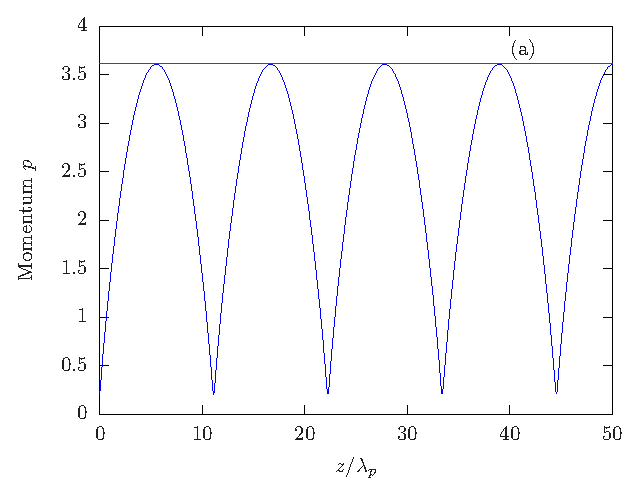
\includegraphics[width=0.6\textwidth]{pics/chap2/f3a.eps}\\
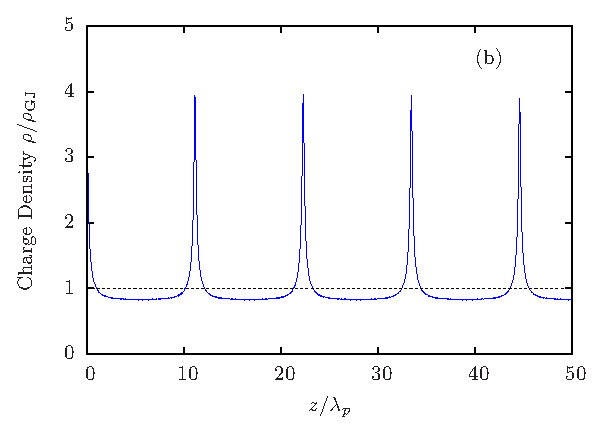
\includegraphics[width=0.6\textwidth]{pics/chap2/f3b.eps}\\
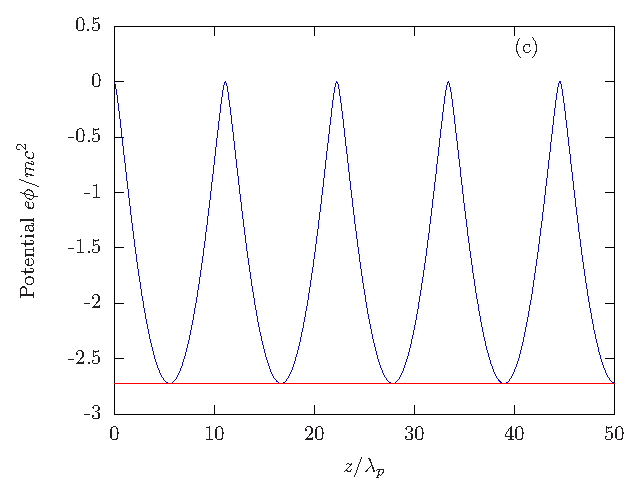
\includegraphics[width=0.6\textwidth]{pics/chap2/f3c.eps}
\caption[Snapshot of a cold flow with $\alpha < 0$]{Cold flow with $\alpha=0.8$ and $\beta_0=0.2$ at time $t=1.45H/c$
%  light-crossing time of the computational box.
% The box is divided into 500 bins and each plotted quantity
% is averaged over the bin.
(a) Momentum $p$ (in units of $mc$). (b) Charge density.
% The charge density peaks are so narrow that they are not fully resolved with
% 500 bins; their true full height is $\rho_{\max}=(\alpha/\beta_0)\rho_\mathrm{GJ}=4\rho_\mathrm{GJ}$.
(c) Electrostatic potential.
}
\label{fig:alpha0.8cold}
\end{center}
\end{figure}
%%%%%%%%%%%%%%%%%%%

Then we studied cold flows with $0<\alpha<1$ and fixed injection velocity $\beta_0$.
We chose in our sample numerical model $\alpha=0.8$ and $\beta_0=0.2$.
The computational box was initially empty; the plasma injected at $z=0$
filled the box on the dynamical timescale
$\sim H/c$ and established a steady state shown in Figure~\ref{fig:alpha0.8cold}.
The steady state is in perfect agreement with the analytical model of \Sect~2.2.
The charge density $\rho(z)$ has spikes at $z=kz_0$ ($k=0,1,...$) where
the flow has the minimum velocity $\beta_0$; the height of each spike is
$\rho_{\max}=j_B/\beta_0=(\alpha/\beta_0)\rho_\mathrm{GJ}$.
The charge spikes are associated with maxima of the electric potential (Figure~\ref{fig:alpha0.8cold}c).
The oscillating momentum has maxima $p_{\max}=3.6$, in excellent agreement
with equation~(\ref{eq:pmax}). The period of oscillation is $z_0\approx 11\lambda_p$, same
as found using the method of \Sect~2.2.

As anticipated in \Sect~2.3, we find that the steady state becomes unstable if we
reduce $\beta_0$ to zero. Then any small perturbation (e.g. due to numerical error)
completely destroys the steady state; instead, a time-dependent state forms, with a
broadened momentum distribution function.
A steady flow with a finite $\beta_0\neq 0$ can also be destroyed, although in this
case a finite,
sufficiently large perturbation is required. In fact, this case provides a better
setup for a numerical analysis of the instability,
as we can control the form of the initial perturbation and then observe how it destroys
the flow that was stable before the perturbation was applied.
We made such an experiment with the flow with $\alpha=0.8$ and $\beta_0=0.2$.
We applied a perturbation that was localized in space and time --- a small ``kick''
$\delta p$ was given to all particles located in a small region $\delta z=\lambda_p/2$;
in this experiment $\delta p$ had a Gaussian distribution with the mean value and
dispersion equal to 0.02.
We observed the following evolution. As the localized
perturbation moved along with the background flow, it was greatly amplified when it
reached the potential maximum (which corresponds to the minimum $p_0\approx 0.2$
of the steady-state solution,
see Figure~\ref{fig:alpha0.8cold}), and some particles acquired a negative momentum, i.e. reversed their
direction of motion. The reversed particles became mostly trapped between two
potential maxima, but some of them were able to penetrate even further back,
beyond the preceding potential peak. The perturbation further spread in the phase space
and the damage to the initial steady-state solution was further amplified with time,
in particular near the potential maxima.
Eventually, the entire flow became strongly time-dependent
and the regular periodic structure of potential peaks disappeared.

The amplification of small (linear) perturbations at the potential maximum can be
understood as follows.
Consider a particle whose Lorentz factor differs from that of the background cold
flow by a small $\delta\gamma$. As the particle moves along with the flow, its deviation
$\delta\gamma$ remains constant, as it travels in the same electrostatic potential as
the background flow (cf. equation~\ref{eq:a}). Using the relation $d\gamma/dp=\beta$, we
find the perturbation of momentum $\delta p$ that corresponds to $\delta\gamma$,
\begin{equation}
    \delta p = \frac{\delta\gamma}{\beta}\propto \beta^{-1}.
\end{equation}
It grows as the particle (and the background flow) decelerates near the potential maximum;
the corresponding amplification factor $\beta_0^{-1}$ is particularly large if
$\beta_0$ is small.

Generation of backflowing particles at the potential peaks $z_k$ plays the key role in
disrupting the steady state. In a flow with a finite minimum velocity
$\beta_0>0$, the external perturbation would need to rob particles
energy $\gamma_0-1\approx \beta_0^2/2$ before they could be reflected by the
potential hill. Thus the gap $\gamma_0-1$ stabilizes the flow against infinitesimal
perturbations, and only a sufficiently strong kick may disrupt the flow.

The trapped or backflowing particles have a deteriorating effect on the steady state
because they are not advected away with the flow and instead repeatedly approach
the same potential peaks, amplifying the perturbations. In addition, one can view
the trapped particles as extra
charge that distorts the electric field. Let $\Ntrap$ be the number of particles
trapped between two potential peaks $z_{k-1}$ and $z_k$; they create electric field
$E^\prime=4\pi e\Ntrap$ at $z>z_k$. The corresponding distortion of the
electrostatic potential $\Phi^\prime=-E^\prime z$ grows linearly with $z$ and
becomes significant at sufficiently large $z$ even if $\Ntrap$ is small.
The distance $z$ required to produce
$e\Phi^\prime \sim mc^2$ is $z\sim (N_p/\Ntrap)\lambda_p$.
This behavior is qualitatively confirmed by our numerical experiments with
larger simulation boxes $H$ --- the flow
was found to become more unstable with increasing $H$.


\subsection{Time-dependent state with warm particle injection}\label{sec:warm}


In a more realistic model, particles are lifted from the polar cap with a thermal
velocity dispersion $\Delta v_0\sim v_0$. The flow still starts with a small velocity
$\bar{v}\ll c$ and hence with a large charge density
$\rho\gg\rho_\mathrm{GJ}$, which self-consistently generates the accelerating electric field.
The basic acceleration mechanism is the same as for the cold flow shown in
Figures~\ref{fig:alpha1} and \ref{fig:alpha0.8cold}. However, there is a new feature:
particles with different
initial velocities behave differently in the collective electric potential, and the charge
density $\rho(z)$ is changed from the cold-flow solution, even though $\Delta v_0\ll c$.
Some particles have $v\approx 0$ and can reverse their motion in the regions of
growing potential ($E_\parallel<0$), which greatly complicates the behavior of the
distribution function $F(z,p)$.

In our simulations, we modeled the warm injection by a one-dimensional Maxwell
distribution, which is a simple Gaussian with dispersion $\Delta v_0$ equal to the
mean value $\bar{v}_0$; we chose $\bar{v}_0=0.2c$.
% Initial conditions are the same as in Section~3.1 (empty computational box).
As initial conditions we took the steady-state solution (\Sect~2).
The main parameter of the flow is $\alpha$, and we calculated the evolution
of the system for several values of $\alpha$ in the range $0<\alpha<1$.
% In all cases, we found that no steady state was established,
As expected, we found that the steady state was quickly destroyed and
the flow kept oscillating in both space and time. The basic parameters of the flow
remained, however, similar to the steady cold model. The average charge density
(averaged over oscillations) is nearly equal to $\rho_\mathrm{GJ}$ and the average velocity $\bar{v}$
is nearly equal to $\alpha c$, so that the condition $\bar{j}=j_B$ is satisfied.
Figure~\ref{fig:meanvelocity} shows the evolution of the hydrodynamic velocity
$\bar{v}(t)$
measured at a fixed location $z_1$ (we chose $z_1=50\lambda_p$, in the middle
of the computational box; $\bar{v}$ was calculated by averaging over
particles inside a small bin around $z_1$, of width $2\lambda_p$).
% After the flow is established in the computational box (in a time $\sim H/c$),
The hydrodynamic velocity $\bar{v}(t)$
% keeps oscillating
oscillates around $\alpha c$;
these oscillations have a relatively small amplitude $\delta v\ll \bar{v}$.

%%%%%%%%%%%%%%%%%%%%
\begin{figure}[h]
\begin{center}
%\epsscale{0.2}
   % \epsscale{1.0}
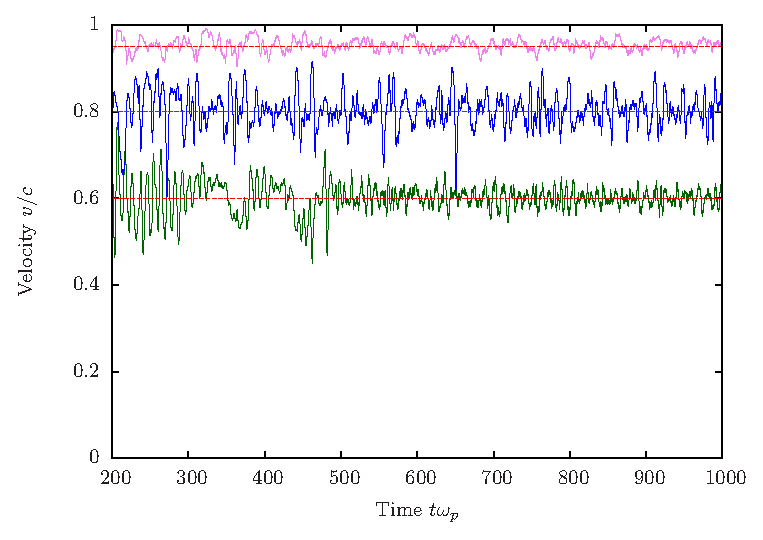
\includegraphics[width=0.8\textwidth]{pics/chap2/f4.eps}\\
%\plotone{f3b.eps}
    %\caption{(a) Evolution of the mean velocity of particles in the box, with $\alpha = 0.83$. The horizontal line plotted in red is $v=0.83$.
    % $x$-axis is in units of the plasma oscillation time $\tau = c/\omega_p$.
    %(b) The evolution of average momentum of particles in time, with $x$-axis in units of plasma oscillation time $\tau = c/\omega_p$.}
\caption[Evolution of $\bar{v}$ over time in the center of the domain]{Evolution
  of the hydrodynamical velocity $\bar{v}$ of the flow measured in the middle of
  the computational box. Three models are shown:
 % in a bin of size $4\lambda_p$ at , with
      $\alpha = 0.95$ (purple), $0.8$ (blue) and $0.6$ (dark green). In all
      three cases, the time-average value of $\bar{v}$ equals $\alpha$. }
    \label{fig:meanvelocity}
    \end{center}
\end{figure}
%%%%%%%%%%%%%%%%%%%%

%%%%%%%%%%%%%%%%%%%%
\begin{figure}% [h]
\begin{center}
% \epsscale{1}
%\epsscale{0.2}
% \plottwo{f5a.eps}{f5b.eps}
  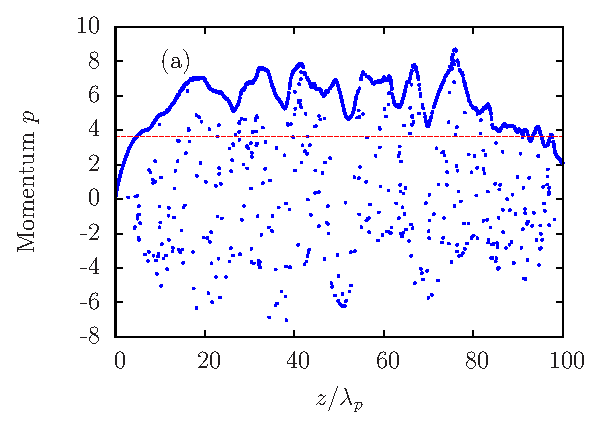
\includegraphics[width=0.6\textwidth]{pics/chap2/f5a.eps}\\
  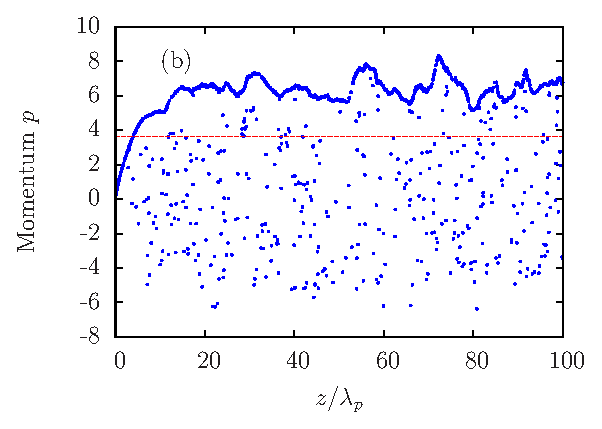
\includegraphics[width=0.6\textwidth]{pics/chap2/f5b.eps}
\caption[Snapshot of particle distribution]{Snapshot of 1000 randomly chosen particles in phase space for the flow
with $\alpha=0.8$ and $\bar{\beta}_0=0.2$.
%Purple curve shows the local mean (hydrodynamical) momentum $\bar{p}(z)$.
% inside a bin of size $\lambda_p/5$, and the r
Red dashed line shows the maximum momentum $p_{\max}$ for the steady cold solution
with the same $\alpha=0.8$ and $\beta_0=0.2$ (Section~3.1).
(a) Random snapshot for the simulation with box size $H = 100\lambda_p$.
(b) Another random snapshot of a similar simulation with a larger computational box
$H = 200\lambda_p$.
% Momentum is in units of $mc$.
}
\label{fig:phasetraj}
\end{center}
\end{figure}
%%%%%%%%%%%%%%%%%%%%


The moderate value of the hydrodynamic velocity does not, in principle, exclude
acceleration of a fraction of particles to much higher energies. We therefore also
studied the momentum distribution of particles in the flow.
Figure~\ref{fig:phasetraj}a shows a random snapshot of the particle distribution in the
phase space for the flow with $\alpha=0.8$.
We randomly chose 1000 particles between $z=0$ and $z=100\lambda_p$
and the figure shows their locations in the two-dimensional phase space $(z,p)$.
The simulation demonstrates the following:

(1) There is no high-energy tail in the momentum distribution.

(2) At each $z$, the momentum distribution has a pronounced narrow peak at
$p_{\rm peak}$. Thus, a large fraction of particles form a cold flow.
The momentum of cold particles
$p_{\rm peak}$ is slightly above the average (hydrodynamical) $\bar{p}(z)$, and
both are above (but comparable to) the value of $p_{\max}$ predicted by the
steady-state model.

(3) There is a low-energy wing in the momentum distribution which extends to
negative momenta (up to 10\% of all particles have $p<0$ in our sample model).
This broad component of the particle distribution has a
hydrodynamic velocity close to zero and does not contribute much to the
current density; however it makes a significant contribution to charge density.
In our sample model, about 20\% of particles reside in the broad component,
and this fact has a simple explanation. From the point of view of the cold stream
dynamics, the broad component provides a background that offsets the effect
of vacuum charge density $\rho_\mathrm{GJ}$ by the fraction of 20\%. This fraction
equals $1-\alpha$, so that the cold
stream may move with $v\approx c$ and carry $j_B$ without the mismatch in
charge density that would generate strong $E_\parallel$. In essence, the broad
component with backflowing particles allows the plasma to self-organize so that
the cold stream can keep $v\approx c$. This is in contrast to the steady-state
solution in \Sect~2, where all particles form a stream with a positive velocity
$v\neq\alpha$, which result in the periodic deceleration and acceleration of the
stream.

% This tail can be viewed as an effective background, which has a
% hydrodynamic velocity close to zero therefore does not contribute to the current
% density, but only changes the effective $\rho_\textrm{GJ}$. The system self-organizes
% such that the effective $\alpha$ becomes close to 1 after the initial acceleration layer.
% About 5-10\% of particles flow backward $(p<0)$.
%In our sample model, about 10 to 15\% of particles reside in the low-energy
%tail. This fraction is determined by the
%fact that the average velocity of the flow must equal $\alpha$ to conduct the required
%electric current. In our sample model $\alpha=0.8$ and hence less than 20\% of particles
%are allowed to have a small (or negative) velocity.
%About 5-6\% of particles flow backward ($p<0$).
%Note that the backflowing particles do not reach the surface $z=0$.
%This is prevented by the potential barrier of the accelerating layer with $\rho\gg\rho_\mathrm{GJ}$
%near the surface. All particles with $p<0$ are eventually accelerated to $p>0$ and
%escape the box through the outer boundary $z=H$.

(4) Both the fluid momentum $\bar{p}(z)$ and the peak momentum $p_{\rm peak}$
fluctuate in time (the corresponding curves in Figure~\ref{fig:phasetraj} move in time).
However, the qualitative form of the
phase-space distribution remains similar to that in Figure~\ref{fig:phasetraj}.

Note that the average momentum $\bar{p}$ does not correspond to
the average velocity $\bar{v}$ shown in Figure~\ref{fig:meanvelocity}, in the sense that
$\bar{p} \neq \bar{\beta}(1-\bar{\beta}^2)^{-1/2}$, because of the broad low-energy tail of
the distribution function. Compared with velocity average,
 the averaging of momentum gives a higher weight to particles with
 large $\beta$ because of the addition factor $\gamma$ in $p=\gamma\beta$.
The average velocity remains close to $\alpha c$, and the averaged momentum is
larger than $\bar{\beta}(1-\bar{\beta}^2)^{-1/2}$.

It should also be noted that the pronounced narrow stream and the broad low-energy stream together
form a two-stream system. Conventionally one would expect the configuration to suffer
from standard micro-instabilities. However, we do not observe such instabilities here.
One important reason is that the
flow remains turbulent even after establishing this quasi-steady state. The momentum
of particles in the colder stream oscillates both in time and space, thus any particle
would not be able to interact with a single wave for an extended period of time. In this
case, exponential growth of particular waves cannot occur, which kills the instability.

As seen in Figure~\ref{fig:phasetraj}a, the flow momentum $p_{\rm peak}$ decreases
near the outer boundary of the computational box $z=H$.
This is an artifact of the boundary condition (free escape with no backflow), which
suppresses backflow density near the boundary. As a result, a modest negative electric
field is induced near the boundary, decreasing $p_{\rm peak}$ so that the flow carries
the required electric current $j_B$.
For comparison, Figure~\ref{fig:phasetraj}b shows a random snapshot of a similar model (in the same interval $0<z<100\lambda_p$) that has twice as large computational box, $H=200\lambda_p$.
As we increase $H$, the boundary effect moves away to larger $z$, affecting the flow
properties only at $z\approx H$. The fraction of backflowing particles measured inside the
box remained unchanged at $\sim$10\%.

%%%%%%%%%%%%%%%%%%%%
\begin{figure}[h]
\begin{center}
%\epsscale{0.25}
   % \epsscale{1.0}
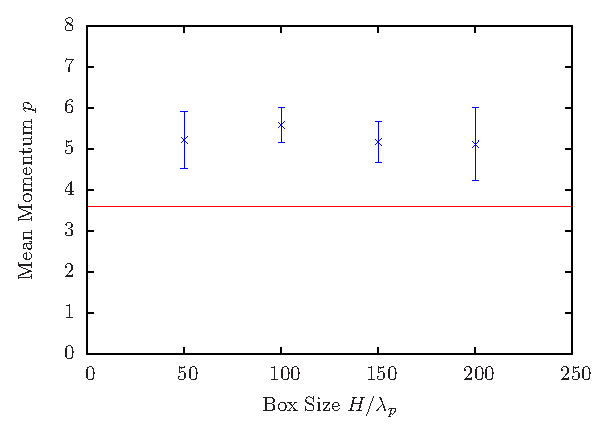
\includegraphics[width=0.7\textwidth]{pics/chap2/f6.eps}
\caption[Mean and standard deviation of particle momentum at the center of the
simulation box]{Mean expectation and standard
  deviation for the fluctuating hydrodynamical momentum of the flow measured at
  the center of the computational box. Four simulations are shown, with box
  sizes $H/\lambda_p=50$, 100, 150, and 200; all four simulations have the same
  parameter $\alpha=0.8$. Red line shows the maximum momentum predicted by the
  steady state model with $\alpha=0.8$.}
% Comparison of the mean momentum in a bin of size $2\lambda_p$ at the center of the box over one light-crossing time of $H_1=100\lambda_p$, plotted for different numerical parameter $H/\lambda_p$, with the same $\alpha = 0.8$. Error bar indicates the standard deviation of the mean momentum.}
\label{fig:zetacompare}
\end{center}
\end{figure}
%%%%%%%%%%%%%%%%%%%%

We also checked whether the flow momentum depends on the size of the computational
box. We ran several simulations with the same $\alpha = 0.8$ and different box sizes
$H$. In each simulation, we measured the fluid momentum $\bar{p}$ in the center of
the box (using a bin $\Delta z=2\lambda_p$) at time $t=100\omega_p^{-1}$.
The results are shown in Figure \ref{fig:zetacompare}.
There is no systematic variation in $\bar{p}$ with the box size; the small variations
($\lesssim 10$\%) are consistent with the fluctuations of $\bar{p}$ in time for each model.

The other numerical parameter of the simulations is $N_p$ (\Sect~3). We checked
that  the results do not depend on $N_p$ as long as it is large; variations in $N_p$
around $\sim 10^4$ did not change the measured parameters of the flow.


%#################################################################

\section{Mixed ion flow and two stream instability}
\label{sec:pc-ions}


If $j_B>0$ (which is equivalent to $\rho_\mathrm{GJ}>0$ for $\alpha>0$), the
charge-separated flow pulled out from the polar cap is made of ions.
Different species of ions may end up in such a flow, and they will be
accelerated to different velocities.

The mixed ion flow shares many features with the identical-particle model
studied in the previous sections. Steady state solutions exist for such flows,
which can be obtained using the method described in \Sect~\ref{sec:solutions}.
Ions with different masses and charges move with different hydrodynamical
momenta and co-exist in a common, periodic electrostatic potential.
This steady solution
is prone to kinetic instability similar to that described in Sections~2 and 4.
%
There is, however, an important new feature: the ion streams with
different hydrodynamical momenta are prone to two-stream instability.

% We modified our numerical setup to investigate the later possibility.
To study the behavior of the mixed ion flow we use a simple modification of
our numerical simulation. Consider a mixture of protons and helium nuclei
(alpha-particles).
The particle injection at $z=0$ now consists of two ions species; they have
charges $e_1$ and $e_2=2e_1$, and masses $m_1$ and $m_2=4m_1$.
The two species are injected with equal rates $\dot{N}_1=\dot{N}_2$.
% and with equal velocities $v_0=0.4c$.
Then alpha-particles carry electric current $j_2=e_2\dot{N}_2$ that is
two times larger than the proton current $j_1=e_1\dot{N}_1$. Thus,
$j_2=(2/3)j_B$ and $j_1=(1/3)j_B$ are maintained at the boundary.

To define a charateristic plasma skin depth $\lambda_p$ we use
equation~(\ref{eq:lambda}) where we replace $e,m,j_B$ by $(e_1,m_1,j_1)$
or, equivalently, by $(e_2,m_2,j_2)$ (note that $e_2j_2/m_2=e_1j_1/m_1$).
The characteristic plasma frequency is defined by $\omega_p=c/\lambda_p$.

% proton and helium respectively.
%They are injected with the same number density???????
%Their injection rates are equal???????
%  and uniform momentum (cold injection), and
% $j_B$ is maintained at the boundary.
% The rest of the simulation setup is similar to that described in section \ref{sec:setup}.

% In fact, a steady state solution exists for such a configuration, and can be found
% using similar method as described in section \ref{sec:solutions}. The solution of
% the electric potential can be found by numerical integration. It again has a periodic
% structure, and the two streams flow independently in the background potential.
% However, this solution is prone to the
% same kinetic instability as the identical particle stream. In addition to that, we
% also observed the development of two-stream instability which further mixes the
% particles in momentum space.

%%%%%%%%%%%%%%%%%%%%%%%%%%%%%%
\begin{figure}[h]
%\epsscale{0.25}
  % \epsscale{1.0}
\begin{center}
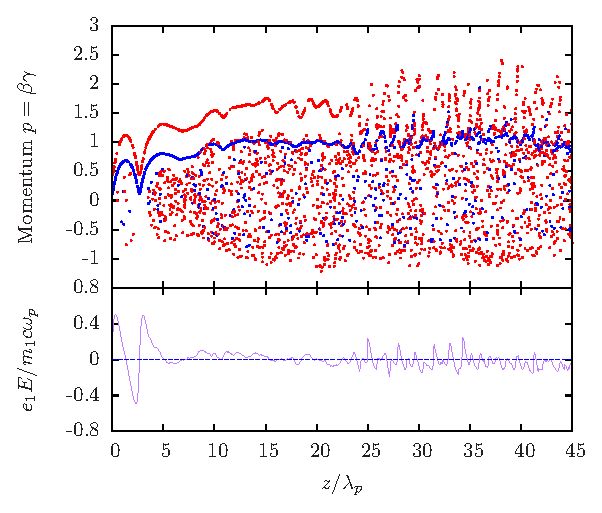
\includegraphics[width=0.8\textwidth]{pics/chap2/f7.eps}
\caption[Snapshot of mixed ion flow]{Snapshot of the mixed ion flow with
  $\alpha=0.4$ at time $t = 10^3\omega^{-1}_p$. Top panel shows the phase space
  distribution, where red dots represent protons and blue dots represent helium
  ions. Bottom panel shows the electric field. }
\label{fig:2stream}
\end{center}
\end{figure}
%%%%%%%%%%%%%%%%%%%%%%%%%%%%%%

Figure~\ref{fig:2stream} shows a snapshot of the phase-space distribution of
ions long after the beginning of the simulation. In this sample model
$\alpha=0.4$; the modest value of $\alpha$ (not close to unity) implies modest
Lorentz factors of particles and fast development of instabilities.
%
% The result of the simulation can be summarized quite well by figure \ref{fig:2stream}.
% The figure illustrates the following features:
The flow exhibits the following features:
% \medskip

\noindent
(1) One period of the steady state solution is reproduced near the injection
boundary $z=0$. The period $z_0\approx 3\lambda_p$ agrees with the result
from numerical integration of the corresponding steady state model.
(This feature is stable in our sample model
because we chose a relatively large injection velocity $v_0=0.4c$.)
% \medskip

\noindent
(2) At larger $z$ the periodic flow becomes unstable and develops into a
configuration similar to that in Figure~5, except that now we have {\it two}
cold variable streams. Besides the cold streams, there is a broad distribution
of ions with smaller momenta and a negligible hydrodynamic velocity.
% which forms an extended wing of the
% distribution function at low momenta.
In our sample model $\alpha=0.4$ and
correspondingly the broad component is self-organized to contain up to
$\sim 60\%$ of particles, so that the streams may move with a relativistic speed
without mismatch in charge density that would generate strong electric fields.
% in both streams of the flow,
% As discussed in \Sect~4, the effect of the broad component on the stream
% dynamics may be viewed as a background that reduces the effective
% $\rho_\mathrm{GJ}$ by a factor of 0.4.
% making the effective $\alpha$ close to unity.
% \medskip

\noindent
(3) Further from the boundary (at $z>20\lambda_p$), the two streams
develop a two-stream instability. The growth rate of the instability may be
estimated using an idealized model of two streams with densities $n_1$,
$n_2$ and velocities $v_1,v_2$. It is straightforward to derive the dispersion
relation for Langmuir modes with frequency $\omega$ and wave-vector $k$
% (e.g. Melrose 1986);
\citep[e.g.][]{melrose_instabilities_1986};
it gives,
\begin{equation}
\label{eq:disp}
    1-\frac{\omega_1^{2}}{\gamma_1^3(\omega - kv_1)^2} - \frac{\omega_2^{2}}{\gamma_2^3(\omega - kv_2)^2} = 0,
\end{equation}
where $\omega_1^2=4\pi n_1 e_1^2/m_1$ and $\omega_2^2=4\pi n_2 e_2^2/m_2$.
Using $\omega_1\approx\omega_2\approx\omega_p$ and the characteristic values
of velocities $v_1,v_2$ from our simulation, we find from equation~(\ref{eq:disp}) that
the most unstable modes have $\omega$ comparable to $\omega_p$ and their
growth rate is $\Gamma\sim 0.1\omega_p$.
% The instability does not happen
% at smaller $z$ because it takes some time to grow. We can estimate the
% growth rate by solving equation (\ref{eqn:twostream}) numerically. For
% modes with reasonable wavelength the growth rate is on the order of
% $\Gamma \sim 0.1\omega_p$.
The distance over which Langmuir waves are amplified is roughly
 $10\lambda_p$.
% to develop siginificant instability, which agrees with our simulation.
As a result of the instabiility, the two streams are smeared out at large $z$,
in particular the stream of lighter ions.
No significant particle acceleration is seen in the simulation.

% The standard dispersion relation for longitudinal Langmuir waves in a two-stream
% configuration is given by (see e.g. Boyd and Sanderson, \emph{The Physics of Plasmas})
% where subscripts 1 and 2 refer to the two ion streams; $\omega_1$ and
% $\omega_2$ are their plasma frequencies. The frequency
% of the fastest growing modes is $\omega\approx 2\gamma_1^{1/2}\omega_1$,
% and the growth rate of the instability is $\Gamma\sim 0.1\omega_p$.


%#############################################################

\section{Discussion}
\label{sec:pc-discussion}

We have presented detailed one-dimensional time-dependent simulations
of the plasma flow extracted from the polar caps of neutron stars.
The simulations provide a fully kinetic description of the flow,
with self-consistent electric field and particle distribution function.
In this chapter, we focused on the regime $0<\alpha<1$, where $\alpha$ is the main
parameter of the flow defined by equation \eqref{eq:alpha}.
In agreement with the estimates of B08, we find that
the particles are accelerated to Lorentz factors,
\begin{equation}
\label{eq:gam2}
   \gamma\approx \frac{1+\alpha^2}{1-\alpha^2},
 \end{equation}
and are not capable of igniting pair creation.
In this sense, flows with $0<\alpha<1$ are ``dead.''
They are sustained by a modest voltage, oscillating in space and time.

The simulations show how a kinetic instability develops and disrupts the ideal
periodic structure found in analytical models of the dead zone (\Sect~2).
We find that the momentum distribution function has two distinct parts --- a
variable ``cold stream'' and a broad wing at low momenta, which includes particles
flowing backward to the polar cap. Even though the flow is turbulent, it shows
no signs of particle acceleration to energies higher than that of the cold stream.

%-----------------------
% Note that the analysis is LOCAL, i.e. the behavior of the flow is controlled
% by the local value of $\alpha=j_B/c\rho_\mathrm{GJ}$, as long as the flow is charge
% separated, and applies to any magnetospheres
% (not necessarily dipole). It also extends to the case where  in a relativistic
% backflow of opposite charge is present; the density of this backflow can be
% included by changing the effective $\rho_\mathrm{GJ}$.
%-----------------------
%MELROSE

The value of parameter $\alpha$ depends
on the location and geometry of the polar cap.
The simplest magnetospheric configuration is that of a centered dipole. Then
the parameter $\alpha$ depends on the angle between the magnetic and spin axes,
$\xi$; besides, it varies across the polar cap. For nearly
aligned rotators ($\xi\approx 0$),
$0<\alpha<1$ in the central part of the polar cap and $\alpha<0$
in a ring-shaped zone near the edge of the polar cap
% (Timokhin 2006; Parfrey et al. 2012).
\citep{timokhin_force-free_2006,parfrey_introducing_2012}
In this case, the dead zone occupies the
central part of the polar cap, and $e^\pm$ discharge must be confined to the ring,
% only the ring is expected to produce $e^\pm$ discharge,
% and radio emission.
matching the phenomenological ``hollow cone'' model of pulsar emission.
% suggested by Goldreich \& Julian (1969).
%  \cite{1969ApL.....3..225R}.
In contrast, the polar cap of an orthogonal rotator ($\xi\approx \pi/2$) has
$|\alpha|\gg 1$, which
% corresponds to efficient particle acceleration and
enables $e^\pm$ discharge
% and radio emission from
for the entire polar cap.
At arbitrary misalignment $0<\xi<\pi/2$,
the values of $\alpha$
% for various $\xi$ is
can be provided by global three-dimensional simulations
of the magnetospheric structure
% (e.g. Spitkovsky 2006)
\citep[e.g.][]{spitkovsky_time-dependent_2006}
and should play a key
role for the geometry of the radio beam.


% On the other hand, in models where $\alpha$ changes across the polar cap, this result provides a description of the ``dead'' regions of the polar cap. Specifically in \cite{1969ApL.....3..225R} it was found that for some pulsar polar caps $\alpha$ changes sign near the boundary, thus creating a ring structure on the polar cap. Inside the ring we have $0<\alpha<1$ which is the ``dead'' region whereas outside the ring we have $\alpha<0$ which will create hugh particle acceleration. If this result can be extrapolated to pulsars which are slightly unaligned, it would predict radio emission patterns with a cone structure, where plasma activity and emissions only take place on magnetic field lines originating near the edge of the polar cap, and the region in the center produces no emission.  Further investigation of this relation would be very interesting.

% This simulation does not include pair creation near the polar cap. Our next goal is to modify the numerical code to include pair creation and investigate the time dependence of the polar cap thickness, for parameters of $\alpha > 1$ or $\alpha < 0$.

We presented our results using plasma skin depth $\lambda_p$ as a unit of
length and particle rest-mass $mc^2$ as a unit of energy. In this form, the results
do not depend on the charge or mass of the particles extracted from the polar cap,
as long as our assumption --- that the flow is made of identical particles --- is
satisfied. In particular, equation~(\ref{eq:gam2}) is valid for both electron flow
($\rho_\mathrm{GJ}<0$) and ion flow ($\rho_\mathrm{GJ}>0$), and the phase-space
distribution shown in Figure~5 describes both cases.
Note that the accelerating voltage is proportional to the particle mass;
voltage implied by equation~(\ref{eq:gam2}) is different for ions and electrons by
the factor of $m_i/m_e\sim 2\times 10^3$.
The relatively high voltage in the ion flow,
$e\Phi\approx\gamma m_ic^2 (1+\alpha^2)/(1-\alpha^2)$,
is still hardly sufficient to ignite $e^\pm$ pair discharge by a seed electron or positron.

The identical-particle model may not hold for an ion flow; in this case,
new effects may enter the problem.
Firstly, heavy ions pulled out from the polar cap may not be completely ionized
and begin to lose electrons as they are accelerated and interact with the X-rays
above the stellar surface; this process effectively creates new charges,
reminiscent of pair creation
% (e.g. Jones 2012).
\citep[e.g.][]{jones_post-glitch_2002}
Secondly, the ion flow may be a
mixture of different nuclei which will be accelerated to different Lorentz factors.
The mixed ion flow is prone to two-stream instability, possibly leading to the formation
of plasma clumps and generation of coherent radio emission.
In our simulations, we observe the expected two-stream instability,
however we do not observe significant structure (clumps) in the turbulent flow.
This may change in three-dimensional simulations.
The frequency of excited waves $\omega\approx 2\gamma_1^{1/2}\omega_1$
is in the radio band, and coherent emission from clumps could create bright
coherent emission. It remains to be seen whether this mechanism
can contribute to the pulsar emission. If it does,
it would create an additional component of the radio pulse.
In the case of aligned rotator, the additional component would be generated in
the central region of the polar cap, leading to a ``hollow cone + core'' structure of
the radio pulse.

% In the case of an ion flow,
% It was proposed that
The charge-separated model of the dead zone can be modified to include possible
backflowing particles from distant parts of the open field-line bundle
(e.g. from a pair-producing outer gap). These particles can contribute to the current
density and also serve as an
additional background charge density, which may be modeled as a contribution to the
effective ``vacuum'' charge density  $-\rho_\mathrm{GJ}$.
This would change the effective $\alpha$
% (Lyubarsky 1992; B08),
\citep[][B08]{lyubarskij_current_1992},
most likely reducing it.
% In particular, if an outer gap produces relativistic $e^\pm$ pairs and sends part of them
% toward the star.

An outer gap is expected to form in a charge-separated flow near the null surface
$\mathbf{B}\cdot\bOm=0$
% (Cheng \& Ruderman 1986)
\citep{cheng_energetic_1986}
. On a given field line, the outer gap will be screened if it is loaded by multiple $e^\pm$ pairs
produced by discharge at the polar cap.
% near the star and loads the field lines with $e^\pm$ flow of a high multiplicity.
Thus, suppression of $e^\pm$ discharge near the field line footpoint is
an essential condition for the existence of an outer-gap accelerator.
% This condition is satisfied only in the dead zone.
Therefore, one can expect an outer gap to form on
field lines with footpoints in the dead zone.

% Outer gap; Parfrey et al. (2012)

We did not simulate in this chapter flows with $\alpha>1$ or $\alpha<0$;
in these cases particles must be strongly accelerated.
This regime leads to an $e^\pm$ discharge that must be unsteady,
with a significant intermittent backflow (B08).
A model for oscillating discharge can be studied in hydrodynamical approximation
\citep{levinson_large-amplitude_2005}
, however a fully kinetic description is essential.
We defer the kinetic time-dependent simulations with pair creation
to a future paper.


% Local Variables:
% TeX-master: "../thesis"
% zotero-collection: #("16" 0 2 (name "Thesis"))
% End:

\zotelo{../thesis.bib}

\def\bB{{\,\mathbf B}}
\def\bE{{\,\mathbf E}}
\def\bS{{\,\mathbf S}}
\def\bJ{{\,\mathbf J}}
\def\bv{{\,\mathbf v}}
\def\Rmax{R_{\rm max}}

\def\rhoGJ{\rho_{\rm GJ}}
\def\IGJ{I_{\rm GJ}}
\def\gthr{\gamma_{\rm thr}}
\def\RLC{R_{\rm LC}}
\def\Rout{R_{\rm out}}
\def\gmax{\gamma_{\max}}
\def\br{{\mathbf r}}
\def\Phipc{\Phi_0}
\def\Phithr{\Phi_\pm}
\def\Phimax{\Phi_\star}
\def\gamLC{\gamma_0}
\def\fLC{f_{\rm LC}}
\def\gdrag{\gamma_{\rm drag}}
\def\bvrot{\bv_{\rm rot}}
\def\bOm{\boldsymbol{\Omega}}
\def\bmu{\boldsymbol{\mu}}
\def\Lsd{L_{\rm sd}}
\def\lav{\bar{l}}
\def\ldisp{\Delta l}
\def\Lin{L_{\rm in}}
\def\Rs{R_{\star}}
\def\rL{r_{\rm L}}
\def\dNi{\dot{N}_i}

\chapter{Global Pulsar Magnetosphere}

\section{Introduction}

The standard picture of pulsar magnetosphere assumes that it is
filled with plasma and  corotates with the neutron star with angular velocity $\Omega$
% (Goldreich \& Julian 1969, hereafter GJ).
\citep[hereafter GJ]{goldreich_pulsar_1969}.  GJ considered the
aligned rotator (magnetic dipole moment $\boldsymbol{\mu}$ parallel to $\boldsymbol{\Omega}$);
then it was generalized to inclined rotators.  The
plasma sustains the ``corotational'' electric field $\mathbf{E}\approx
-\mathbf{v}_{\rm rot}\times \mathbf{B}/c$
(with $\mathbf{v}rot=\boldsymbol{\Omega}\times\br$), which implies the local charge density
$4\pi\rho_\mathrm{GJ}=\nabla\cdot \mathbf{E} \approx -2\boldsymbol{\Omega}\cdot\mathbf{B}/c$.
A key feature of the GJ model is the electric current $I_\mathrm{GJ}$ flowing out of
and into the star along the open magnetic field lines that extend to
the light cylinder $R_\mathrm{LC}=c/\Omega$. GJ showed that the open field
lines are twisted and exert a spindown torque on the rotator.  The
circulating current is $I_\mathrm{GJ}\approx \mu \Omega^2/c$, and the
corresponding spindown power is $\dot{E}\approx \Omega^4\mu^2/c^3$.

This picture was, however, never verified by a first-principle calculation and
was questioned
% (Michel 2004; Gruzinov 2014).
% \citep{michel_state_2004,gruzinov_aristotelian_2013}.
\citep{michel_state_2004, gruzinov_aristotelian_2013}
It was shown that charges lifted from the star by the rotation-induced
electric field form the ``electrosphere''
--- a corotating dome+torus structure,
with a huge gap between them and no electric current
% (Jackson 1976; Krause-Polstorf \& Michel 1985).
\citep{jackson_1976, krause-polstorff_electrosphere_1985}.
Although the electrosphere
is prone to diocotron instability
% (Petri et al. 2001; Spitkovsky \& Arons 2002),
\citep{petri_diocotron_2002,spitkovsky_simulations_2002},
% \citep{petri_diocotron_2002, spi},
it was unclear if it could relax to the GJ state.

In addition to lifted charges, $e^\pm$ pairs are created around pulsars
% (Sturrock 1971).
\citep{sturrock_model_1971}.
This provides plasma capable of
screening the electric field component parallel to the magnetic field, $E_\parallel$.
The negligible plasma inertia and $E_\parallel=0$ provide the ``force-free'' (FF)
conditions, which imply GJ corotation.
The global solution for FF magnetospheres was obtained
using various numerical techniques
% (Contopoulos et al. 1999; Timokhin 2006; Spitkovsky 2006;
% Kalapotharakos \& Contopoulos 2009; Parfrey et al. 2012).
\citep{contopoulos_axisymmetric_1999,timokhin_force-free_2006,spitkovsky_time-dependent_2006,kalapotharakos_three-dimensional_2009,parfrey_introducing_2012}.
Its characteristic feature is a thin current sheet supporting
a discontinuity of $\mathbf{B}$ and the Y-point near the light cylinder.
It was verified with particle-in-cell (PIC) simulations that
sprinkling pairs with a high rate everywhere around the neutron star
would drive the magnetosphere to the FF configuration \citep{philippov_ab_2014}.

A self-consistent model must, however, demonstrate how and where the plasma is
created and to identify the regions of $E_\parallel\neq 0$ (called ``gaps'')
where particles are accelerated to high energies. Besides testing the FF
approximation, the self-consistent model would show how the pulsar
radiation is produced, how the plasma flows in the magnetosphere and gets ejected.
This problem was posed soon after the discovery of pulsars and proved to be difficult.
Three types of gaps were proposed: polar-cap gap
% (Sturrock 1971; Ruderman \& Sutherland 1975)
\citep{sturrock_model_1971,ruderman_theory_1975}, slot gap
% (Arons 1983; Muslimov \& Harding 2004)
\citep{arons_pair_1983,2004ApJ...606.1143M},
and outer gap
% (Cheng \& Ruderman 1986).
\citep{cheng_energetic_1986}.

The only reliable way to solve the problem is a first-principle calculation of the
self-consistent dynamics of the electromagnetic field and pair discharge in the
magnetosphere. Below we present such a direct numerical experiment.
Our simulations are performed with a new 2.5D PIC code, developed from
scratch and designed for neutron-star magnetospheres.
The code calculates the fully relativistic dynamics of particles and fields
on a curvilinear grid, traces the emission of gamma-rays and their conversion to pairs.
The fields obey Maxwell equations, $\partial\mathbf{B}/\partial t=-c\nabla\times\mathbf{E}$ and
$\partial\mathbf{E}/\partial t=c\nabla\times\mathbf{B} - 4\pi\mathbf{J}$, and exert force on particles
$e(\mathbf{E}+\mathbf{v}\times\mathbf{B}/c)$. We use
% Esirkepov (2001)
\citet{esirkepov_2001}
charge-conserving scheme for calculating $\mathbf{J}$
and a semi-implicit algorithm for the field evolution.
A detailed description of the code and tests are given in the accompanying paper
(Chen \& Beloborodov, in preparation).


Pair creation by accelerated particles occurs in two steps: production of gamma-rays
and their conversion to $e^\pm$. In many pulsars, the conversion is only efficient
at $r\ll R_\mathrm{LC}$ where the magnetic field is strong. In young fast pulsars pairs can
be created through photon-photon collisions inside and around
the light cylinder
% (Cheng \& Ruderman 1986).
\citep{cheng_energetic_1986}.
For brevity, we call such rotators
``type I.'' Pulsars with pair creation confined to $r\ll R_\mathrm{LC}$ will be called type II.


%#############################################################
%#############################################################
\section{Problem formulation and simulation setup}


The axisymmetric pulsar is described by its radius $\Rs\approx 10$~km,
angular velocity $\boldsymbol{\Omega}$, and magnetic dipole moment $\boldsymbol{\mu}$ (aligned or
anti-aligned with $\boldsymbol{\Omega}$).  These parameters set the energy scale of
the problem. The neutron star is a nearly ideal conductor, and its
rotation induces voltage $\Phipc\approx \mu\Omega^2/c^2$ across the
footprint of the open field line bundle;
it corresponds to possible particle acceleration up to Lorentz factors
$\gamLC=e\Phipc/m_ec^2$.
We start our simulations with $\Omega=0$ and the vacuum dipole field.
Then we gradually spin up the star: $\Omega$ grows linearly until
it reaches its final value at $t_0=10 \Rs/c$;
$\Omega=const$ afterwards.

Corotational charge density
$\rho_{\rm GJ}\approx -\boldsymbol{\Omega}\cdot \mathbf{B}/2\pi c$
defines the characteristic particle density $n=|\rho_{\rm GJ}|/e$, plasma
frequency $\omega_p=(4\pi ne^2/m_e)^{1/2}$, and skin-depth
$\lambda_p=c/\omega_p$.  The magnetic field also determines the
gyro-frequency of $e^\pm$, $\omega_B=eB/m_ec$, and ions,
$\omega_{B,i}=eB/m_ic$. In a dipole magnetic field
the characteristic frequencies
are related by $\omega_p^2=2\omega_B\Omega$ and satisfy
$\Omega\ll\omega_p\ll\omega_B$.
The particle Larmor radius satisfies
$\rL\ll r$ at $r\ll R_\mathrm{LC}$, so particles move nearly along $\mathbf{B}$. At the light cylinder,
$\rL\sim(\gamma/\gamma_0)R_\mathrm{LC}$ may become comparable to $R_\mathrm{LC}$.

The characteristic $\lambda_p$ at the polar cap is related to particle
acceleration, as $\gamLC\approx (1/4)(\Rs/R_\mathrm{LC})(\Rs/\lambda_p)^2$.
Typical pulsars have $\Rs/\lambda_p\sim 10^6\gg 1$ and $R_\mathrm{LC}/\Rs\sim
10^2-10^3$.  We scale down the big numbers, preserving the hierarchy
of scales. The scale $\lambda_p$ must be well resolved in the
simulation, and the number of particles per grid cell must be large.
This can only be achieved by increasing $\lambda_p/\Rs$.
The simulations presented below have
$\Rs/\lambda_p\approx 100-130$, $R_\mathrm{LC}/\Rs=6-10$, and  $\gamLC=425$.
We also reduced the ion mass, $m_i=5m_e$,
and assumed ion charge number $Z=1$.

We use spherical coordinates $r,\theta,\phi$, and our grid is uniformly spaced
in $\log r$ and $\theta$ to allow better resolution near the star, where it is most
needed. The grid size is $512\times 512$.

Three field components are continuous at the star surface which defines
the boundary conditions: $B_r=2\mu\cos\theta/\Rs^3$, $E_{\theta} =
-\mu\Omega\sin 2\theta/\Rs^2$, and $E_\phi=0$.
The dipole configuration of the magnetosphere is set by the surface $B_r$, and
its rotation is communicated from the star through the surface $E_\theta$.
The star is also a source of electrons and ions for the magnetosphere.
We make both particle species available below the surface and their extraction
is self-consistently controlled by the local electric field.  We neglect the work function,
so that particles are easily lifted from the star.

The outer boundary is set at $\Rout=30\Rs\gg R_\mathrm{LC}$.
Here we place a ``damping layer'' of thickness $\Delta R=\Rout/15$.
The layer has resistivity and damps electromagnetic fields on
a timescale $\sim\Delta R/c$.  Particles escape freely; they
are decoupled from the fields once they enter the damping layer.  With
this implementation, the boundary effectively absorbs waves and
particles, which is equivalent to their free escape.

Once an electron or positron reaches the threshold energy $\gthr
m_ec^2$ it begins to emit curvature photons capable of pair creation.
It depends on the curvature radius of the particle trajectory $R_c$ as
$\gthr= K (R_c/\Rs)^{1/3}$. In real pulsars $K\gtrsim 10^6$; we scale
it down to $K=20$ to allow copious pair creation in our numerical
experiment.
The photon emission rate is $\dot{N}=0.25 c(\gamma/R_c)$,
where $\gamma$ is the particle Lorentz factor.
The photon emission, propagation, and conversion are
traced using Monte-Carlo technique.  The free paths of photons $l$
have a distribution $P(l)$ with mean value
$\lav$ and dispersion $\ldisp$. The extreme case of $\lav=0$ is only relevant for
discharge near magnetars \citep{beloborodov_corona_2007};
for ordinary pulsars, the delay $l/c$ should be included. In our simulations
$\lav=\ldisp=2\Rs$ for photon-photon collisions
(operating in rotators of type~I)
and $\lav=\ldisp=0.2\Rs$ for magnetic conversion (enabled at $r\lesssim 3\Rs$).
The emitted photons have energies $E_{\rm ph}\ll \gthr m_ec^2$, and hence
the secondary pairs are created with Lorentz factors $\gamma_s\ll\gthr$.
The condition $\gamma_s\ll \gthr\ll\gamLC$ ensures sufficient pair supply in the
magnetosphere, and is satisfied in our simulations.
Radiation reaction (energy loss due to gamma-ray emission) is
explicitly included in the particle dynamics.

Hereafter distance is measured in $\Rs$, time in $\Rs/c$, energy in $m_ec^2$,
magnetic and electric fields in $m_ec^2/e\Rs$, and
charge density in $m_e c^2/4\pi e\Rs^2$.


%###############################################################
%%%%%%%%%%%%%%%%%%%%%%%%%%%%%%%%%%%%%
\begin{figure}[t]
 %   \centering
 \hspace*{-0.6cm}
    \includegraphics[width=1.07\textwidth]{pics/chap3/figure1.eps}
    \caption{\small
    Magnetosphere of type I aligned rotator (poloidal cross section) at $t = 100$.
    Vertical dashed line shows the light cylinder.
    Green curves show the magnetic flux surfaces.
    (a) Radial component of electric current density $J_r$.
           (b) Net charge density $\rho$.
           (c) Toroidal component of the magnetic field $B_\phi$.
 }
    \label{fig:j-rho-bphi}
\end{figure}
%%%%%%%%%%%%%%%%%%%%%%%%%%%%%%%%%%%%%

\section{Rotators of type I}


Figures~\ref{fig:j-rho-bphi}--\ref{fig:gamma-U-photon} show the magnetosphere of the
aligned rotator with $R_\mathrm{LC}=6$ and $\mu=1.5\times 10^4$ after 2.6 rotation periods.
The energy density is almost everywhere dominated by the electromagnetic
field, and the discharge finds a way to adjust and supply the charge density and
electric currents demanded by the field. As a result, the magnetosphere
shares several key features with the FF solution.
Electric currents and Poynting flux flow through the light cylinder along
the open magnetic field lines while the interior of the closed field-line zone
has $\mathbf{J}=0$ and $B_\phi=0$. The Y-point is observed near $R_\mathrm{LC}$.

There are two distinct regions of negative and positive radial current density $J_r$.
The negative current flows in the polar region around the magnetic axis.
The positive current is concentrated in a current sheet supporting
the jump of $B_\phi$ between the closed and open zones.
Outside the light cylinder, the current sheet extends along the equatorial plane
to support the flip of $B_\phi$ and $B_r$ across the equatorial plane.

%%%%%%%%%%%%%%%%%%%%%%%%%%%%%%%%%%%%%
\begin{figure}[t]
%    \centering
\hspace*{-0.6cm}
    \includegraphics[width=1.07\textwidth]{pics/chap3/figure2.eps}
    \caption{\small
Charge densities of (a) positrons, (b) electrons, and (c) ions.
}
    \label{fig:rho-pn-corotation}
\end{figure}
%%%%%%%%%%%%%%%%%%%%%%%%%%%%%%%%%%%%%

Charge density $\rho=\nabla\cdot \mathbf{E}/4\pi$
also conforms to the expectations from the FF model
\citep[cf. Figure~16 in][]{parfrey_introducing_2012}.
In particular, the current sheet is positively charged outside the Y-point and
negatively charged inside the Y-point
(see Timokhin 2006 for discussion).
% \citep[see][for discussion]{timokhin_force-free_2006}.
$\rho$ significantly deviates from the FF model in the neutral black region with
$J_r=0$; if the rotator approaches the ``death line''  for pair creation,
$\gthr\sim\gamLC$, this region grows and occupies most of the magnetosphere.
A similar neutral
 region was described by
% Yuki \& Shibata (2012).
 \citet{yuki_particle_2012}.

%%%%%%%%%%%%%%%%%%%%%%%%%%%%%%%%%%%%%
\begin{figure}[t]
    \centering
    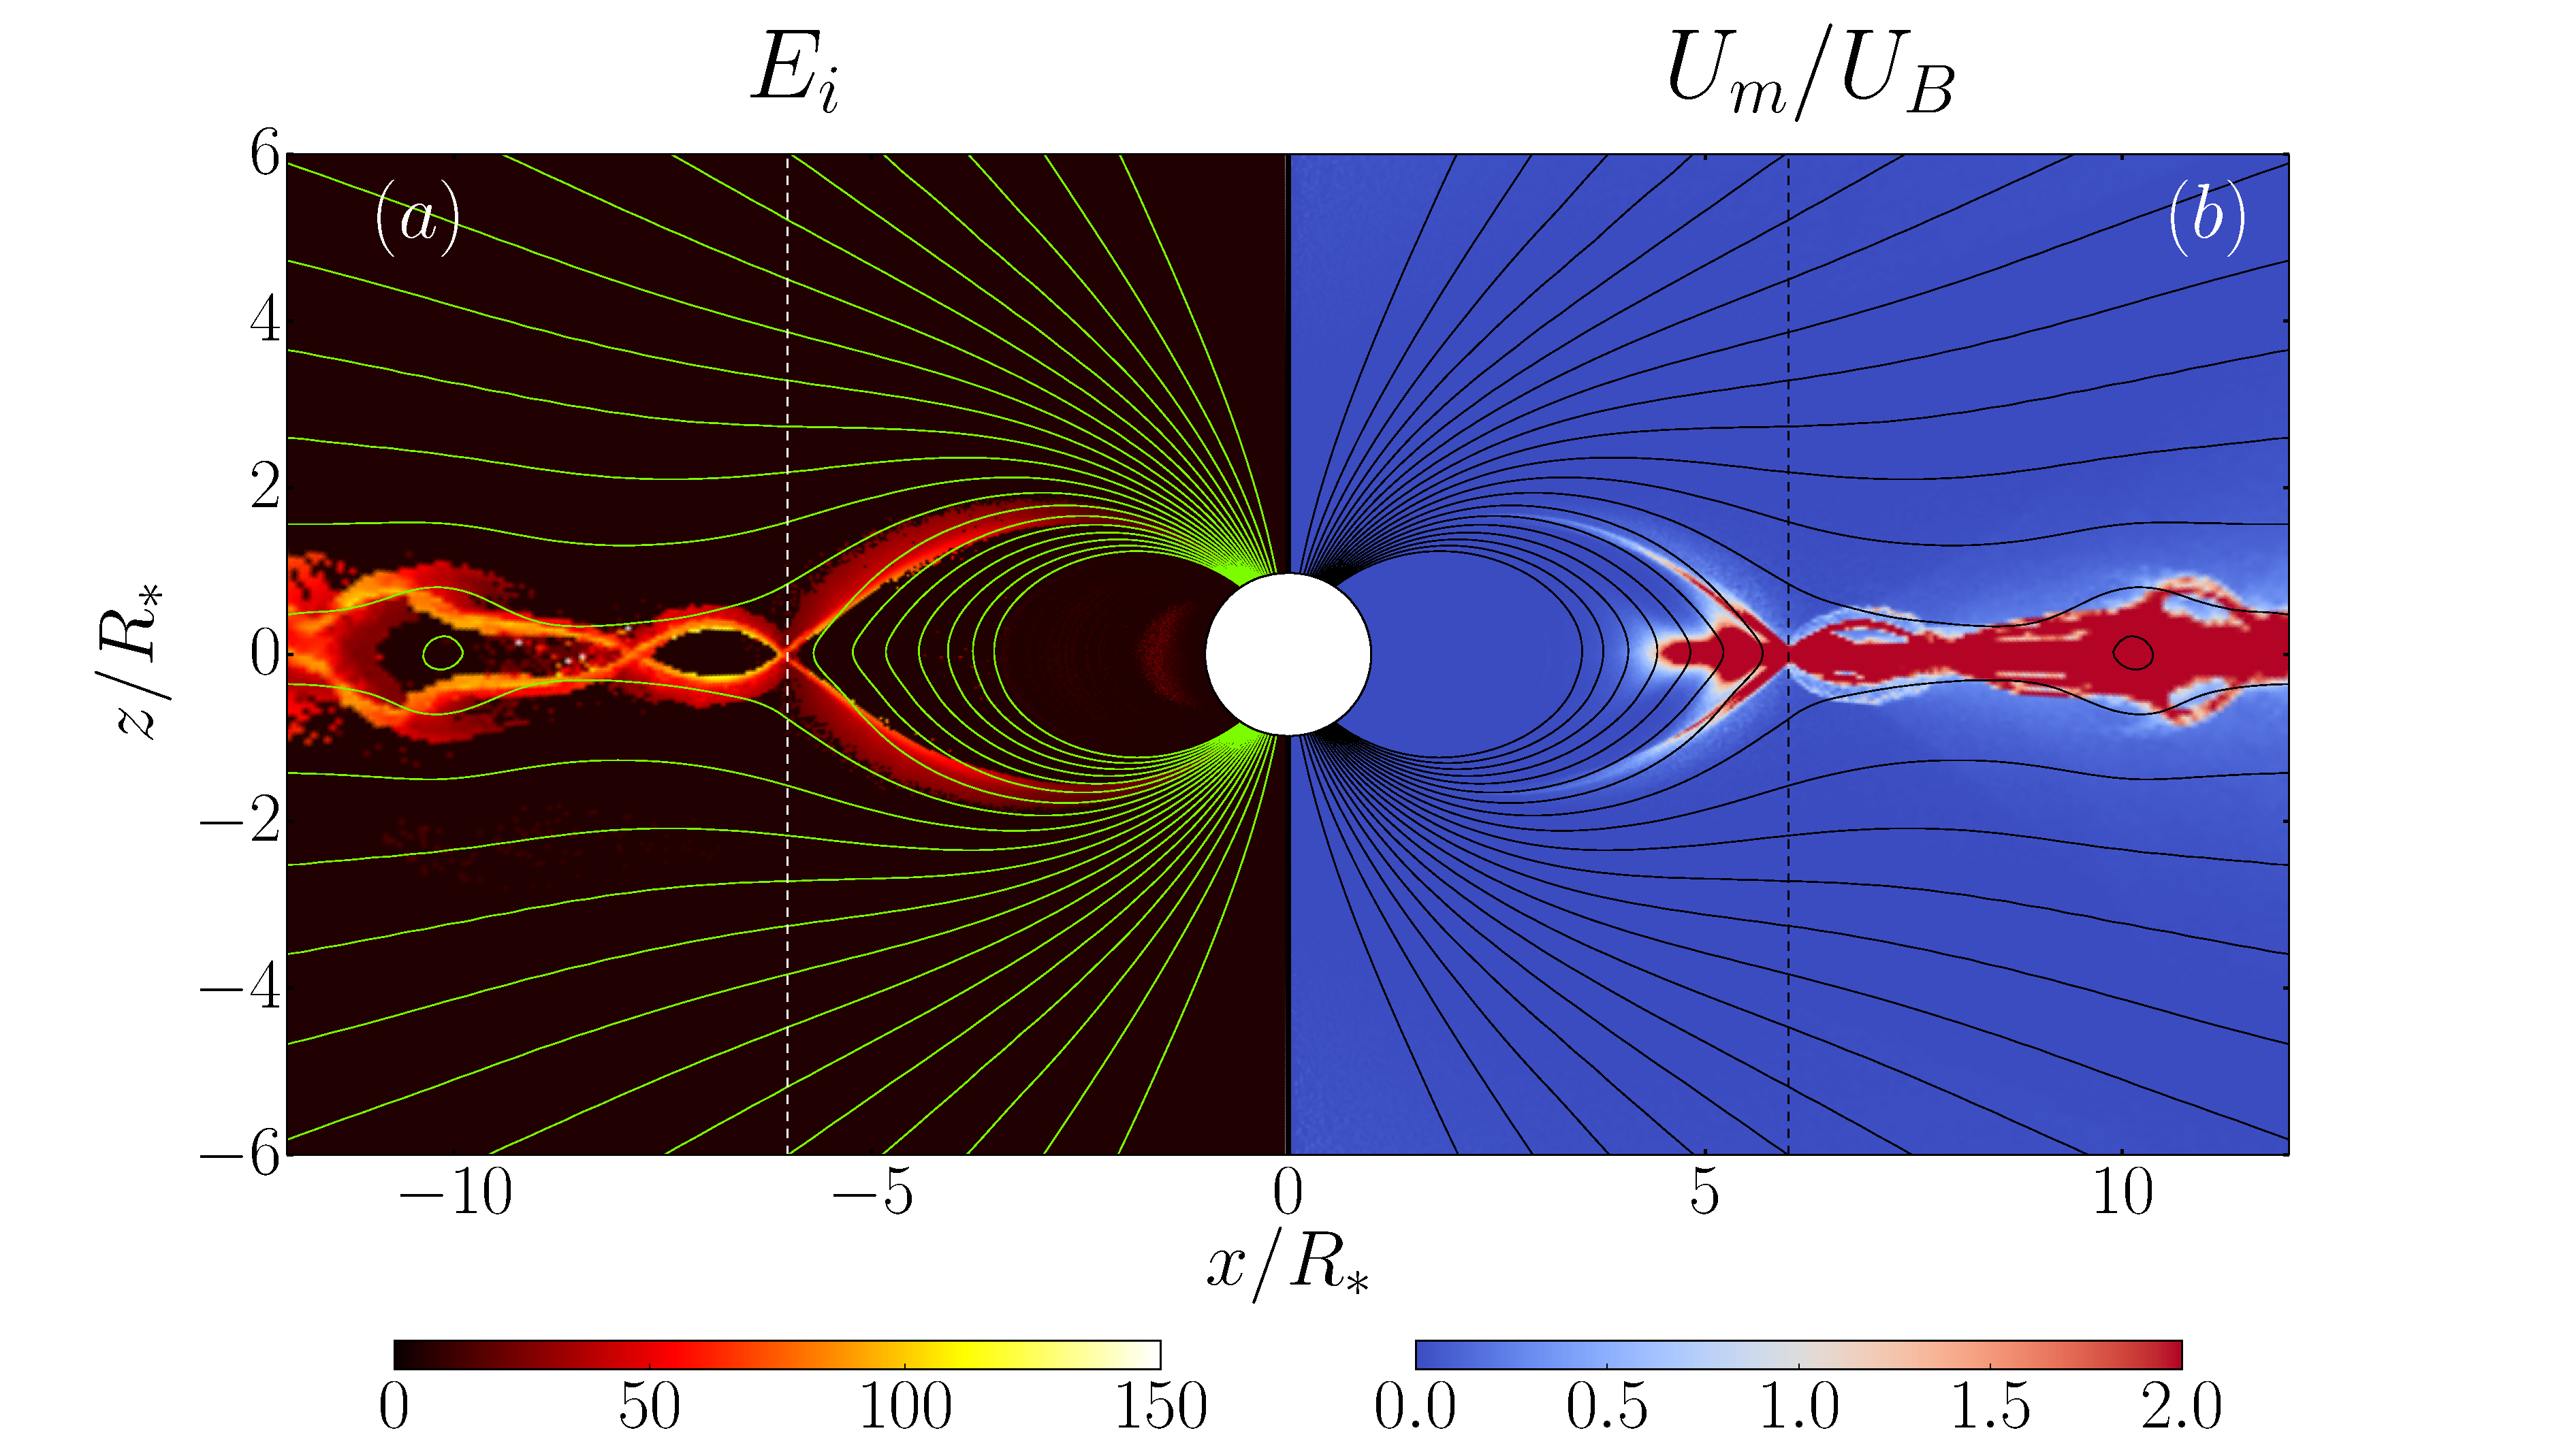
\includegraphics[width=0.85\textwidth]{pics/chap3/figure3.eps}
    \caption{\small
    (a) Average ion energy in units of $m_ec^2$. (b) Ratio of total matter energy density
    $U_m$ to magnetic energy density $U_B=B^2/8\pi$.
}
    \label{fig:gamma-U-photon}
\end{figure}
%%%%%%%%%%%%%%%%%%%%%%%%%%%%%%%%%%%%%


The two opposite currents are sustained by different mechanisms.
The negative current in the polar region is carried by electrons lifted
from the polar cap. There is no significant activity in this region;
the particle acceleration is weak and pair creation does not occur. The absence
of polar-cap activity is explained by the low positive value of
$\alpha\equiv J_\parallel/c\rho_\mathrm{GJ}\sim 0.7 <1$.
It leads to easy screening of $E_\parallel$ by the charge-separated
flow extracted from the star and the flow Lorentz factor
comparable to $2\alpha/(1-\alpha^2)$
% (Beloborodov 2008; Chen \& Beloborodov 2013).
\citep{beloborodov_polar-cap_2008,chen_dead_2013}.
We observed the same behavior in the simulation of anti-aligned rotator where currents
switch sign and the polar current is carried by ions extracted from the star.

The opposite current (the current sheet) is sustained by $e^\pm$ discharge
at $r<R_\mathrm{LC}$.
It cannot be conducted by particles lifted
from the star as its sign is opposite to that of the
charge density demanded by the magnetosphere. Note also that
$|\rho|\gg|\rho_\mathrm{GJ}|$ in the current sheet, so $\rho_\mathrm{GJ}$
is not important. The accelerating potential drop
is $\Phi_\parallel\sim 2\pi \rho\delta^2 \sim -(\delta/r)\Phi_0$ where $\delta$ is the
sheet thickness and we used $2\pi  r\delta |\rho| c\sim I_\mathrm{GJ}=c\Phipc$.
Pair creation is biased to the outer side of the sheet (a result of its curvature
and the finite free path of photons), therefore the unscreened $\Phi_\parallel$ is largest
on the inner side. The sheet thickness $\delta$ is set by the Larmor radius of particles
near the Y-point.

Plasma outflows along the equatorial plane outside $R_\mathrm{LC}$
and the Y-point resembles a nozzle formed by the open magnetic fluxes of opposite
polarity. Two plasma streams come to the Y-point along the boundary of the closed
zone and exchange their opposite $\theta$-momenta.
Their collimation is achieved through gyration in the (predominantly toroidal)
magnetic field, which communicates the $\theta$-momentum from one stream to the other.
As a result the streams flow out in the direction of their net momentum, which is radial
% (see also Shibata 1985).
\citep[see also][]{shibata_self-consistent_1985}.

About $10$\% of current is carried by the ions
extracted from the star at the footpoints of the current sheet.
Ions experience no radiative losses and tap the full $\Phi_\parallel$
(Figure~\ref{fig:gamma-U-photon}a). They have the largest Larmor radius
$\rL$, so the ion streams show large oscillations around the equatorial plane
(Figure~\ref{fig:rho-pn-corotation}c). The streams with smaller oscillations are formed by
accelerated positrons with $\gamma$ limited by radiation reaction.
Secondary particles have
even smaller energies; they outflow almost exactly in the equatorial plane.
The streams with different $\rL$ contribute to the thickening of the equatorial
current sheet as seen in Figures~\ref{fig:j-rho-bphi}-\ref{fig:gamma-U-photon}.


Since ions do not create pairs, the discharge in the current sheet
relies on the accelerated $e^\pm$. This requires continual recycling
of created particles as seeds for new rounds of pair creation, which
leads to voltage oscillations.
The oscillations occur on the timescale $\sim R_\mathrm{LC}/c=\Omega^{-1}$ and make the
magnetosphere ``breath'' around $R_\mathrm{LC}$.

There is a steep potential drop across the outer closed field lines toward the
Y-point. The strong $E_r$ helps eject particles into the equatorial current sheet.
In this region $E\approx B$ and the particle ejection across $\mathbf{B}$ is assisted by
the drop of $B$ near the $Y$-point on a scale $\sim\rL$.

The magnetic field dominates energy density everywhere except the Y-point region
and the matter-dominated equatorial outflow (Figure~\ref{fig:gamma-U-photon}b).
This behavior is also visible in the angular distributions of the Poynting luminosity
$L_P$ and matter kinetic power $L_m$ (Figure~\ref{fig:fluxes}a).
The integrated luminosities at $r=2R_\mathrm{LC}$ are $L_P\approx 0.7 L_0$ and
$L_m\approx 0.15 L_0$ where $L_0=\mu^2\Omega^4/c^3$.
Both contribute to the energy flux from the rotator.
This should be compared with the spindown power extracted from the star,
$\Lsd=L_P(\Rs)\approx 0.88L_0$.
The difference between $\Lsd$ and
$L_P+L_m$ is carried by particles bombarding the star
(the backflow power is $\sim 0.1L_m$) and the gamma-rays.

At $r\gg R_\mathrm{LC}$ we observe magnetic reconnection which strongly heats
particles in the equatorial outflow, forms large plasmoids, kinks and wiggles.
They are advected outward and do not affect the current structure near the Y-point.

The current sheet is the only source of gamma-rays (Figure~\ref{fig:fluxes}b).
The emission is strongly anisotropic, peaking at
$\pm \sim 12^{\circ}$ around the equatorial plane. In addition,
there is a strong peak at the equator from the high-energy
particles gyrating in the equatorial outflow.

%%%%%%%%%%%%%%%%%%%%%%%%%%%%%%%%%%%%
\begin{figure}[t]
   % \centering
    \hspace*{-0.6cm}
    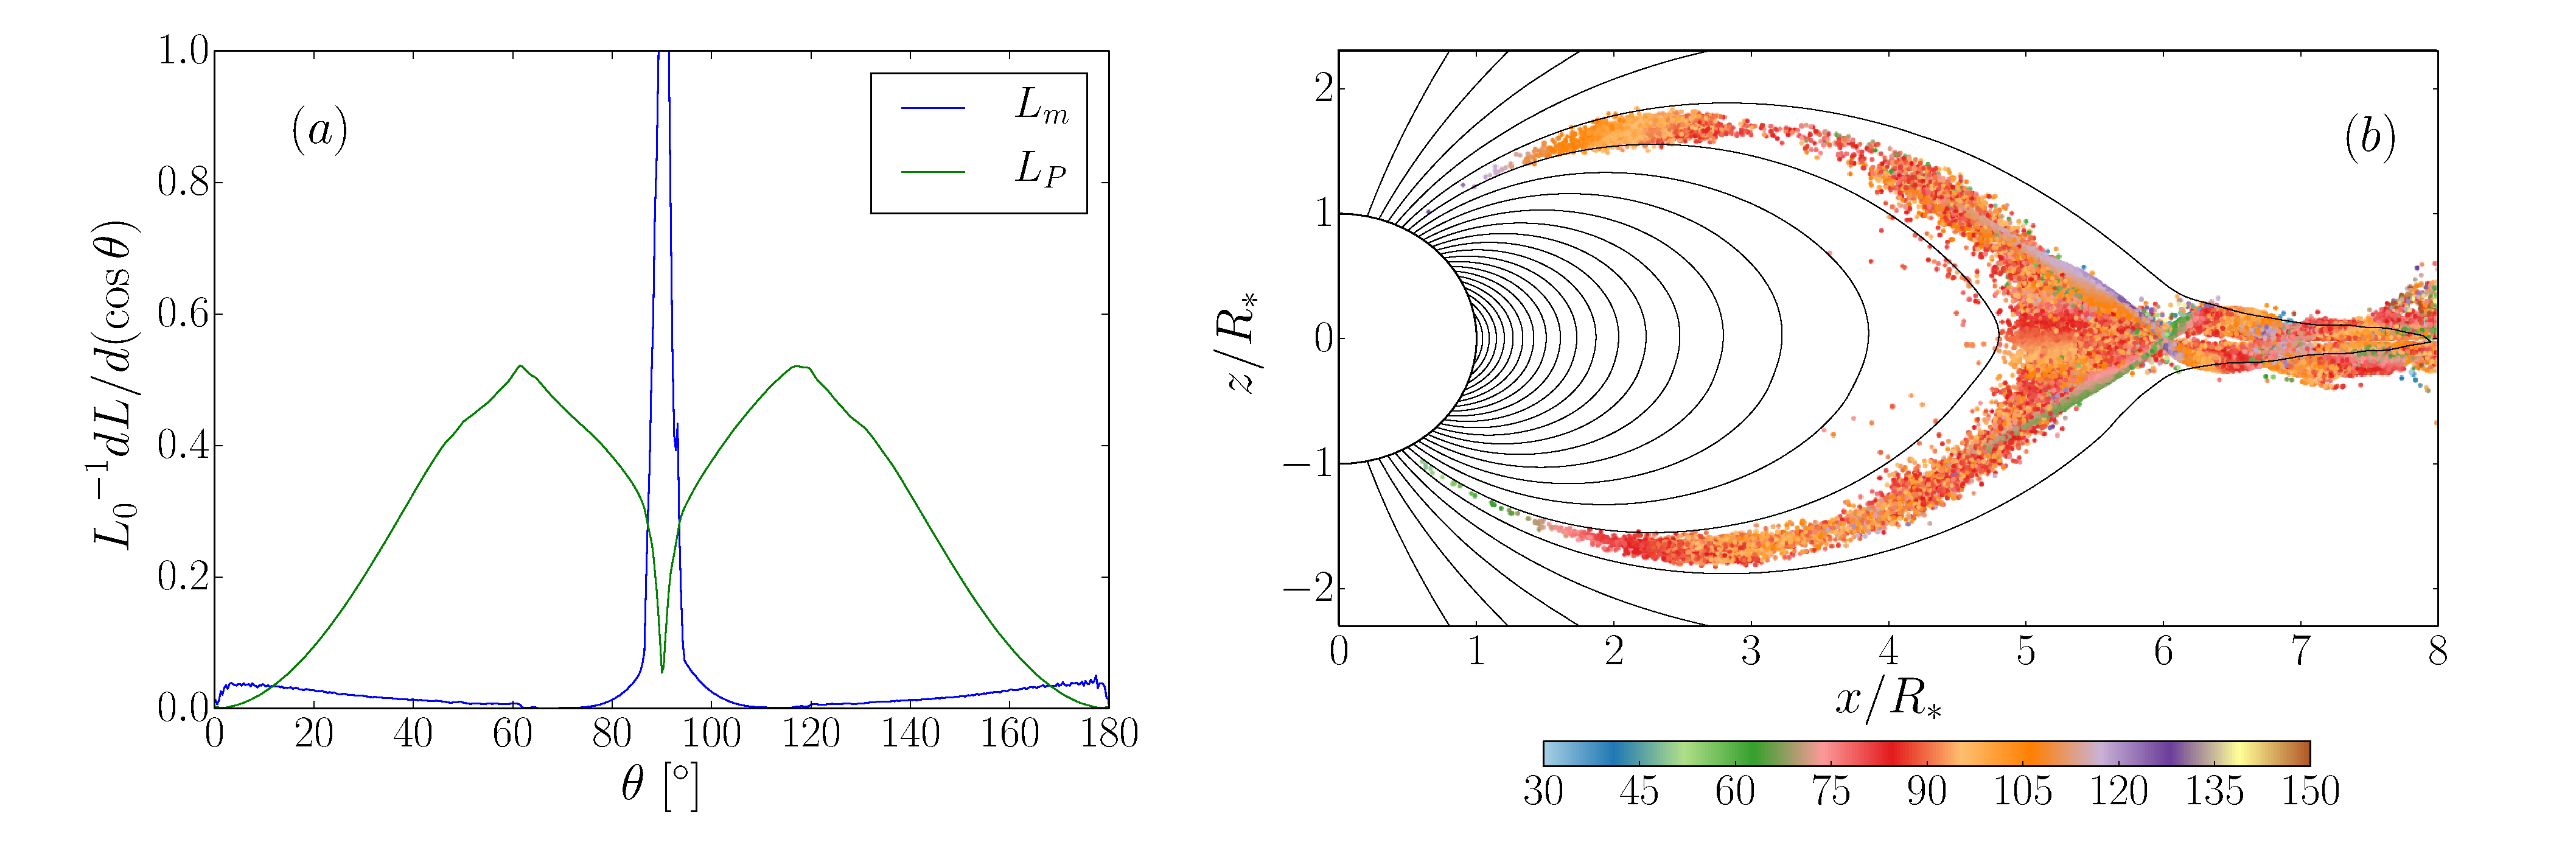
\includegraphics[width=1.07\textwidth]{pics/chap3/figure4.eps}
    \caption{\small
        (a) Angular distribution of
        Poynting flux $L_P$ and kinetic energy flux $L_m$ at radius
        $2R_\mathrm{LC}$, normalized to  $L_0 = \mu^2\Omega^4/c^3$.
        (b) Locations of gamma-ray emission
        events. Color shows the angle of the photon
        direction with respect to $\hat{\mathbf{z}}$.
          }
    \label{fig:fluxes}
\end{figure}
%%%%%%%%%%%%%%%%%%%%%%%%%%%%%%%%%%%%


The simulation for the anti-aligned rotator shows a similar magnetosphere
but somewhat different discharge.
The current sheet extracts
and accelerates electrons from the star
(instead of ions), which helps
produce pairs. This leads to a more stable $\Phi_\parallel$
and reduces the ``breathing'' of the magnetosphere, so the Y-point is nearly static.

We also performed runs for the aligned and anti-aligned rotators with
different rotation rates, magnetic fields, and $\gthr$. The exact
position of the Y-point $R_Y$ depends on these parameters.
With extremely low $\gthr$ and copious supply of plasma $R_Y$ decreases.
If $\gthr/\gamLC$ is increased to $\sim 1$,
the magnetosphere transitions to the electrosphere state.

%###############################################################

\section{Rotators of type II}

The simulation of type~II rotators is the same as for type~I except for three changes:
we suppressed pair creation where $B<400$, which roughly corresponds to $r\gtrsim 4$,
increased $R_\mathrm{LC}$ to 10 to better separate it from the pair creation zone,
and increased $\mu$ to $2.5\times 10^4$ to keep $\Phipc$ unchanged.


As we spin up the star, there is an initial burst of pair creation due to the
vacuum initial condition and the induced $E_\parallel$ accelerating
charges extracted from the surface. The system is able to form an almost FF
configuration for a short time, then $E_\parallel$ gets screened inside the
pair-creation zone, and the magnetosphere relaxes to a different state.
After about 2 rotations of the star, $\rho\approx\rho_\mathrm{GJ}$ is sustained only at $r\lesssim 4$,
and outside this zone the magnetosphere is close to the electrosphere solution
(Figure~\ref{fig:type2}). It stays in this state till the end of the simulation
(about 8 rotations), with no pair creation.

%%%%%%%%%%%%%%%%%%%%%%%%%%%%%%
\begin{figure}[t]
    \centering
    \includegraphics[width=0.85\textwidth]{pics/chap3/figure5.eps}
    \caption{\small
    Type II magnetosphere at $t=280$.
    (a) Parallel electric field $E_{\parallel}$.
    (b) Charge density $\rho$.
    }
   \label{fig:type2}
\end{figure}
%%%%%%%%%%%%%%%%%%%%%%%%%%%%%%

In the final state, the magnetic field is everywhere similar to the dipole.
The plasma forms the negative ``dome'' and positive ``torus''
with a vacuum gap between them at $r\gtrsim 4$.
The gap is outside the pair-creation zone and finds no way for plasma supply.
The unscreened $E_\parallel$ in the gap creates a
large potential drop along the
magnetic field lines, which leads to faster rotation of the magnetosphere in the
equatorial region at $r\sim 5-8$
% \AB{(cf. Wada \& Shibata 2011).}
\citep[cf.][]{wada_particle_2011}.

The magnetosphere is not completely dead at the end of the simulation.
There is a weak negative current flowing out in the polar cap region, and
a weak positive current leaking out from the tip of the ``torus'' region
due to a strong $E_r\approx B$.
At later times we expect the magnetosphere to evolve even closer to
the electrosphere solution.  The gap will tend to expand toward the
null point $\rho_\mathrm{GJ}=0$
on the star surface, into the zone where pair creation is
possible. Then the discharge should reignite and prevent the inward
expansion of the gap. The duration of our simulation is too short to
see this late evolution; however, it is sufficiently long to show that type
II rotators have a low level of activity most of the time.

Breaking the axisymmetry should initiate the diocotron instability
% (e.g. Philippov \& Spitkovksy 2014);
\citep{philippov_ab_2014};  however it is unlikely to
prevent the inner zone from filling with plasma and
shutting down pair creation. Our simulations suggest that type II rotators
cannot relax to the GJ state
--- it is unstable even with suppressed azimuthal perturbations; allowing the
diocotron instability cannot make the GJ state an attractor for the system.


%################################################################

\section{Discussion}


Our first conclusion is that significant activity of the axisymmetric pulsar
requires pair creation enabled at $r\sim R_\mathrm{LC}$
(called type I in this paper); this requires a sufficient optical
depth to photon-photon collisions.
If pair creation is limited to $r\ll R_\mathrm{LC}$ (type II),
the return current is choked and the axisymmetric magnetosphere relaxes to the
dome+torus state with suppressed electric currents and pair creation.
Many observed pulsars are only capable of pair creation at
$r\ll R_\mathrm{LC}$; we conclude that their activity and spindown should
be a result of the misalignment of $\boldsymbol{\Omega}$ and $\boldsymbol{\mu}$. This conclusion
supports the arguments of
% Michel (2004)
\citet{michel_state_2004}
 and disagrees with the models of
% Goldreich \& Julian (1969),
\citet{goldreich_pulsar_1969},
% Ruderman \& Sutherland (1975),
\citet{ruderman_theory_1975},
and
% Gruzinov (2014).
\citet{gruzinov_aristotelian_2013}.

Type I axisymmetric rotators are active, as long as discharge voltage
$\Phi_{\rm thr}<\Phi_0=\mu\Omega^2/c^2$.
Their spindown power is $\Lsd\approx \mu^2\Omega^4/c^3$
and their magnetic configuration is similar to the FF solution.
Our numerical experiment shows, for the first time,
how particle acceleration and $e^\pm$ discharge
self-organize to maintain this configuration.
The result is quite different from the
previously discussed ``trio'' of gaps: polar-cap gap, slot gap, and outer gap.
Neither aligned nor anti-aligned rotators sustain pair creation
in the polar cap outflow.
Strong particle acceleration and pair creation occur in (and around)
the return current sheet
stretched along the boundary of the closed zone.
The acceleration mechanism is different from
the slot-gap models, which were developed for the opposite,
polar-cap current. It is also different from the outer gap model where
the null surface $\rho_\mathrm{GJ}=0$ plays a key role.
We find that the current sheet has
$|\rho|\gg|\rho_\mathrm{GJ}|$, and its $E_\parallel$ is not controlled by the
local value of $\rho_\mathrm{GJ}$.

Our numerical experiment confirms the phenomenological description of the
gamma-ray source as an accelerator stretched along the boundary of the closed
zone, which explains the observed pulse profiles of GeV emission
% (Dyks \& Rydak 2003).
\citep{dyks_two-pole_2003}.
The angular distribution of gamma-ray luminosity is determined by
how $E_\parallel$ and $e^\pm$ discharge self-organize to sustain the magnetospheric
configuration; the geometry by itself does not determine this distribution.

Besides producing copious $e^\pm$ pairs, type I rotators eject a significant flux
of ions, $\dNi$. The anti-aligned rotator ejects $\dNi\approx I_\mathrm{GJ}/e$
from the polar cap, with low energies. The aligned rotator in our simulation ejects
$\dNi\sim 0.1I_\mathrm{GJ}/e$ along the current sheet, with much higher energies, which
carries $\sim 5$\% of the spindown power.

It remains to be seen which features of the axisymmetric magnetosphere
will hold for inclined rotators.
FF models provide guidance as they show where the current should
flow. In contrast to the axisymmetric case, inclined rotators have $\alpha<0$ and
$\alpha>1$ in the central region of the polar cap, which is required to activate
$e^\pm$ discharge
% (Beloborodov 2008; Chen \& Beloborodov 2013; Timokhin \& Arons 2013).
\citep{beloborodov_polar-cap_2008,chen_dead_2013,timokhin_current_2013}.
A current sheet with $|\alpha|\gg 1$ is expected to form along the boundary of
the closed zone and produce gamma-rays similar to the mechanism seen in our
simulations.

Our results show that key puzzles in pulsar physics
can be solved using first-principle calculations, opening exciting opportunities
for future modeling. This includes the global magnetic configuration, particle
acceleration,
pair multiplicity, and broad-band radiation, from
curvature gamma-rays to coherent radio waves.

% Local Variables:
% TeX-master: "../thesis"
% zotero-collection: #("16" 0 2 (name "Thesis"))
% End:

\zotelo{../thesis.bib}
\def\bE{{\mathbf E}}
\def\bB{{\mathbf B}}
\def\bj{{\mathbf j}}
\def\bv{{\mathbf v}}
\def\br{{\mathbf r}}
% \def\bOm{{\mathbf \Omega}}
\def\rhoGJ{\rho_{\rm GJ}}
\def\beq{\begin{equation}}
\def\eeq{\end{equation}}
\def\Eq{Equation}
\def\gthr{\gamma_{\rm thr}}
% \def\tev{t_{\rm ev}}
  \def\tev{t_{\rm ohm}}
\def\tA{t_{\rm A}}
\def\gDL{\gamma_{\rm DL}}
\def\fmax{f_{\max}}
\def\tA{t_{\rm A}}
\def\Etw{E_{\rm twist}}
\def\rout{r_{\rm out}}
\def\ttw{t_{\rm shear}}
\def\Rs{R_\star}
\def\Bs{B_\star}
\def\tsim{t_{\rm sim}}
\def\lgap{\ell_{\rm gap}}
\def\Egap{E_{\rm gap}}
\def\Phigap{\Phi_{\rm gap}}
\def\Phithr{\Phi_{\rm thr}}
\def\M{{\cal M}}

\chapter{Twisted Magnetar Magnetosphere}
\label{chap:magnetar}

\section{Introduction}

Magnetars are neutron stars with ultrastrong magnetic fields ($B \gtrsim
10^{14}\,\mathrm{G}$) that display  strong activity fed by dissipation of magnetic energy
% (see e.g. Mereghetti 2008; Turolla et al. 2015 for reviews).
\citetext{see e.g. \citealp{mereghetti_strongest_2008}; \citealp{turolla_magnetars:_2015} for reviews}.
They produce strong outbursts and flares as well as bright persistent emission
with a prominent hard X-ray component extending above 100~keV.
These activities are associated with strong
deformations of the external magnetosphere of the neutron star, resembling the activity
of the solar corona
% (e.g. Thompson \& Duncan 1995).
\citep[e.g.][]{thompson_soft_1995}.
The magnetosphere is anchored in the solid crust of the star and its deformation
is caused by crustal shear motions driven by ultrastrong internal magnetic
stresses.

The speed of the surface motions is poorly known. Recent work suggests that
the crust yields to internal stresses through an instability launching a
thermoplastic wave
% (Beloborodov \& Levin 2014)
\citep{beloborodov_thermoplastic_2014}
or a Hall-mediated avalanche
% (Li et al. 2016).
\citep{li_magnetar_2016}
In both cases the motion is plastic and should occur on a timescale much longer
than the Alfv\'en crossing timescale ($10-100\,\mathrm{ms}$).
It is expected to be fast enough to efficiently twist the external magnetosphere.

The surface shear motion launches Alfv\'en waves along the magnetic field lines and
generates magnetospheric twist $\nabla\times \mathbf{B} \neq 0$
% (Thompson et al. 2002; Parfrey et al. 2013).
\citetext{\citealp{thompson_electrodynamics_2002}; \citealp{parfrey_dynamics_2013},
  hereafter PBH13}.
Plasma is required to supply the current $\mathbf{j} = (c/4\pi)\nabla\times \mathbf{B}$.
% Beloborodov \& Thompson (2007)
\citet[hereafter BT07]{beloborodov_corona_2007} found that plasma must be mainly
supplied through $e^\pm$ discharge in the magnetosphere rather than through
extraction of charges from the star. They performed simplified one-dimensional
(1D) simulations of the discharge. In the simulations, the magnetosphere was
replaced by a fixed, uniform field $\bB(x)$ connecting anode and cathode ---
metallic plates at $x_A$ and $x_C$. The fixed $\nabla\times\bB$ in this setup
turns out to be equivalent to imposing an electric current through the plates
into the computational box. When the pair creation was not allowed, the system
quickly relaxed to a global ``double layer'' configuration, with surface charges
of the opposite sign induced on the plates. The electric field between them gave
a huge voltage $\Phi_e$ accelerating particles to ultra-high energies. When pair
creation process was included in the simulation, the voltage dropped to a much
lower value, just sufficient to sustain pair creation, and the current was
supported through continual $e^\pm$ discharge. BT07 concluded that pair creation
must be responsible for screening electric fields and regulating the
magnetospheric activity of magnetars.

The simplified 1D model cannot, however, give a compete picture of the
magnetospheric activity, for a few reasons. It does not show how
$\nabla\times\bB$ is imparted in the first place, as the 1D model does not
support Alfv\'en waves. The exclusion of this important degree of freedom may
also put in question the double layer formation in the absence of pair creation,
the necessity of the onset of pair creation, and the self-regulation of the
discharge voltage seen in the 1D model. Note also that the electric field in the
1D (slab) geometry does not decrease with distance from the charge, and hence
one cannot see a realistic distribution of the accelerating electric field along
the magnetospheric field lines. Finally, the 1D model offers no way to follow
the gradual resistive ``untwisting'' of the magnetosphere --- its global
evolution as a result of ohmic dissipation of the twist energy. The expected
evolution must occur on the resistive timescale of months to years (regulated by
voltage $\Phi_e$) and can be tested against observations.

An axisymmetric electrodynamic model of a resistively untwisting magnetosphere
was developed by
% Beloborodov (2009),
\citet[hereafter B09]{beloborodov_untwisting_2009}.
This model assumed
that a given fixed voltage $\Phi_e$ is sustained on current-carrying field lines,
without calculating the discharge that regulates $\Phi_e$.
A surprising result was
the formation of two distinct regions in the untwisting magnetosphere, with a
sharp boundary between them, --- a ``cavity'' ($j=0$) and a ``j-bundle.'' In
essence, the untwisting process was found to be the growth of the cavity,
erasing the currents in the j-bundle. A curious immediate implication was the
prediction of shrinking hot spots on magnetars --- the footprints of the
shrinking j-bundle, where the stellar surface is heated by bombardment of
  accelerated particles. Shrinking hot spots have been observed in seven
objects by now
% (see data compilation in Beloborodov \& Li 2016).
\citetext{see data compilation in \citealp{beloborodov_magnetar_2016}}.
All of these objects
belong to the class of ``transient magnetars'' that show a sudden outburst and then
gradually decay back to the quiescent state of low luminosity.
A key parameter governing the j-bundle evolution is its poorly known voltage $\Phi_e$,
which depends on how the $e^\pm$ discharge is self-organized and
may be different on different magnetospheric field lines.

The goal of the present chapter is to overcome the limitations of the 1D discharge
model and perform the first self-consistent calculation of the $e^\pm$ discharge
in an axisymmetric twisted magnetosphere. The process can be simulated from
first-principles using a full kinetic description of the magnetospheric plasma
as a large number of charged particles moving in the self-consistent collective
electromagnetic field. Such a direct numerical experiment will show how the
twist and the electric current are created in the magnetosphere in response to
crustal shear, and will follow the ensuing dissipative evolution of the twist.

The self-organization of the $e^\pm$ discharge should determine where the
particles are created and accelerated. Should this occur near the footpoints of
the magnetospheric field line or near its apex? Will the acceleration region be
steady or move around? Answers to these questions may have important
implications for nonthermal emission from magnetars. The voltage drop along the
twisted field lines will control the dissipated power which feeds the observed
emission. We expect to see how particles are accelerated in the current-carrying
magnetic loop and rain down on the stellar surface to create hotspots. Finally,
the established discharge voltage will determine the life-time of the magnetic
twist and the pattern of its evolution.

A suitable technique for such direct numerical experiments is the particle-in-cell
(PIC) method, with pair creation implemented. This method has been
successfully applied to the old problem of rotation-powered pulsars
% (Chen \& Beloborodov 2014; Philippov et al. 2015; Belyaev 2015; Cerutti et al.
% 2016).
\citetext{\citealp{chen_electrodynamics_2014}, hereafter CB14; \citealp{philippov_ab_2015}; \citealp{belyaev_dissipation_2014}; \citealp{cerutti_particle_2015}}
The magnetar problem is different in important ways and in some ways
easier to study using a global PIC simulation, as will be described below.

The chapter is organized as follows. In Section~\ref{sec:theory} we describe the theory of
twisted magnetospheres in axisymmetric geometry, revisit the double-layer
configuration (in the absence of pair creation), describe
the mechanism of pair creation and basic electrodynamics of untwisting.
This will be useful for understanding the simulation results and also introduces
notation used in the chapter.
Section~\ref{sec:setup} presents the setup of our numerical experiments.
Section~\ref{sec:result} describes the results and their implications.
Finally in Section~\ref{sec:discussion} we summarize our conclusions and provide an outlook for future studies.

%###############################################################

\section{Sustaining Currents in the Twisted Magnetosphere}
\label{sec:theory}


Let us consider a dipole magnetic field around the star,
and assume that its footpoints on the star are sheared in the azimuthal direction
about the magnetic axis. In this case,
the implanted twist is axisymmetric and its amplitude $\psi$ is
simply
given by the azimuthal
angle between the two footpoints of the magnetic field line.
It is convenient to use spherical coordinates $r,\theta,\phi$ with the polar axis being
the axis of symmetry. The magnetospheric twist implies a toroidal component of
the magnetic field $B_\phi\neq 0$, and the twist amplitude on a given magnetic field
line is related to $B_\phi$ by
\begin{equation}
  \label{eq:twist-angle}
  \psi = \int_p^q \frac{B_{\phi}}{B\,r\sin\theta}d \ell,
\end{equation}
where the integral is taken along the field line, and $p$, $q$ are the two
footpoints where the field line is anchored to the surface. As long as the
implanted twist $\psi$ is smaller than unity, the poloidal magnetic field
remains close to dipolar, and the deformation can be thought of as simply adding
a toroidal component $B_{\phi}$ without changing the poloidal dipole component
(B09). This induces $\nabla\times \mathbf{B}$ in the dipolar configuration that
was originally curl-free. It must be sustained by an electric current in the
magnetosphere, $\bj$. The magnetic energy strongly dominates over the plasma
energy, and hence the currents must be nearly force-free, $\bj\times\bB=0$, i.e.
flowing along the magnetic field lines.

The origin of the plasma that could carry the current is a non-trivial issue.
The star can have a gaseous atmosphere, however for the typical surface
temperature $kT<1$~keV the atmosphere scale-height is tiny (centimeters),
because of the strong gravity of the neutron star. The atmosphere does not provide
enough plasma to conduct currents at large altitudes $r\sim \Rs$, where
$\Rs=10-13$~km is the neutron star radius.

Spinning of the neutron star and its magnetosphere with velocity
$\bv_{\rm rot}=\bOm\times\br$ implies a ``co-rotation'' electric field
$\bE=-\bv_{\rm rot}\times\bB/c$ and requires charge density
$\rho_\mathrm{GJ}=\nabla\cdot\bE/4\pi=-\bOm\cdot \mathbf{B}/2\pi c$
% (Goldreich \& Julian 1969).
\citep{goldreich_pulsar_1969}.
Magnetars are slow rotators, $\Omega\sim 1$~Hz,
and their $\rhoGJ$ is small. The currents demanded by the twisted magnetosphere
are typically much stronger than $c\rhoGJ$.

The magnetosphere must make a
special effort to avoid charge starvation and create sufficiently dense plasma
to conduct the current $\bj$ demanded by the twist.
It achieves this by inducing an electric field $E_\parallel$ (parallel to the
magnetic field lines) that can
% move particles around
accelerate particles
and trigger pair creation.
This implies a finite voltage in the magnetospheric electric circuit
and a finite rate of ohmic dissipation.


\subsection{Voltage without pair discharge}
\label{sec:v-no-pair}

In the absence of pair creation,
the star is the only available source of
magnetospheric
plasma. The lack of charges leads to induction of an electric field with
a component parallel to the magnetic field, which can pull out charges from
the star and accelerate them.
Then the
% magnetospheric
electric circuit is expected to relax to a static configuration
similar to the relativistic double layer derived by
% Carlqvist (1982)
\citet{carlqvist_physics_1982}
and observed in the 1D plasma simulations of BT07.
It sustains the opposite surface charges at the two footpoints of the magnetic loop
where the lifted particles still move slowly, $v\ll c$, and create a large charge density
$\rho\sim j/v$.

The high charge density near the footpoints generates $E_\parallel$ according to
the Gauss law, and $E_\parallel$ accelerates the flow on the plasma timescale
$\omega_p^{-1}=(m_e/4\pi e\rho)^{1/2}$. The flow density $\rho$ is reduced to
its minimum where its velocity approaches $c$. As a result, the characteristic
thickness of the surface charge layer is the plasma skin depth
$\lambda_p=c/\omega_p$ evaluated for the plasma density $\rho\sim j/c$.

The surface charge $\Sigma\sim (j/c)\lambda_p$ generates the self-consistent
electric field that lifts and accelerates particles from the footpoint,
\begin{equation}
  \label{eq:E-field}
  E_\parallel\sim 4\pi\rho\lambda_p \sim \frac{4\pi j}{\omega_p},
\end{equation}
where
$\omega_p$ is the plasma frequency defined by
\begin{equation}
\label{eq:omega_p}
  \omega_p^2=\frac{4\pi e\rho}{m_e}, \qquad \rho=\frac{j}{c}.
\end{equation}
In other words, the surface charge near the anode and cathode is organized
so that particles extracted from the star are accelerated to $v\sim c$ over a
length comparable to the plasma skin depth.

For simplicity, consider a symmetric double layer where the positive and
negative charges have the same mass. In the 1D model, the electric field is
almost constant between the two surface charges of the double layer, giving a voltage drop,
\begin{equation}
  \label{eq:double-layer-volt}
  \frac{e\Phi_{e}}{m_{e}c^2} = \frac{4\pi j e L}{\omega_pm_{e}c^{2}} = \frac{\omega_p}{c}L = \frac{L}{\lambda_p},
\end{equation}
where $L$ is the size of the layer (the distance between the footpoints).
Using $j\sim \psi B/L$, one finds for the typical parameters of a magnetar,
\begin{equation}
  \label{eq:1D}
   \frac{L}{\lambda_p} \sim 10^{8}\; L_6^{3/2}\psi^{-1/2} B_{15}^{-1/2},
\end{equation}
which
implies a huge voltage $\Phi_e$.

The estimate in \Eq~(\ref{eq:1}) is not
% however
valid, however, for a realistic
magnetosphere, which is not one-dimensional.
The current flows along the curved magnetic field lines and their dipolar geometry
significantly changes the distribution of
% the electric potential and
the net voltage
sustained between the two footpoints.

The corrected voltage may be estimated as follows.
Since $\lambda_p$ is small compared with the thickness of the j-bundle,
the surface charge remains thin and its structure is not changed from the 1D model.
The self-consistent electric field extracting charges from the footpoint is still described by
\Eq~(\ref{eq:E-field}). However, with increasing altitude the electric field
must be reduced on a scale comparable to the horizontal size of surface charge
$W$ (thickness of the j-bundle). The resulting potential drop saturates at
$\Phi_e\sim E_\parallel W$, which gives
\begin{equation}
  \label{eq:voltage}
  \gDL=\frac{e\Phi_{e}}{m_{e}c^2}
  \sim \frac{W}{\lambda_p}.
\end{equation}
It is smaller than the 1D estimate by the factor of $W/L$. For instance a
j-bundle of thickness $W\sim 0.1\Rs$ at the stellar surface and length $L\sim 10
\Rs$ would sustain a voltage $\sim 10^{-2}$ smaller than predicted by the 1D
model. This is still a huge voltage and particles that tap the full potential
drop will be able to induce pair discharge, making the double layer model
inconsistent.

% Hence the voltage????
One should also note that $E_\parallel=\bE\cdot\bB/B$, and hence the voltage,
\begin{equation}
\label{eq:phi_e}
  \Phi_{e} = \int_p^{q} E_\parallel\,d\ell,
\end{equation}
has a pure inductive origin. One should think of
$E_\parallel$ as $c^{-1}\partial A_\parallel/\partial t$, the result of the slow decay
of the ultrastrong twisted magnetic field (BT07).
$e\Phi_e$ measures the energy gain of charge $e$ completing the electric circuit,
and this released energy is extracted from the magnetic twist energy.
A potential electric field would be unable to support any significant voltage
between the footpoints, as they are connected by an excellent conductor --- the crust.

The induction electric field $\bE$ still satisfies the Gauss law $\nabla\cdot\bE=4\pi \rho$;
% and,
as long as the untwisting process occurs much slower than the light crossing of
the system, one can think of the dissipation as a quasi-steady process. The inductive
double layer is similar to a normal electrostatic double layer except that
the integral of $\bE$ along the full closed circuit (including the part
closing through the crust, where $\bE=0$) does not vanish and instead equals $\Phi_e$.
There is no external emf applied to the circuit below the stellar surface; the only emf
sustaining the current is the induction emf due to the twist decay in the magnetosphere
itself.



\subsection{Voltage with pair discharge}
\label{sec:v-with-pair}

The mechanism of secondary $e^\pm$ creation by relativistic particles in the
magnetar magnetosphere  involves an intermediate step of gamma-ray production.
It occurs through resonant Compton scattering of photons flowing from the star
by particles accelerated in the magnetosphere. A target photon with energy
$E_t\sim 1$~keV can be resonantly scattered by an electron with Lorentz factor
$\gamma$ if the photon energy measured in the electron rest frame matches $\hbar\omega_B$,
where $\omega_B=eB/m_ec$.\footnote{This simple resonance condition remains
   valid in ultrastrong fields $B\gg B_Q$ when one takes into account the electron recoil
   in scattering and the fact
   that
   the target photon is propagating almost parallel to $\bB$
   when viewed in the electron rest frame, because of the relativistic aberration effect (BT07).}
The resonance condition reads
\begin{equation}
  \label{eq:resonance-condition}
  \gamma(1 - \beta\cos\theta_X)E_t = \hbar\omega_B,
\end{equation}
where $\theta_X$ is the angle of the target X-ray with respect to local magnetic
field line (the electron moves along the field line). The energy $\hbar\omega_B$
equals $m_ec^2$ for the characteristic magnetic field
$B_Q=m_e^2c^3/e\hbar\approx 4.4\times 10^{13}$~G and scales linearly with $B$.

Magnetars supply plenty of keV photons, and the electron Lorentz factor required
for resonant scattering at $B\sim B_Q$ is moderate, $\gamma \sim 10^{3}$. It is
far below the electron Lorentz factors that would be reached in the double layer
discussed in the previous section.

After the scattering, the photon energy is boosted by a factor comparable to
$\gamma^2$, putting the originally keV photon into the GeV range, $E_\gamma\sim
1$~GeV. Such energetic gamma-rays can easily convert to $e^{\pm}$ pairs in the
strong magnetic field, as soon as the gamma-ray pitch angle with respect to the
magnetic field, $\theta_\gamma$, is large enough to satisfy the threshold
condition,
\begin{equation}
  \label{eq:threshold}
  E_\gamma\sin\theta_\gamma > 2m_{e}c^2.
\end{equation}
In the region near the star where $B>10^{13}$~G the conversion occurs practically
immediately following resonance scattering \citep{beloborodov_mechanism_2013}.

The efficiency of pair creation implies a quick development of electric discharge
until the number of created particles becomes sufficient to screen the accelerating
electric field. The process develops in a runaway (exponential) manner and hence
the accelerating voltage is unlikely to grow beyond a characteristic value that
makes particles capable of resonant scattering. This condition defines a ``threshold''
for discharge, which corresponds to a characteristic electron Lorentz factor $\gthr$.


\subsection{Characteristic timescales and energy scales}


The shortest timescale of interest is the plasma scale $\omega_p^{-1}$. It
describes the growth rate of the local accelerating electric field in response
to charge starvation (BT07). It also determines the thickness of the surface
charge $c/\omega_p$ in the double-layer configuration.

The characteristic dynamic timescale of the electric circuit is the light crossing
time or the Alfv\'en crossing time of the system,
\begin{equation}
   \tA= \frac{L}{c}\sim 0.3\,L_7 {\rm~ms},
\end{equation}
where $L$ is the length of the magnetospheric field line. The group speed of Alfv\'en
waves is always directed along the magnetic field lines and its value is close to $c$
in the magnetically dominated corona.

The longest timescale in the problem is the lifetime of the magnetic twist.
The finite voltage sustaining the magnetospheric current implies a finite ohmic
dissipation rate, so the magnetic twist energy $E_\mathrm{twist}$ must dissipate with time,
\begin{equation}
  \label{eq:twist-dissipation}
  \frac{d\Etw}{dt}
  \approx
  \frac{d}{dt}\int\frac{B_{\phi}^2}{8\pi} \, dV \sim I\Phi_{e},
\end{equation}
where $I$ is electric current flowing through the magnetosphere.
The voltage $\Phi_e$ controls the timescale of this evolution,
\begin{equation}
  \tev\sim \frac{\Etw}{I\Phi_{e}}.
\end{equation}
Using the characteristic $I\lesssim \psi (c/4\pi)B\Rs$ and $\gthr\sim 10^3$ one
can estimate that $\tev$ is comparable to one year. This theoretical timescale for
untwisting is comparable to the observed decay timescale in transient
magnetars following an outburst of activity.

Because of the vast separation of timescales, $\tev\gg \tA$, the ohmic dissipation
of the magnetospheric twist can be viewed as a quasi-steady process
slowly draining the twist energy. Unsteadiness of the discharge may lead to
strong variability in the electric circuit, however
it occurs
on very short timescales, which
would be hard to resolve observationally.

The characteristic scales for energy (or electron Lorentz factor $\gamma$) also have
an important hierarchy. The highest energy corresponds to $\gDL$, which would only
be achieved in the absence of pair creation.
It
is given by \Eq~(\ref{eq:voltage})
and can
exceed $10^6$. The next characteristic $\gamma$ is determined by the threshold for
$e^\pm$ discharge $\gthr$, which is comparable to $10^3$. Both $\gDL$ and $\gthr$
are much greater than unity.

\subsection{Mechanism of untwisting}
\label{sec:twist-theory}

An integral form of the Faraday's induction law $\partial \bB/\partial t=-c\nabla\times\bE$
leads to a simple equation describing
resistive evolution of the
axisymmetric twist
% (Beloborodov 2011),
\citep{beloborodov_activated_2011},
\begin{equation}
  \label{eq:twist-ev}
  \dot{\psi} = 2\pi c \frac{\partial\Phi_{e}}{\partial f}.
\end{equation}
Here $f(r,\theta)$ is the poloidal magnetic flux function (constant along a magnetic flux
surface), which serves to label the magnetic field lines. For any given point $(r,\theta)$,
$f$ is defined as the magnetic flux through the circle about the axis of symmetry
passing through the point; $f = 0$ on the axis of symmetry.
In particular, for a dipole poloidal field with a dipole moment $\mu$ the flux
function is given by
\begin{equation}
  f = \frac{2\pi\mu \sin^2\theta}{r}, \qquad 0\leq f \leq \fmax=\frac{2\pi\mu}{\Rs}.
\end{equation}
Note that $\sin^2\theta/r=\mathrm{const}$ along a dipole field line. It is convenient to use the
dimensionless flux function
\begin{equation}
\label{eq:u}
  u\equiv\frac{f}{\fmax}=\sin^2\theta_\star,
\end{equation}
 where $\theta_\star$ is the polar angle of the magnetic field line footprint on the stellar
surface.

Equation \eqref{eq:twist-ev} shows that the twist must decrease where
$\partial\Phi_{e}/\partial f < 0$ and increase where $\partial\Phi_{e}/\partial
f > 0$. The fact that $\Phi_e(\fmax)=0$ (the field line $\fmax$ is confined to
the star, which we approximate as an ideal conductor) implies
$\partial\Phi_e/\partial f<0$ at some $f<\fmax$. This region with large $f$,
comparable to $\fmax$, corresponds to the inner magnetosphere near the equator,
with short field lines. B09 showed that this fact leads to immediate formation
of a ``cavity'' with $j=0$ in the equatorial region near the star, and the
cavity expands on the timescale $\tev$, erasing the magnetospheric currents. The
currents are ``sucked'' into the star, so that they close inside the conductor.

From the untwisting equation it is evident that the profile of $\Phi_e(f)$ plays the
key role for the twist evolution. Voltage regulated by pair discharge is expected to
satisfy the condition $e\Phi_e\sim \gthr m_ec^2$.
Its variation with $f$ over a region $\Delta f=\fmax \Delta u$ gives the characteristic
twist evolution timescale,
\begin{equation}
  \label{eq:tev}
  \tev=\frac{\psi}{\dot{\psi}} \sim
  \frac{\mu}{c\,\Phi_\mathrm{thr}\Rs}\,\psi\,\Delta u.
\end{equation}
The dimensionless quantities $\Delta u$ and $\psi$ are comparable to unity,
and the characteristic timescale is set by the ratio $\mu /\Phi_\mathrm{thr}$.
Note however that $\tev$ can strongly differ for different magnetic field lines.
In particular, if there is a region with a flat dependence of $\Phi_e(f)$,
$\partial\Phi_e/\partial f=0$,
then the local $\tev=\infty$ and the twist angle $\psi$ is ``frozen'', waiting for the cavity
expansion to reach the region (B09).

Another interesting implication of \Eq~(\ref{eq:twist-ev}) is that on some field
lines the twist may {\it grow} as the magnetosphere untwists. In particular, a
decrease of $\Phi_e$ toward the magnetic axis, $\partial\Phi_e/\partial f>0$,
leads to $\dot{\psi}>0$. This effect will be observed in the simulations below.
Together with the cavity expansion, this means that the twist relocates toward
the axis with a decreasing energy $\Etw$ but possibly
with
increasing amplitude $\psi$ in some regions before being completely dissipated.


\section{Setup of the simulation}
\label{sec:setup}

\subsection{Implanting the twist}
\label{sec:implant}

Our simulation starts with a pure dipole magnetosphere, with a magnetic moment
$\bmu$ and no magnetic twist, $B_\phi=0$. The twist is gradually
implanted by shearing the stellar surface with a latitude-dependent angular
velocity $\mathbf{\omega}(\theta)\parallel\bmu$. The profile of
$\omega(\theta)$ determines the profile of the implanted twist; we choose a
profile similar to previous magnetohydrodynamic (MHD) and force-free
electrodynamic (FFE) simulations of twisted magnetospheres
(\citealt{mikic_disruption_1994}; PBH13),
\begin{equation}
  \label{eq:twist-prof}
  \omega(\theta,t) = \omega_0(t)\frac{\Theta}{\sin\theta}\exp \left[ (1 - \Theta^4)/4 \right],
\end{equation}
where $\Theta = (\theta - \pi/2)/\Delta\theta_m$ and $\Delta \theta_m = \pi/4$
is a measure of the width of the sheared region. This profile gives a smooth
twist that is centered at $\theta=\pi/4$ and decreases to zero at the equator.
The prefactor $\omega_0(t)$ describes the rate of implanting the twist. It is
smoothly increased from zero at $t=0$ to a chosen maximum value, kept at this
value for some time, and then smoothly switched off back to zero.

As long as the duration $\ttw$ of the surface shear $\omega\neq 0$ is shorter than
the resistive timescale of the magnetosphere, $\ttw\ll\tev$, ohmic dissipation
may be neglected during time $\ttw$. Then the implanted twist profile is given
by
\begin{equation}
  \psi(\theta)=\int_0^{\ttw}\omega(\theta,t)\,dt.
\end{equation}
We choose $\ttw=40 \Rs/c$. Then the shearing stage is sufficiently short
compared with the total duration of our simulation $t_\mathrm{sim} = 350\Rs/c$
but longer than or comparable to the Alfv\'en crossing time $\tA$ of the sheared
region, so that twist implanting is a relatively gentle process. The maximum
shear angle (near $\theta=\pi/4$) is $\psi_{\max}\approx 1.6$~radian in the
simulations presented below.

After the twist implantation is finished, $\omega$ is kept at zero and the
boundary condition at the stellar surface becomes simply a perfect static
conductor. Magnetars are slow rotators, and their light cylinders $R_{\rm
  LC}\gtrsim 10^4\Rs$ are well beyond the twisted, dissipative region. The slow
spinning of the star is neglected in the present chapter, which corresponds to
$R_{\rm LC}=\infty$.

The implanted twist $\psi\sim 1$ is moderate and expected to result
in moderate inflation of the poloidal magnetic field lines. The main effect of surface
shearing is creating a strong $B_\phi$ in the magnetosphere.
Analytical arguments
% (e.g. Uzdensky 2002)
\citep[e.g.][]{uzdensky_shear-driven_2002} and FFE simulations (PBH13) show that a
stronger $\psi \gtrsim 3$ will result in a global instability of the
magnetosphere, which we do not intend to study in this chapter and defer to future
work.


\subsection{Surface atmospheric layer}
\label{sec:atm}


We start the simulation with a complete vacuum around the star and create
a dense neutral atmospheric layer at the stellar surface by injecting warm electron-ion
plasma at $\Rs$.
The atmosphere scale-height $h$ is determined by the particle injection temperature and
gravity of the star. We choose a Maxwellian injection velocity with the mean value
$v_0\approx 0.1c$ and the gravitational acceleration $g = g_{0}/r^2$ with
$g_0 = 0.5\Rs c^2$. This gives the hydrostatic scale-height
\begin{equation}
  h\approx\frac{v_0^2}{2g_0}\approx 0.01\Rs.
\end{equation}
This is a much thicker atmospheric layer than the magnetar would have at a
surface temperature $kT\lesssim 1$~keV. However, it is sufficiently thin and still
resolved by our numerical grid (see below).
The characteristic time it takes to form the atmosphere is short,
$t_{\rm atm}\sim h/v_0= 0.1 \Rs/c$. Throughout the simulation particles are continually
injected and absorbed by the star, sustaining a steady atmosphere at $t\gg t_{\rm atm}$.

The injection rate is chosen high enough to ensure a high density at the base of
the atmosphere,
\begin{equation}
  n_{\rm atm}\gg \frac{j}{ev_0}.
\end{equation}
The density is exponentially reduced with altitude on the scale $h$, and steeply
drops to a low value below $j/ec$. Therefore, in the absence of $E_\parallel$ the
hydrostatic plasma is not capable of conducting the electric current $j$ required in
the twisted magnetosphere.

Where the atmospheric density $n(r)$ falls below $j/ec$, electric field
$E_\parallel$ is expected to develop in response to charge starvation and lift
particles from the atmosphere. The thin and dense atmospheric layer merely makes
plasma available, with no special injection assumptions at the stellar surface.
The numerical experiment must show how the system responds to the surface shear
described in Section~\ref{sec:implant} and whether the induced $E_\parallel$
will self-organize to conduct the magnetospheric currents that allow the twist
to be implanted.

\subsection{Creation of $e^\pm$ pairs}
\label{sec:pairs}

If $E_\parallel$ accelerates the lifted electrons to high Lorentz factors
$\gamma>\gthr$, pair creation will be ignited. In this chapter, we use the
simplest implementation of this process: we choose a fixed value for $\gthr$ and
let a new $e^\pm$ pair be instantaneously created every time an electron (or
positron) reaches $\gthr$. This may be a reasonable approximation for the
$e^\pm$ discharge near the star where $B\gg 10^{13}\,\mathrm{G}$
\citep{beloborodov_mechanism_2013}. However, it becomes poor at larger distances where
the magnetic field is weak and resonantly scattered photons have lower energies.

An additional simplification in our implementation is the
prescription for the energy of the created pair. We will assume that the pair takes a
fixed energy $\Delta E$ from the primary particle, and shares it equally, i.e. the new
$e^+$ and $e^-$ each receives $\Delta E/2$ (including the rest mass).
Total energy and momentum parallel to $\bB$ is conserved in the pair creation process.

Thus, we do not track the propagation of any high-energy photons, which is
significantly simpler than the discharge model of CB14 developed for pulsars.
The simplified version appears adequate for the first axisymmetric PIC model of
magnetars. It should be sufficient to demonstrate some basic features of plasma
self-organization in response to shearing of the magnetospheric footpoints,
followed by ohmic dissipation of the twist. The results may be used as a
benchmark for future more advanced simulations. Future simulations will have
explicitly implemented
% radiation field
resonant scattering process
, so that $\Delta E$ will be the energy of
the resonantly scattered photon, which may convert to $e^\pm$ with a delay. Both
$\gthr$ and $\Delta E$ will vary with the local magnetic field, see
% Beloborodov (2013)
\citet{beloborodov_mechanism_2013}
for a detailed discussion.


\subsection{Rescaling of large numbers in the problem}
\label{sec:rescale}

Any PIC simulation must resolve the plasma skin depth $\lambda_p=c/\omega_p$,
which is a demanding condition on the computational grid, as $\lambda_p$ is a
microscopic scale and the ratio $\Rs/\lambda_p$ is huge (comparable to $10^8$ in
magnetars). Similar to the PIC simulations of rotation-powered pulsars, this
issue is resolved by rescaling the parameters of the problem so that $\lambda_p$
remains much smaller than the stellar radius, $\lambda_p\sim 10^{-2}\Rs$,
% however becomes
but becoming
sufficiently large to be well resolved. This rescaling has two
main implications:
\\
(1) Similar to the pulsar problem, the increased $\lambda_p$ implies a reduction
of the energy scales (cf. CB14). In particular, the maximum voltage that can be
induced in a magnetar magnetosphere is given by $\gDL$ (\Eq~\ref{eq:voltage}),
which now becomes moderate, $\gDL\sim 10^2$. To respect the hierarchy of the
energy scales $1\ll\gthr\ll\gDL$, a good choice for the discharge threshold in
the numercial experiment is $\gthr\sim 10$. Secondary pairs receive the energy
$\Delta E$, which must be a fraction of $\gthr m_ec^2$. We will fix $\Delta
E=3.5 m_ec^2$ for all simulations presented below.
\\
(2) The rescaling of $\lambda_p$ changes the lifetime of the implanted twist, as
seen from the following estimate. The value of $\lambda_p=c/\omega_p$ is related
to the electric current density $j$ by \Eq~(\ref{eq:omega_p}), and the
characteristic value of $j$ scales with the magnetic dipole moment of the star
$\mu$: $j\sim \psi\, (c/4\pi)(\mu/\Rs^4)$. This gives, \beq
\label{eq:mu}
  \left(\frac{\lambda_p}{\Rs}\right)^2\sim \frac{m_ec^2\Rs^2}{e\mu\psi}.
\eeq
Combining this relation with \Eq~(\ref{eq:tev}) for the resistive evolution timescale, one obtains
\beq
\label{eq:tev1}
   \tev\sim\gthr^{-1}\left(\frac{\Rs}{\lambda_p}\right)^2\frac{\Rs}{c}.
\eeq
One can see that the rescaling of $\lambda_p$ to $\sim 10^{-2}\Rs$ reduces the
resistive timescale to $\tev\sim 10^3(\Rs/c)$ when $\gthr\sim 10$. This is fortunate,
as the untwisting evolution can now be observed during a reasonably long simulation.
With the realistic $\lambda_p/\Rs\sim 10^{-8}$ and $\gthr\sim 10^3$
one would have $\tev\sim 10^{13}\Rs/c$.

Another large number that should
be
rescaled in the simulation is the ion-to-electron
mass ratio $m_i/m_e\approx 2\times 10^3$. We use $m_i/m_e=10$.
This rescaling is useful for two reasons:
(1) The characteristic ion plasma frequency $\omega_{p,i}=(4\pi n_i e^2/m_i)^{1/2}$
is not very much smaller than $\omega_p$, so that $\omega_{p,i}<r/c$ is well
satsified, and (2) $m_ic^2$ becomes comparable to
$\gthr m_ec^2$. The latter coincidence is also expected for the real magnetar discharge.

It is also useful to evaluate the surface magnetic field $\Bs\sim\mu/\Rs^3$, which can
be expressed from \Eq~(\ref{eq:mu}), and then estimate the characteristic gyro-frequency,
\beq
   \omega_B=\frac{e\Bs}{m_ec}\sim \frac{c}{\Rs}\left(\frac{\Rs}{\lambda_p}\right)^2,
\eeq
where $\lambda_p$ corresponds to the current density supporting a twist $\psi\sim 1$.
One can see that the particles are very strongly magnetized, $\omega_B\sim 10^4 c/\Rs$,
and hence expected to move along the magnetic field lines, similar to real magnetars.
The characteristic gyro-frequency is also related to another important parameter of
the magnetosphere --- the ratio of magnetic and plasma energy densities,
\beq
   q=\frac{B^2}{4\pi\gamma n m_ec^2}=\frac{\omega_B^2}{\gamma\omega_p^2}.
\eeq
For real parameters of magnetars this ratio is $q\sim 10^{17}$.
The characteristic parameters chosen in our simulations give $q\sim 10^3$.
This is still very much above unity, so the magnetosphere is nearly force-free as
it should be.

The parameter $q$ also determines the Lorentz factor of Alfv\'en waves,
$\gamma_{\rm A}\approx q^{1/2}$. For a real magnetar, this gives
$\gamma_{\rm A}\gg \gamma\sim\gthr$.
This condition is satisfied in our rescaled numerical experiment
 as long as $\gthr\ll 30$.


\subsection{Evolving the fields and the plasma: Aperture}
\label{sec:aperture}

The particle-in-cell (PIC) method provides an efficient technique to simulate plasma
from first principles. The electromagnetic fields are evolved on a grid according to
Maxwell equations with the source (electric current and charge density) provided by
the plasma that is self-consistently evolved in the electromagnetic field. The plasma is
represented directly as a large number of individual particles. The simulation follows
the motion of each particle by calculating the applied forces.
The motion of the plasma particles creates electric current which is interpolated onto the
grid and then used as the source term in the Maxwell equations to update
the electromagnetic field. The method well describes the plasma behavior at the
microscopic kinetic level as long as the plasma skin depth is well resolved by the grid
and the number of particles per grid cell is much larger than one.

Our simulations are performed using the PIC code Aperture.\footnote{Aperture is
  a recursive acronym:
  % with
  Aperture is a code for Particles, Electromagnetic
  fields, and Radiative Transfer at Ultra-Relativistic Energies.} The code was
originally developed for the PIC simulations of rotationally powered pulsars
(CB14). The code can follow pair creation with or without explicit tracking of
high-energy photons. In the present work we use the simplified implementation of
pair creation (Section~\ref{sec:pairs}) and do not use the radiative transfer
module. The code is fully relativistic and designed to work on curvilinear
grids. This is particularly important for problems with natural spherical
geometry, such as the plasma dynamics around a spherical star in a region
extending far beyond the stellar radius.

The simulations presented below are done in 2.5D, which means that our grid is
2D (in the poloidal plane) but all vector quantities are fully 3D, and we solve
the full Maxwell equations assuming axisymmetry. Particles in the simulation may
be thought of as rings with poloidal and toroidal velocity components. We use a
spherical $r,\theta$ grid with logarithmic spacing in $r$ and uniform spacing in
$\theta$. For all of the simulations shown in this chapter, the grid size is
$384\times 384$ and the timestep $\Delta t = 10^{-3}\Rs/c$.

The outer boundary of the simulation box is set at $\rout = 30\Rs$ and employs
a damping condition that lets outgoing electromagnetic waves and particles escape
the box, preventing reflection.
We did not detect any appreciable reflection of waves from the outer boundary.
Note also that most of the active (current carrying) field lines are
closed well inside the box and do not cross the outer boundary.

The shear motion of the stellar surface during the twist implantation stage
$t<\ttw=40\Rs/c$ is equivalent to imposing a tangential electric field at the
boundary. The field corresponding to the surface motion with velocity $\bv$ in
the lab frame is given by $\bE=-\bv\times\bB/c$. It corresponds to zero electric
field in the comoving frame of the stellar crust, which is assumed to be an
ideal conductor. This gives the following boundary condition at $r=\Rs$,
\begin{equation}
  \label{eq:boundary-condition-e-theta}
  \mathbf{E}(t,\theta) =
  -\frac{( \mathbf{\omega}(t,\theta)\times \mathbf{r})\times \mathbf{B}}{c}.
\end{equation}
The initial state is a dipole field and the normal component of the magnetic field
at the surface remains unchanged during the simulation.


\subsection{Units}
\label{sec:units}

A set of natural units can be defined as follows.
All lengths are measured in units the stellar radius $\Rs$ and time
is measured in $\Rs/c$. The corresponding velocity unit is the speed of light $c$.
We define the dimensionless electromagnetic field and current density as
\begin{equation}
  \label{eq:dimensionless}
  \tilde{E} = \frac{e\Rs E}{m_ec^2},\quad \tilde{B}
    = \frac{e\Rs B}{m_ec^2},\quad \tilde{\jmath} = \frac{4\pi e\Rs^2j}{m_ec^3}.
\end{equation}
Hereafter we will use tilde to denote dimensionless quantities,
e.g. $\tilde r=r/\Rs$, $\tilde{t}=ct/\Rs$ etc.



\section{Results}
\label{sec:result}


In all simulations presented below the magnetic field strength at the pole of
the star is $\tilde{B}_\mathrm{pole} = 4\times 10^{4}$. It corresponds to
$\tilde{\omega}_B=4\times 10^4$. We focus on the simulation with $\gthr=10$, as it
gives the best re-scaled model of real magnetars (Section~\ref{sec:rescale}). Simulations with
different $\gthr$ are only discussed in Section~\ref{sec:voltage}.


\subsection{Initial relaxation}


During the initial stage of the simulation $\tilde{t}<\tilde{t}_{\rm shear}=40$
the dipole magnetosphere is twisted by the surface shearing motion described in
Section~\ref{sec:implant}. The surface motion induces a parallel electric field
$E_{\parallel}$, which lifts charges from the atmospheric layer into the
magnetosphere and accelerates them. The electron Lorentz factors quickly reach
$\gthr$ and $e^{\pm}$ discharge is triggered within a single Alfv\'en time of
the twisted field line bundle.

The $e^\pm$ plasma created by the discharge screens $E_\parallel$, and the voltage
along the current loop temporarily drops, shutting down the discharge.
As  the created pairs are lost to the star on the light-crossing time,
a charge-starved region with significant $E_\parallel$ develops again.
This first happens near the equatorial plane.
As a result, an equatorial gap with strong $E_\parallel$ emerges and begins to
accelerate particles, sustaining the pair creation process. The gap structure and how
the $e^\pm$ discharge is sustained will be described in more detail in Section~\ref{sec:gap}.

It is clear from the simulation that a magnetospheric source of pair plasma is
established in the twisted magnetosphere on a timescale not much longer than the
light crossing time, before the surface shearing ends at $\ttw$. Pair creation
becomes the dominant source of plasma; the extraction of particles from the
atmospheric layer is only important at the initial stage igniting the $e^\pm$
discharge. After the pair discharge is activated, only a small fraction of the
magnetospheric current is carried by the particles lifted from the surface. In
particular, we observed that less than 1\% of the current is carried by the
ions.

We also observed that the twist implantation at $t<\ttw$ is accompanied by excitation
of Alfv\'en waves, which bounce back and forth along the magnetospheric field
lines.\footnote{Alfv\'en waves
    are reflected from the rigid sphere and trapped in the magnetosphere. Our simulation
    neglects the fact that the crustal material has a finite strength, which can lead to
    plastic damping of Alfv\'en waves in the crust
    % (Li \& Beloborodov 2015).
    \citep{li_plastic_2015}.
  }
Similar waves were observed in FFE simulations (PBH13).
The waves are damped in the magnetosphere at later times, and the initial relaxation
period is followed by the gradual evolution on a much longer timescale $\tilde{t}_\mathrm{ohm}\gg 100$.

After the surface shearing stopped at $\ttw$, the electric discharge
persisted for the rest of the simulation. It continually supported the electric current in
the slowly untwisting magnetosphere, and the created particles continually bombarded the star.
The duration of the simulation $\tilde{t}_{\rm sim}=350$ was approximately 9 times longer than
$\ttw$ and comparable to the expected resistive timescale $\tev$ estimated in Section~\ref{sec:theory}.
The observed gradual evolution of the magnetospheric twist and currents on the
timescale $\sim\tev$ will be described in Section~\ref{sec:untwisting}.


\subsection{The equatorial gap}
\label{sec:gap}


A key aspect of the discharge self-organization is how and where
particles are accelerated. The simulation clearly shows the formation of a quasi-steady
``gap'' with a strong $E_\parallel$ concentrated around the equatorial plane
(Figure~\ref{fig:EdotB}). The gap thickness $\lgap$ is smaller than radius,
and its voltage is near the threshold for $e^\pm$ discharge,
\begin{equation}
  \Phigap\approx\lgap\,\Egap, \qquad e\Phigap\approx\gthr m_ec^2.
\end{equation}
Particles are accelerated in the gap and most of the pair
creation events happen around this region.

%%%%%%%%%%%%%%%%%%%%%%%%%%%%%%%
\begin{figure}[t]
  \centering
  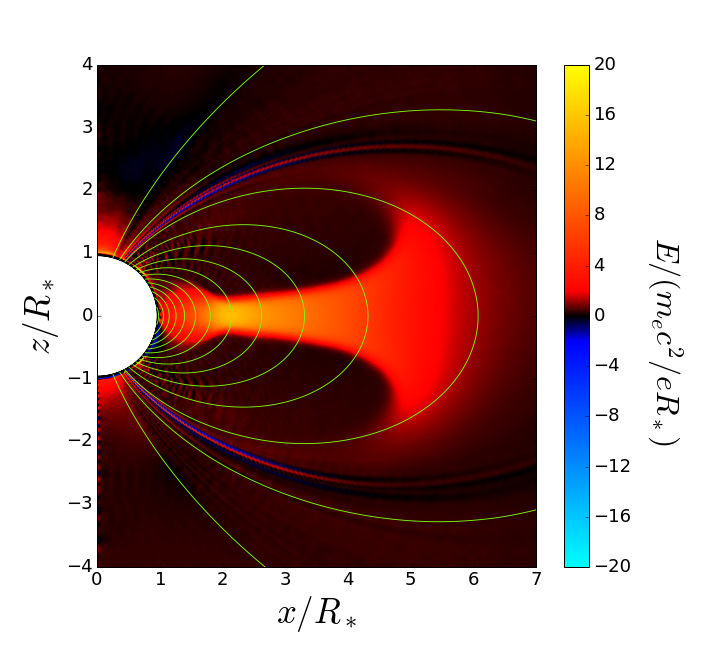
\includegraphics[width=0.7\textwidth]{pics/chap4/EdotB.png}
  \caption[Electric gap in magnetar magnetosphere]{Electric gap in the twisted
    magnetosphere. Magnetic field lines are shown by the green curves (poloidal
    cross section), and color shows the parallel electric field, defined as
    $E_\parallel=\mathbf{E}\cdot \mathbf{B}/B$, in our standard units defined in
    Section~\ref{sec:units}. The plot shows the average of a series of snapshots
    centered around $\tilde{t} = 200$. The gap voltage is self-regulated to the
    discharge threshold $\gthr$; $\gthr=10$ in the simulation.}
  \label{fig:EdotB}
\end{figure}
%%%%%%%%%%%%%%%%%%%%%%%%%%%%%%%

As seen in Figure~\ref{fig:EdotB}, the gap has a rather sharp boundary;
$E_\parallel$ is screened outside it by the created $e^\pm$ plasma.
The drop of $E_\parallel$ across the two boundaries of the gap is sustained by the layers
of positive and negative charge ($\pm\Sigma$ above and below the equatorial plane,
respectively), according to Gauss law $\nabla\cdot\bE=4\pi\rho$.
The charged layers are self-consistently sustained by the difference in velocities of
positive and negative charges passing through them in the self-organized $E_\parallel$.

In essence, the gap is a double layer. It has been compressed toward
the equatorial plane to a minimum thickness $\lgap$ that is still capable of sustaining
particle acceleration to $\gthr$.
Similar to the double layer described in Section~\ref{sec:v-no-pair}, the charge layers sandwiching
the gap have the thickness comparable to the local plasma skin depth $\lambda_p$
(evaluated for charge density $\sim j/c$) (Figure \ref{fig:rho}).
The electric field in the gap is $\Egap\sim 4\pi (j/c)\lambda_p$ and its voltage is
\begin{equation}
  e\Phigap\sim \frac{\lgap}{\lambda_p}\,m_ec^2.
\end{equation}
The self-regulation of the gap voltage to $\Phigap\approx \Phi_{\rm thr}$
controls the gap thickness $\lgap\sim\gthr\lambda_p$.

%%%%%%%%%%%%%%%%%%%%%%%%%%%%
\begin{figure}[t]
  \centering
  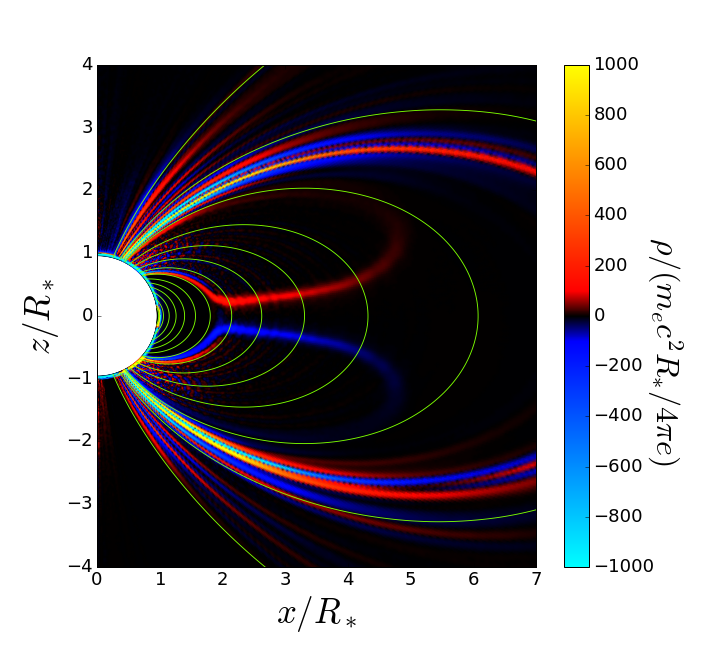
\includegraphics[width=0.7\textwidth]{pics/chap4/Rho.png}
  \caption[Charge density in magnetar magnetosphere]{Charge density in the magnetosphere, averaged in the
    same way as in Figure \ref{fig:EdotB}. Note the thin charged layers bounding
    the equatorial gap across the magnetic field lines. The layers extend into
    the inner magnetosphere along the inner boundary of the j-bundle. The
    charged structure observed on the field lines extending to $\tilde{r}\sim 9$
    approximately corresponds to the outer boundary of the j-bundle (see
    Figure~\ref{fig:current}).}
  \label{fig:rho}
\end{figure}
%%%%%%%%%%%%%%%%%%%%%%%%%%%%

Unlike normal double layers, particles accelerated in the gap are not brought
from outside; instead, the gap feeds itself with particles. The accelerated
particles create secondary $e^\pm$ of lower energies near the gap exit, and some
of the secondary particles are reversed by $E_\parallel$ and accelerated toward
the opposite boundary of the gap, where they create new pairs, etc.


%%%%%%%%%%%%%%%%%%%%%%%%%%%%%%%
\begin{figure}[t]
  \centering
  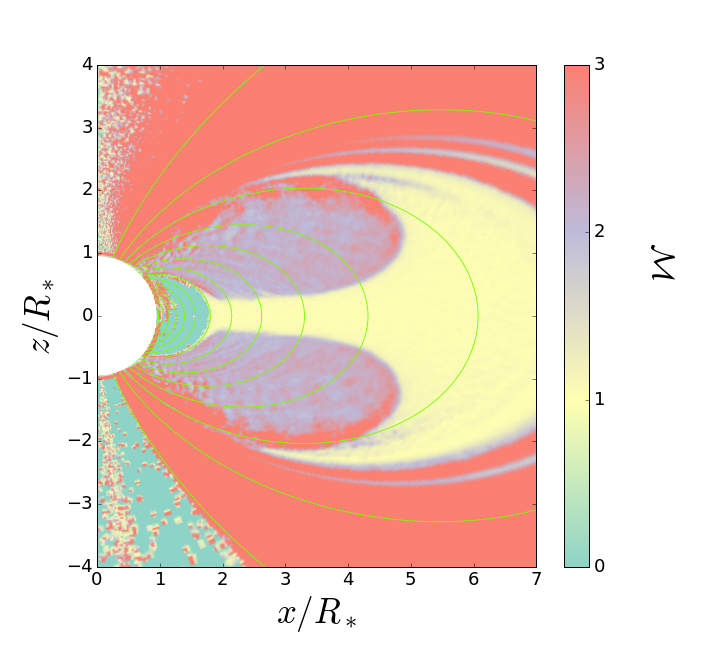
\includegraphics[width=0.7\textwidth]{pics/chap4/multiplicity.png}
  \caption[Magnetar magnetospheric pair multiplicity]{Pair multiplicity
    $\mathcal{M} = (\rho_+ - \rho_{-})c/j$.}
  \label{fig:multiplicity}
\end{figure}
%%%%%%%%%%%%%%%%%%%%%%%%%%%%%%%

The multiplicity of the pair plasma is defined by $\mathcal{M} = (\rho_+-\rho_{-})c/j$,
where $\rho_+$ and $\rho_-$ are the charge densities of the positrons and electrons,
respectively. One can see in Figure~\ref{fig:multiplicity} that $\mathcal{M}$
in the gap is close to 1, i.e. the gap contains the minimum amount of plasma needed to
conduct the electric current.
This is consistent
with no screening in the gap that allows the strong $E_\parallel$ to be
sustained. Pair multiplicity in other parts of the j-bundle is
close to 2,
just sufficient to screen $E_\parallel$. Apparently, the discharge in the
simulation is self-organized to carry the current with the minimum voltage
$\Phi_e\approx\Phigap\approx\Phi_{\rm thr}$ and the minimum rate of pair
creation.

Figure~\ref{fig:momenta} shows the average hydrodynamic momenta of
electrons and positrons. It is apparent that both species are accelerated across the
equatorial gap to the threshold Lorentz factor $\gthr=10$. The move with almost
speed of light in the opposite directions and make approximately equal contributions
to the current density, consistent with $\M\approx 1$.
Outside the gap,
$\M\approx 2$ together with the charge neutrality condition $n_+\approx n_-$
implies that the current is carried by one species while the other creates the
neutralizing, nearly static, background. This is indeed observed in
Figure~\ref{fig:momenta}.

The gap voltage is not exactly steady and shows quasi-periodic ``breathing'' with time.
This must assist the gap in reversing some of the secondary particles so that
they can cross the gap and accelerate to $\gthr$, sustaining the pair creation cycle.
Most of the accelerated particles escape the gap and get absorbed by the star.

%%%%%%%%%%%%%%%%%%%%%%%%%%%%%
\begin{figure*}[t]
  \centering
  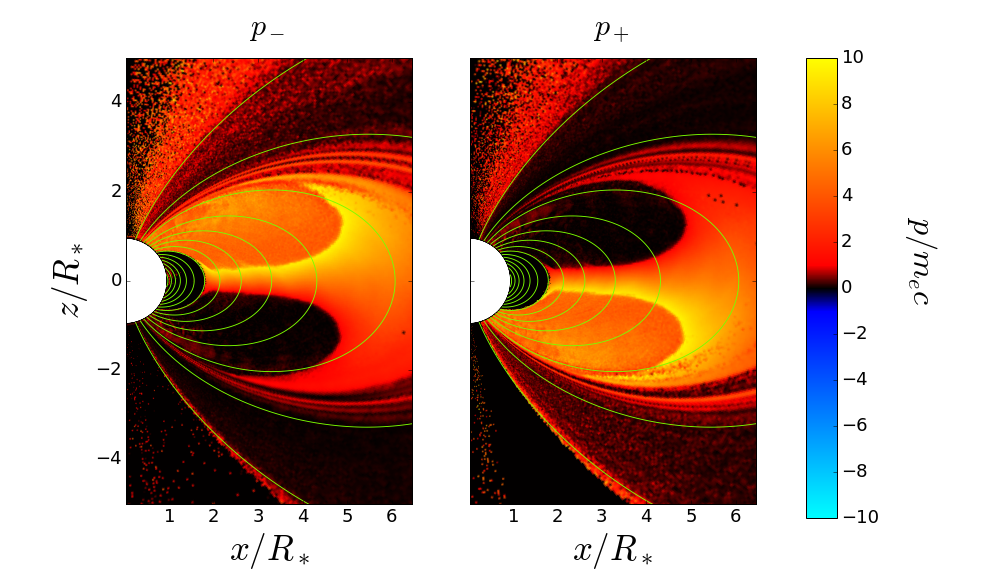
\includegraphics[width=0.9\textwidth]{pics/chap4/momentum.png}
  \caption[Average hydrodynamic momenta in magnetar magnetosphere]{Average hydrodynamic momentum of electrons (left) and positrons (right).}
  \label{fig:momenta}
\end{figure*}
%%%%%%%%%%%%%%%%%%%%%%%%%%%%%


Since the magnetosphere was set up to be symmetric about the equatorial plane,
the fact that the current is strongly dominated by created pairs  implies
symmetric bombardment of the two footprints of the j-bundle. Thus, our simulation
shows two symmetric hot spots (or rather rings, due to the axial symmetry) in the
northern and southern hemispheres of the star.

As discussed in BT07 and Section~\ref{sec:v-no-pair}, the voltage $\Phi_e$ in
the magnetospheric circuit is purely inductive. The parallel electric field
$\bE= -c^{-1}\partial \mathbf{A}/\partial t$ is associated with the slow
dissipation of $B_{\phi}$ rather than an electrostatic potential.
Note also that the dissipation rate $\bE\cdot\bj=E_\parallel j$ is localized in the
gap while the untwisting of $B_\phi$ also occurs outside the gap. The re-distribution of the
dissipated $B_\phi$ along the j-bundle into the screened region with $E_\parallel\approx 0$
occurs through the Alfv\'en mode, which can propagate without dissipation.
The Alfv\'en timescale $\tA\sim r/c$ is much shorter than the untwisting timescale $\tev$,
and so the magnetosphere slowly evolves through the sequence of global twist equilibria
of a decreasing energy
$\Etw$,
even though the magnetic energy is converted to heat only
near the equator.


\subsection{Dependence on the threshold voltage}
\label{sec:voltage}


While the simulation with $\gthr=10$ is the most adequate re-scaled version of the
magnetar magnetosphere (Section~\ref{sec:rescale}), we also performed simulations with
$\gthr=20$, 100, and $\infty$ (no pair creation). All other parameters of the four
simulations were identical.

Figure \ref{fig:b-energy} shows the evolution of the twist energy $\Etw$
in the simulations with the four different values of $\gthr$. An obvious trend is observed:
a higher threshold voltage for discharge, $e\Phithr=\gthr m_ec^2$, leads to a higher
dissipation rate and a shorter lifetime of the magnetic twist. When $\gthr\gg 10$,
the dissipation becomes so strong that it affects the initial stage of the twist
implantation at $\tilde{t}<\tilde{t}_\mathrm{shear}=40$, so that a substantial part of the twist amplitude
(and the corresponding energy $\Etw$) is lost before it could be implanted.

The extreme model with $\gthr=\infty$ gives so strong dissipation that $\Etw$
does not reach even 10\% of its target value. It is instructive to compare this
simulation with the expected dissipation rate in the pair-free configuration
described in Section~\ref{sec:v-no-pair}. From equation \eqref{eq:voltage}, we
can estimate the voltage drop of the double layer as $\gDL=\tilde{\Phi}_{e} \sim
\sqrt{\tilde{\jmath}}\,\tilde{W}$. The initial width of the j-bundle near the
star is $\tilde{W}\sim 1$. The target current density reaches $\tilde{\jmath}
\sim 3\times 10^4$ if the twist is fully implanted. This estimate gives $\gDL$
comparable to $200$; the actual voltage in the simulation reaches somewhat
higher values. The high voltage develops early during the shearing stage and
results in strong dissipation, which does not allow $\tilde{j}$ to approach
$3\times 10^4$.

The simulation with $\gthr=100$ enables the pair discharge, which buffers the
voltage growth in the j-bundle and allows a stronger twist to be implanted.
The simulations with $\gamma_\mathrm{thr}=20$ and, in particular, $\gthr=10$,
allow almost full implantation of the target twist with small ohmic losses. The subsequent  slow resistive evolution is similar in the two models, as both have $\Phithr$ well below
the double-layer voltage and sustain a long-lived discharge activity in the j-bundle.
As expected, the untwisting timescale $\tev$ is reduced by a factor of $2$ as
$\gthr$ is increased from 10 to 20 (see \Eq~\ref{eq:tev}).


%%%%%%%%%%%%%%%%%%%%%%%%%%%%%%%%%
\begin{figure}[t]
  \centering
  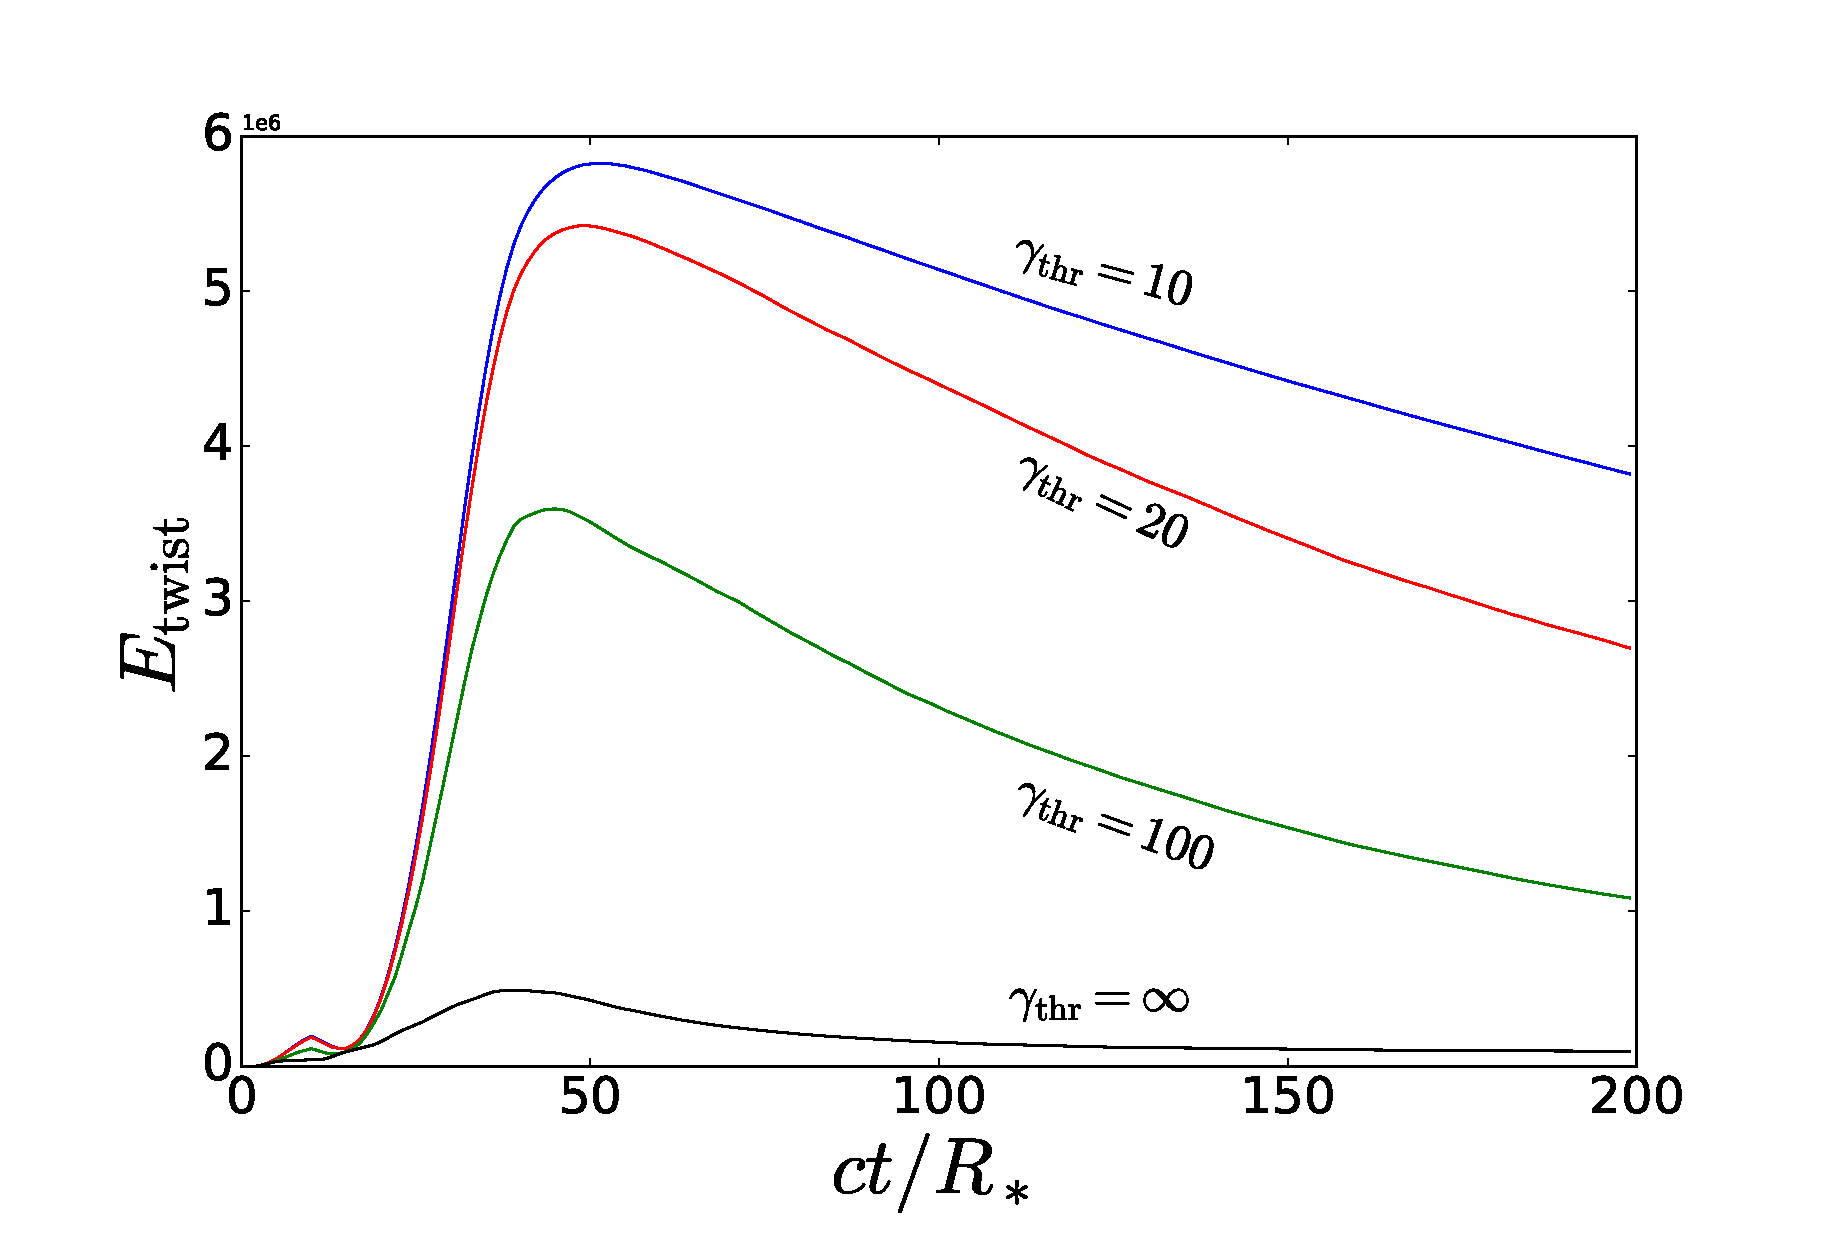
\includegraphics[width=0.8\textwidth]{pics/chap4/B-energy.eps}
  \caption[Evolution of energy in the magnetar magnetosphere]{Evolution of the
    twist magnetic energy $\Etw$. Four simulations are shown with discharge
    thresholds $\gthr=10$, 20, 100, $\infty$. We use the exact expression for
    $\Etw = \int (B^2 - B_0^2)/8\pi\, dV$, where $B_0$ is the initial dipole
    field. It takes into account that besides $B_\phi^2/8\pi$ part of the twist
    energy is stored in the inflated poloidal magnetic field, which becomes
    important when the twist amplitude $\psi$ exceeds unity. }
  \label{fig:b-energy}
\end{figure}
%%%%%%%%%%%%%%%%%%%%%%%%%%%%%%%%%

These results unambiguously demonstrate that the energy dissipation timescale is
controlled by the pair creation threshold, confirming the conclusion of BT07.
In real magnetars, we expect $\gthr\ll\gDL$ (Section~\ref{sec:theory}).
Therefore, the most relevant model is the one with low $\gthr=10$, which is still high
enough to accelerated particles to ultra-relativistic energies and produce relativistic
secondary $e^\pm$.

\subsection{Expanding cavity}
\label{sec:untwisting}

Figure~\ref{fig:current} shows the resistive evolution of the j-bundle.
The untwisting of the magnetic field lines proceeds as anticipated
in
Section~\ref{sec:twist-theory}, through formation of a cavity $j=0$ that expands
from the inner magnetosphere near the equator (large flux function $u$).
Figure \ref{fig:jp} shows the evolution of the poloidal current $j_p$ until
the end of the simulation at $\tilde{t}_\mathrm{sim}=350$.
We chose to show $j_p/B_p$ because this quantity is constant along the magnetic
field lines (after averaging over short-timescale fluctuations), as expected in
a nearly force-free magnetosphere --- currents flow along the magnetic field lines.
Therefore, $j_p/B_p$ is a function of the magnetic field line, which we label
by the parameter $u=\sin^2\theta_\star$ (see \Eq~\ref{eq:u}).
Note the expansion of the region where $j_p = 0$ toward the magnetic axis,
from $u\approx 0.75$ to $u\lesssim 0.55$.

%%%%%%%%%%%%%%%%%%%%%%%%%%%%%%%
\begin{figure*}[t]
  \centering
  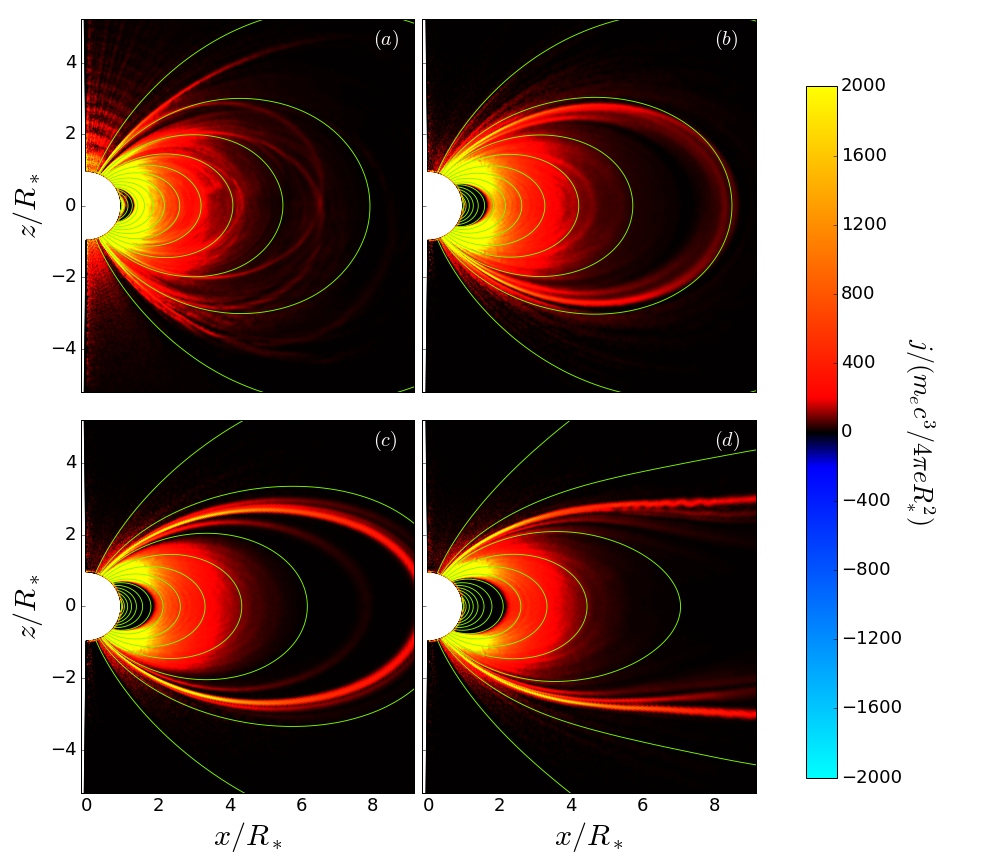
\includegraphics[width=0.9\textwidth]{pics/chap4/j-p-color.png}
  \caption[Evolution of the poloidal current density in magnetar
  magnetosphere]{Color plot showing the evolution of the poloidal current
    density $j_p$ in the simulation with $\gthr=10$. Four snapshots are shown:
    (a) $\tilde{t}=30$, (b) $\tilde{t}=120$, (b) $\tilde{t}=230$, and (d)
    $\tilde{t}=350$. Note that when $j_p=0$ then also $j=0$.}
  \label{fig:current}
\end{figure*}
%%%%%%%%%%%%%%%%%%%%%%%%%%%%%%%


%%%%%%%%%%%%%%%%%%%%%%%%%%%%%%%%%%
\begin{figure}[t]
  \centering
  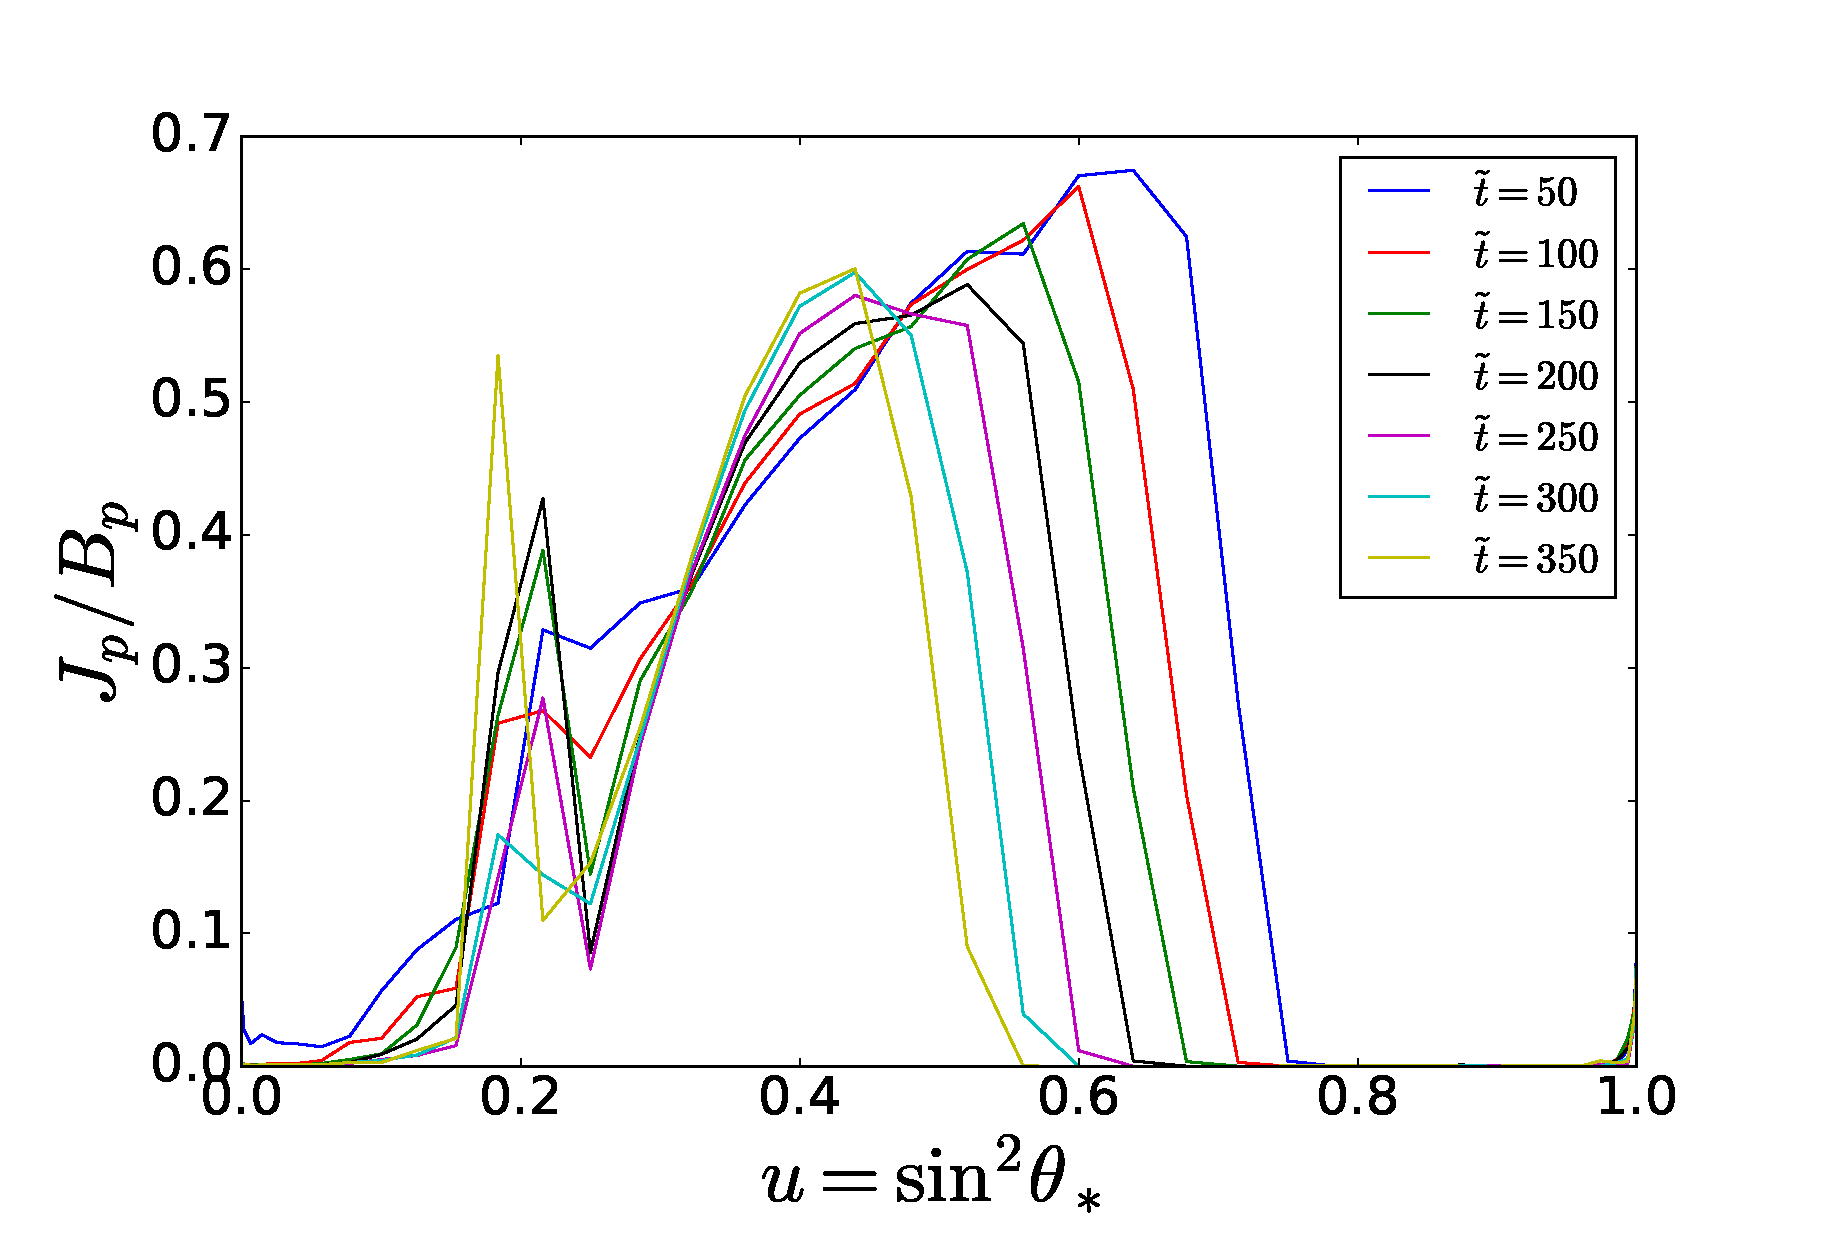
\includegraphics[width=0.75\textwidth]{pics/chap4/j-p.eps}
  \caption[Time evolution of the integrated current in magnetar
  magnetosphere]{Evolution of the poloidal current distribution in the
    magnetosphere in the simulation with $\gthr=10$. The ratio $j_p/B_p$
    (constant along the magnetic field lines) is shown versus the poloidal flux
    function defined in \Eq~(\ref{eq:u}); $\theta_\star$ is the polar angle of
    magnetic field line footprint on the star. The different curves show
    snapshots at times $\tilde{t}=50$, 100, 150, 200, 250, 300, and 350.}
  \label{fig:jp}
\end{figure}
%%%%%%%%%%%%%%%%%%%%%%%%%%%%%%%%%%

Figure \ref{fig:twist} shows the evolution of the integrated twist angle $\psi$
defined in Equation~\eqref{eq:twist-angle}. The untwisting proceeds from near
the equator, where the twist angle decreases over time, but the twist angle is
not simply erased, but relocated from the inner magnetosphere to the outer
parts, as expected from the untwisting Equation~\eqref{eq:twist-ev}.

%%%%%%%%%%%%%%%%%%%%%%%%%%%%%%%%%%
\begin{figure}[t]
  \centering
  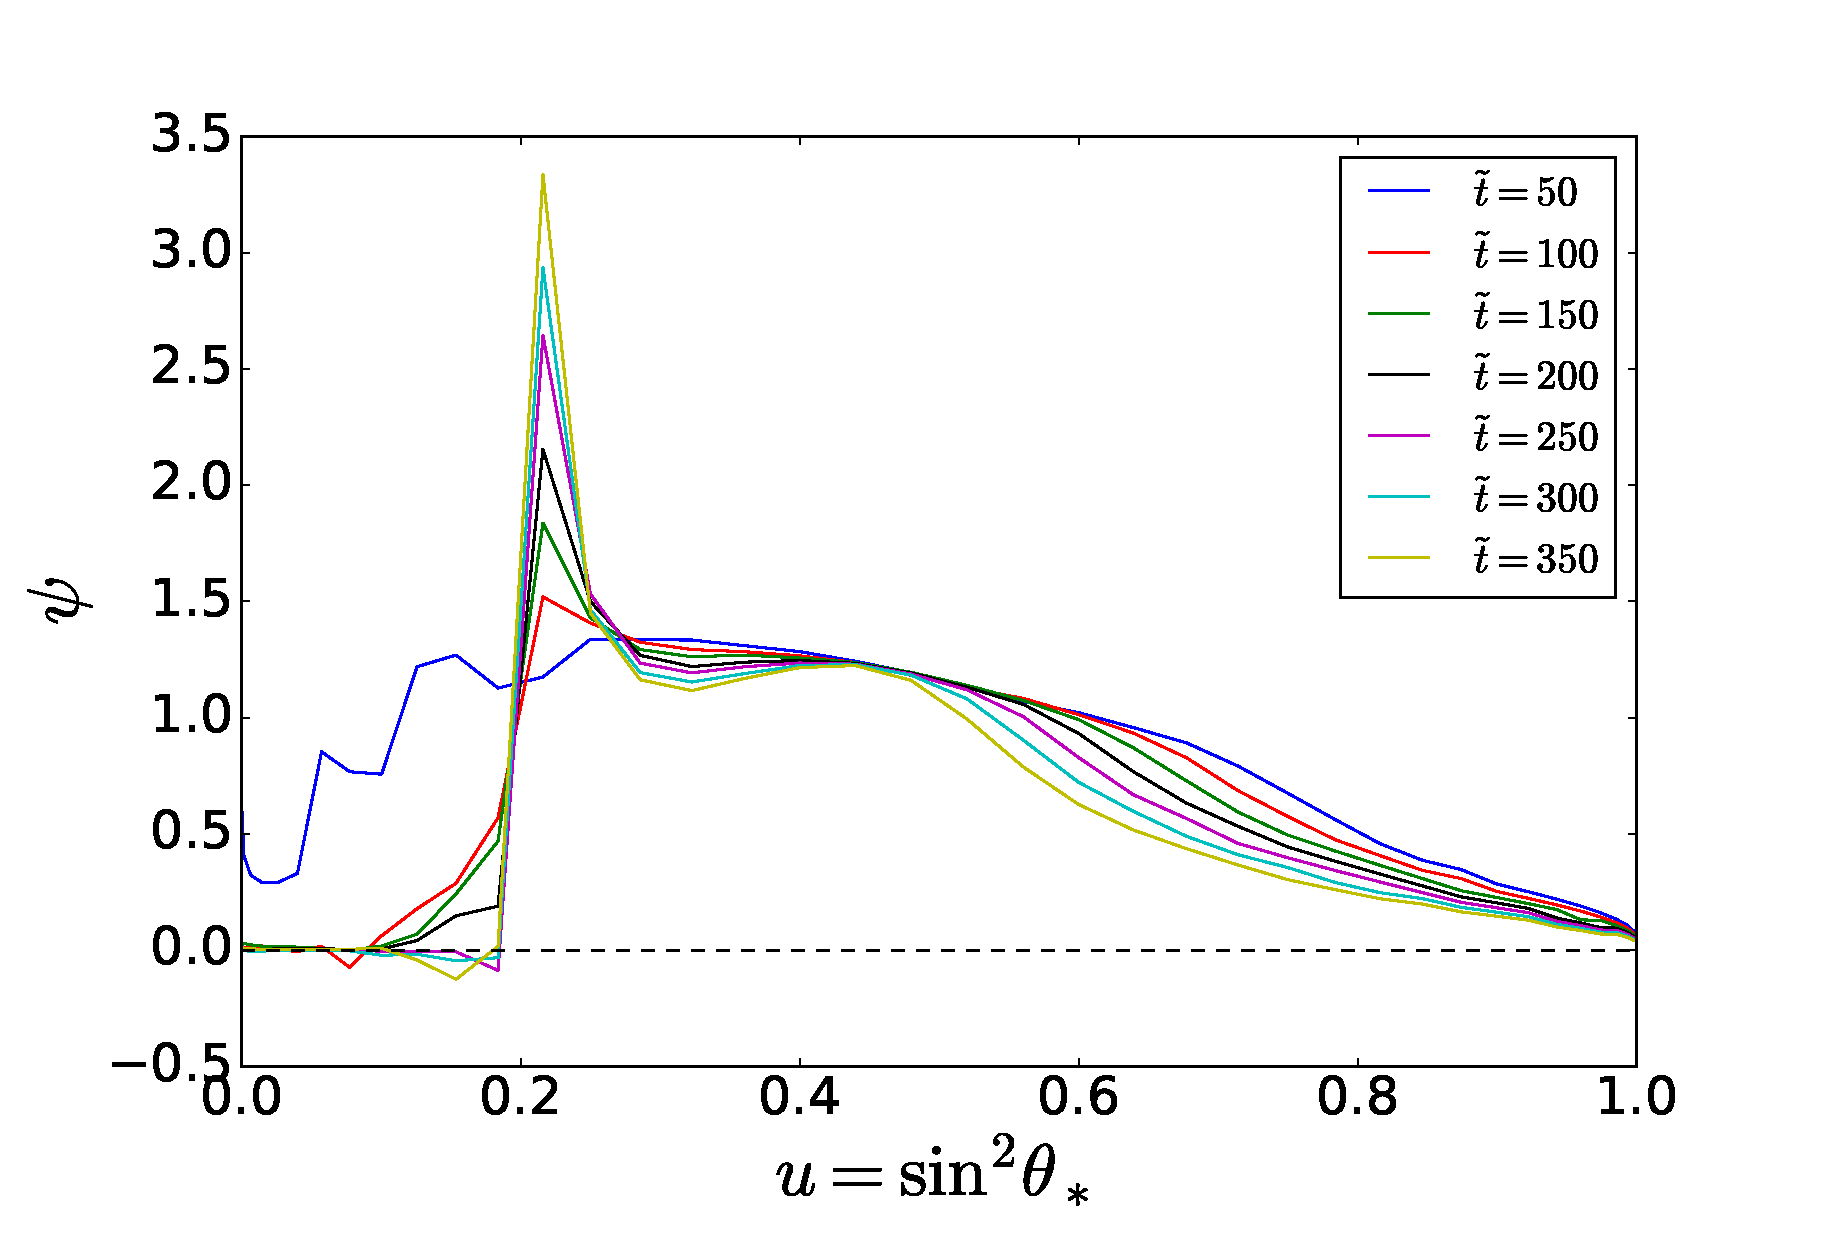
\includegraphics[width=0.75\textwidth]{pics/chap4/twist-evolution.eps}
  \caption[Evolution of the magnetar magnetospheric twist angle]{Evolution of
    the twist angle $\psi$ in the simulation with $\gamma_\mathrm{thr} = 10$. }
  \label{fig:twist}
\end{figure}
%%%%%%%%%%%%%%%%%%%%%%%%%%%%%%%%%%

A curious feature is observed to develop on the magnetic field lines with $u$
around 0.22: the twist angle $\psi$ {\it grows} and approaches 3.5 toward the end
of the simulation. This feature is also seen in the current structure shown
in Figures~\ref{fig:current} and \ref{fig:jp}. The strongly twisted, narrow bundle
of field lines is inflating with time and eventually opens up, causing a
magnetospheric instability (cf. PBH13).
Our simulation stopped right
 at the onset of this development, since we would like to limit our study to the
 quasi-steady untwisting regime.
An important difference from over-twisting studied in PBH13
is that here it is not driven by excessive surface shear. Instead, it results from
resistive evolution of the implanted twist while the crust is static.



\section{Discussion}
\label{sec:discussion}


We have performed the first axisymmetric particle-in-cell simulations of the
twisted magnetospheres of magnetars. The simulations demonstrate from
first principles that electric $e^\pm$ discharge is self-organized in the magnetosphere
to sustain the electric current $j$ demanded by the magnetospheric twist.

The results of our numerical experiment may be summarized as follows.
\begin{enumerate}
\item Shear motion of the stellar surface on a timescale $\ttw<\tev$
successfully implants a magnetic twist in the magnetosphere.
The twist is supported by continual electric current due to
self-organized $e^\pm$ discharge.

\item Particles are accelerated along the magnetic field lines to Lorentz factors
$\gamma\approx\gthr$, just sufficient to ignite pair creation.
The voltage sustaining the electric circuit, the
dissipation rate, and the lifetime of the twist are all regulated by $\gthr$.

\item Particle acceleration is localized in a gap near the equatorial plane
(Figure~\ref{fig:EdotB}).
The gap has the electric field $E_\parallel\sim 4\pi (j/c)\lambda_p$ and width
$\lgap\sim\gthr\lambda_p$, where $\lambda_p=(m_ec^3/4\pi e j)^{1/2}$ is the local
plasma skin-depth.
The plasma density in the gap is close to the minimum value $n=j/ec$ required to
conduct the electric current. Continual $e^\pm$ creation occurs near the two exits
from the gap.

\item The magnetospheric current is carried by electrons and positrons created
in the magnetosphere rather than electrons and ions extracted from the atmospheric
layer on the stellar surface. The created particles rain onto the footprints of the j-bundle,
creating two hot spots.

\item Resistive untwisting of the magnetosphere occurs on the timescale
$\tev$
estimated in \Eq~(\ref{eq:tev}), in agreement with theoretical expectations.
The evolution proceeds as predicted in B09: a cavity with $j=0$ quickly forms in
the inner magnetosphere and gradually expands, erasing the remaining electric currents.

\item A curious feature was observed in the untwisting process: while the
twist energy was decreasing as expected from ohmic dissipation,
the twist amplitude $\psi$ {\it grew} in a narrow bundle of field lines at the outer
boundary of the twisted region. This over-twisted bundle inflated so much that it
eventually opened up.
\end{enumerate}

Our results confirm that the untwisting magnetospheres naturally create shrinking hot
spots (footprints of the shrinking $j$-bundle), which have been detected in 7 transient
magnetars. The evolution timescale inferred from the simulations (\Eq~\ref{eq:tev})
is consistent with the decay timescale observed in transient magnetars (months to years).

One unknown in the setup of our numerical experiment is the profile of the
surface shear. However, basic features observed in the simulation, in particular
voltage regulation through $e^\pm$ discharge and the cavity expansion, should be
generic and independent of the details of the twist profile. It is less clear
how generic is the formation of the narrow over-twisted bundle. This could be
further explored with simulations of different shear profiles.

An important caveat in the simulation setup is the simplified ``on the spot''
prescription for pair creation, with the created $e^\pm$ pair taking a
significant energy fraction from the primary particle. As briefly discussed in
Section~\ref{sec:pairs}, this prescription is reasonable if the twist is
confined to the region of ultrastrong magnetic field near the star, $B\gtrsim
B_Q$. Pair creation in weaker fields tends to occur with high multiplicities,
which can launch a dense $e^\pm$ outflow and efficiently screen $E_\parallel$ in
the equatorial region \citep{beloborodov_mechanism_2013}. Then the gap may have to
split into two gaps and move away from the equator, closer to the star.

How the discharge will self-organize in this case can only be explored using a
more detailed implementation of the pair creation process. The future simulation
will directly track the high-energy photons produced by resonant
scattering and their conversion to pairs, without prescribing any $\gthr$.
This will be the focus of our future work, and we expect it to establish the gap location
on magnetic field lines extending far from the star. This part of the magnetosphere is
interesting for two reasons: (1) the j-bundle activity tends to
concentrate on the extended field lines, and (2) the nonthermal emission
is able to escape the outer magnetosphere while almost all resonantly scattered
photons in the region $B\gg10^{13}$~G convert to pairs \citep{beloborodov_mechanism_2013}.
Gap location on the extended field lines influences the hard X-ray spectrum
emitted by the twisted magnetosphere, and thus can be tested against observations.
Phase-resolved hard X-ray spectra have been measured for several magnetars
and fitted by the $e^\pm$ outflow model
% (e.g. Hasco\"et et al. 2014; An et al. 2015),
\citetext{e.g. \citealp{hascoet_phase-resolved_2014}; \citealp{an_deep_2015}},
which assumes an electric gap near the star. Direct PIC simulations of the $e^\pm$
discharge
of high
multiplicity can verify or disprove this assumption.


We did not study in this chapter what happens when the magnetosphere is
over-twisted and becomes unstable. This phenomenon is associated with the
observed giant flares of magnetars, an extreme analogy of solar flares. The
over-twisted magnetosphere inflates and creates a thin current sheet separating
magnetic fluxes of opposite polarities. The current sheet becomes
unstable to the tearing mode, which leads to magnetic reconnection and ejection
of plasmoids from the magnetosphere (\citealp{lyutikov_explosive_2003}; PBH13), resembling the
mechanism of coronal mass ejections from the sun
% (e.g. Mikic \& Linker 1994).
\cite[e.g.][]{mikic_disruption_1994}.
Our preliminary studies using Aperture show similar behavior.
One difficulty encountered by such simulations is the huge pair creation rate
in the dissipative current sheet, which must result in quick thermalization
of the released magnetic energy. A scheme describing this transition needs to
be developed and will be a topic for future work.

% Local Variables:
% TeX-master: "../thesis"
% zotero-collection: #("16" 0 2 (name "Thesis"))
% End:

%%%%%%%%%%%%%%%%%%%%%%%%%%%% Reference %%%%%%%%%%%%%%%%%%%%%%%%%%%%%%
\bibliographystyle{apj}
\pagestyle{myheadings}
\markright{}
\bibliography{thesis}

%%%%%%%%%%%%%%%%%%%%%%%%%%%% Appendix %%%%%%%%%%%%%%%%%%%%%%%%%%%%%%
\begin{appendices}
% \input{appendix/PhysicalParameters.tex}
\end{appendices}

\end{document}


%%% Local Variables:
%%% zotero-collection: #("16" 0 2 (name "Thesis"))
%%% mode: latex
%%% TeX-engine: luatex
%%% End:
